\documentclass[a4paper, 12pt, oneside]{report} % for final draft compilation
% \documentclass[a4paper, 12pt, oneside, draft]{report} % for draft compilation

% Preamble:
\usepackage[T1]{fontenc}                                 % package for specifying output font encoding
\usepackage[acronym,style=super,nogroupskip]{glossaries} % package for making glossaries
\usepackage[flushleft]{threeparttablex}                  % package to add notes at the bottom of the table
\usepackage[font=footnotesize,format=hang]{caption}      % package for formatting figure caption
\usepackage[hidelinks, colorlinks]{hyperref}             % package for hyperlinking references - hidelinks option removes the ugly boxes around the huperlinks
\usepackage[md]{titlesec}                                % package for tweaking the chapter/section/subsection titles format
\usepackage[noabbrev,capitalise]{cleveref}               % package for referencing multiple referencing in a single \ref command
\usepackage[toc]{appendix}                               % package for making appendices
\usepackage[utf8]{inputenc}                              % package for specifying input font encoding
\usepackage{chngcntr}                                    % package for making continuous figure numbering, instead of section-based numbering
\usepackage{graphicx}                                    % package for graphics handling (i.e. figure images)
\usepackage{mathptmx}                                    % package for Times New Roman font
\usepackage{natbib}                                      % package for reference management
\usepackage{setspace}                                    % package for setting line space (used in title page)
\usepackage{xcolor,colortbl}                             % package for making colours
\usepackage{booktabs}                                    % package for better looking tables
\usepackage{longtable}                                   % package for tables that span multiple pages
\usepackage{siunitx}                                     % package for scientific notations and units
\usepackage{etoolbox}                                    % package to 'robustify' \bfseries

% Define colour(s) for table rows:
\definecolor{LightCyan}{rgb}{0.88,1,1}

% Set up the hyperlinks - change the colour of the links to blue:
% \hypersetup{allcolors=blue}
\hypersetup{allcolors=black} % uncomment this line to make the hyperlinks black

% Change the default cref name for equations:
\creflabelformat{equation}{#2\textup{#1}#3}

% Change the default cref name for appendix:
\crefname{appcha}{Appendix}{Appendices}
\crefname{appsec}{Appendix}{Appendices}

% Make siunitx detect bold/italics/etc:
\robustify\bfseries
\sisetup{detect-all}

% Set the width of captions for threeparttable to \linewidth:
\captionsetup[threeparttable]{width=\linewidth}

% Set up continuous figures:
\DeclareCaptionFormat{cont}{#1 (cont.)\par}

% Change the default url font:
\urlstyle{rm}

% change figure numbering from section-based to continuous:
\counterwithout{figure}{chapter}
\counterwithout{equation}{chapter}
\counterwithout{table}{chapter}

% Change the title of bibliography to references:
\renewcommand{\bibname}{References}

% Change the title of Table of Contents:
\renewcommand{\contentsname}{Table of Contents}

% Change the title of Table of Contents:
% \renewcommand{\thesubfigure}{\Alph{subfigure}}

% Italicise the subsubsection title:
\titleformat{\subsubsection}{\normalfont\itshape\bfseries}{\thesubsubsection}{1em}{}
\titleformat{\paragraph}{\normalfont\itshape}{\theparagraph}{\noindent}{}

% Remove unnecessary spaces between the figures from different chapters in LoF and LoT:
\newcommand*{\noaddvspace}{\renewcommand*{\addvspace}[1]{}}
\addtocontents{lof}{\protect\noaddvspace}
\addtocontents{lot}{\protect\noaddvspace}

% For generating glossaries:
%%%%%%%%%%%%%%%%%%%%%%%%%%%%%%%%%%%%%%%%%%%%%%%%%%%%%%%%%%%%%%%%%%%%%%%%%%%%%%%
%% Glossary terms
%%%%%%%%%%%%%%%%%%%%%%%%%%%%%%%%%%%%%%%%%%%%%%%%%%%%%%%%%%%%%%%%%%%%%%%%%%%%%%%

% TODO: make sure you get a proper definitions for all of these glossary terms

\newglossaryentry{rnaseq}{
	name=RNA-seq,
	description={sequence data using transcriptome}
}

\newglossaryentry{r}{
	name=R,
	description={Statistical programming language}
}

\newglossaryentry{metagene}{
	name=Metagene,
	text=metagene,
	description={Summary score of a sample that represents the overall gene expression of the genes that was used to obtain the scores}
}

%%%%%%%%%%%%%%%%%%%%%%%%%%%%%%%%%%%%%%%%%%%%%%%%%%%%%%%%%%%%%%%%%%%%%%%%%%%%%%%
%% Acronym terms
%%%%%%%%%%%%%%%%%%%%%%%%%%%%%%%%%%%%%%%%%%%%%%%%%%%%%%%%%%%%%%%%%%%%%%%%%%%%%%%

\newacronym{blca}{BLCA}{bladder urothelial carcinoma}
\newacronym{cesc}{CESC}{cervical squamous cell carcinoma and endocervical adenocarcinoma}
\newacronym{coad}{COAD}{colon adenocarcinoma}
\newacronym{kirp}{KIRP}{kidney renal clear cell carcinoma}
\newacronym{lihc}{LIHC}{liver hepatocellular carcinoma}
\newacronym{read}{READ}{rectum adenocarcinoma}
\newacronym{skcm}{SKCM}{skin cutaneous melanoma}
\newacronym{ucec}{UCEC}{uterine corpus endometrial carcinoma}
\newacronym{geo}{GEO}{Gene Expression Omnibus}
\newacronym{tcga}{TCGA}{The Cancer Genome Atlas}
\newacronym{icgc}{ICGC}{International Cancer Genome Consortium}
\newacronym{bmi}{BMI}{Body Mass Index}
\newacronym{who}{WHO}{World Health Organization}
\newacronym{ln}{LN}{Lymph node}
\newacronym{pr}{PR}{Progesterone receptor}
\newacronym{er}{ER}{Estrogen receptor}
\newacronym{her2}{HER2}{Human epidermal growth factor receptor 2}
\newacronym{svd}{SVD}{Singular value decomposition}
\newacronym{rma}{RMA}{Robust Multi Array}
\newacronym{mas}{MAS5}{Microarray Analysis Suite 5.0}
\newacronym{fdr}{FDR}{False Discovery Rate}
\newacronym{go}{GO}{Gene Ontology}
\newacronym[longplural={Disability-Adjusted Life Years}]{daly}{DALY}{Disability-Adjusted Life Year}


\makeglossaries

% Specify graphics path:
\graphicspath{{./images/}}
\DeclareGraphicsExtensions{.pdf,.png,.jpg}

% If you want to compile specific files, uncomment the line below and add the filenames in the {} :
% \includeonly{{./misc/title},{./misc/abstract},{./misc/acknowledgement},{./methods/methods},{./intro/intro},{./results/results},{./results/results2},{./discussion/discussion}}
% \includeonly{{./misc/title},{./misc/abstract},{./misc/acknowledgement}}
% \includeonly{{./intro/intro}}
% \includeonly{{./methods/methods}}
% \includeonly{{./results/results2},{./discussion/discussion},{./misc/appendix},{./misc/appendix2}}
% \includeonly{{./results/results}}
% \includeonly{{./results/results2}}
% \includeonly{{./discussion/discussion}}
% \includeonly{{./misc/appendix}}
% \includeonly{{./misc/appendix2}}

% Define some alias for very long citations:
\defcitealias{TCGA}{NCI and NHGRI, 2016}
\defcitealias{ICGC}{ICGC, 2016}
\defcitealias{GEO}{NCBI, 2016}

\begin{document}

% Set line spacing to double space:
\onehalfspacing

%%%%%%%%%%%%%%%%%%%%%%%%%%%%%%%%%%%%%%%%%%%%%%%%%%%%%%%%%%%%
% Title page for my thesis - code is pretty self explanatory
% Required packages: setspace
%%%%%%%%%%%%%%%%%%%%%%%%%%%%%%%%%%%%%%%%%%%%%%%%%%%%%%%%%%%%
\begin{titlepage}

\centering

\rule[2.0mm]{\textwidth}{0.5mm}

\begin{doublespace}
    {\Huge \scshape Body Mass Index and Pathway Dysregulation in Cancer}
\end{doublespace}

\rule[2.0mm]{\textwidth}{0.5mm}

\vspace{2.0mm}
{\Large \scshape Riku Takei}

\vfill


\includegraphics[width=0.33\linewidth]{/misc/otago}

\vfill

{\normalsize \scshape A Thesis Submitted For The Degree Of\\}
{\Large \scshape Master Of Science\\}
\vspace{2.0mm}
{\normalsize \scshape At The University Of Otago, Dunedin, New Zealand \\}

\vspace{10.0mm}
{\normalsize \today}

\end{titlepage}


\pagenumbering{roman} % set page numbering to roman numeral

%%%%%%%%%%%%%%%%%%%%%%%%%%%%%%%%%%%%%%%%%%%%%%%%%%%%%%%%%%%%
% Abstract for my thesis
%%%%%%%%%%%%%%%%%%%%%%%%%%%%%%%%%%%%%%%%%%%%%%%%%%%%%%%%%%%%
\vspace*{\fill}

\section*{\centering Abstract}
\addcontentsline{toc}{section}{Abstract}

Obesity has been a major global problem for more than a decade, associated with many noncommunicable diseases such as  cancer.
The number of obese people, both adults and children, has risen in every country of the world and the trend will likely to continue.
Cancers are caused by dysregulation of various molecular pathways that allow tumour cells to proliferate, survive and migrate.
One of the difficulties associated with the treatment of cancers is the identification of the underlying biological pathways that drive tumorigenesis.
This research aims to determine whether gene expression signatures exist  that are specific to obesity across multiple cancer types, and to investigate whether there are any common pathways being dysregulated in cancers based on these genetic signatures.
In this work no genetic signatures or differentially expressed genes were found between obese and non-obese patients that were common across multiple cancer types.
However, the Akt, \gls{egfr}, \gls{tgfb} and Src pathways may have a role in promoting the tumour progression in patients that are obese.
It is likely that there is some complex mechanism underlying the relationship between obesity and cancer.
A better understanding of the pathways being dysregulated in cancer cells in obese patients may lead to improved clinical decisions, and contribute towards personalised treatment in the future.

\vfill
\vfill


%%%%%%%%%%%%%%%%%%%%%%%%%%%%%%%%%%%%%%%%%%%%%%%%%%%%%%%%%%%%
% Acknowledgement for my thesis
%%%%%%%%%%%%%%%%%%%%%%%%%%%%%%%%%%%%%%%%%%%%%%%%%%%%%%%%%%%%

\section*{\centering Acknowledgement}
\addcontentsline{toc}{section}{Acknowledgement}

%\begin{center}

This page is for acknowledgement

%\end{center}


\addcontentsline{toc}{section}{\contentsname}

\tableofcontents

\clearpage

\addcontentsline{toc}{section}{\listfigurename}

\listoffigures

\clearpage

\addcontentsline{toc}{section}{\listtablename}

\listoftables

\clearpage

\addcontentsline{toc}{section}{Glossary}

\printglossary[style=super]

% Need to set line spacing to single space, otherwise it inserts a blank page for an unknown reason:
\singlespacing

\clearpage

\addcontentsline{toc}{section}{Acronyms}

\printglossary[type=\acronymtype,style=super]

\clearpage

% Reset the spacing to 1.5:
\onehalfspacing

\pagenumbering{arabic} % revert the page numbering to normal numbering
\glsresetall

\chapter{Introduction (draft)}
\label{ch:intro}

% TODO: also have a look at the masters talk write up from 2015

\section{Obesity}
\label{sec:obesity}

% General intro to obesity.
% Implications of obesity -- disease associated with it and/or cancer.
Obesity has been one of the major global problems for more than a decade, associated with many noncommunicable diseases such as diabetes, cardiovascular diseases and certain types of cancers \citep{WHO2014}.
In fact, the risk of comorbidities increases with the increase in \gls{bmi}, where the risk becomes severe as the \gls{bmi} level approaches the obese category \citep{WHO2000}.

The number of overweight and obese population, in both adults and children, have risen in every country of the world, and the trend continues as we speak.
Estimated to account for 3.4 million deaths per year and 93.6 million \glspl{daly} in 2010, obesity is a serious disease that continues to grow in our society \citep{Lim2012}.

\subsection{Definition of obesity}
\label{sub:definition_of_obesity}
% TODO: add WHO website to the reference for the definition of obesity (or find proper articles)

Obesity is defined as an abnormal or excessive fat accumulation that may impair health of that individual \citep{Garrow1988}.

One common and widely used approach to categorise individuals is by measuring the \gls{bmi} of the individual.
\gls{bmi} is a measurement based on the weight-to-height ratio of an individual that is used by clinicians and epidemiologists to classify adults into underweight, normal weight, overweight or obese categories.
The unit of \gls{bmi} is defined as the individual's weight in kilograms per square of the height in meters (kg/m$^2$).

\gls{who} (2014) have used \gls{bmi} measurements to define overweight and obesity in adults as an individual with \gls{bmi} $\geq$ 25 kg/m$^2$ and $\geq$ 30 kg/m$^2$, respectively.
For children under the age of 5, overweight and obesity were defined as weight-for-height greater than 2 standard deviation and 3 standard deviation above \gls{who} Child Growth Standards median, respectively.
For children aged between 5 to 19 years, overweight and obesity were defined as BMI-for-age greater than 1 standard deviation and 2 standard deviation above \gls{who} Growth Reference Standards median, respectively.

Although the use of \gls{bmi} as an accurate measure of body fat composition and/or representation of the individual's metabolic status remains controversial, many studies have used \gls{bmi} due to the ease of data collection compared to other measurements, such as [example] (citation needed).
Consequently, most of the publicly available clinical data have height and weight data from which one can calculate the patients' \gls{bmi}, and therefore able to collect the patients' obesity status more conveniently than, for example, [example].

possible papers:\citep{Gelber2008, Lee2008, Yusuf2005}

\subsection{Prevalence of obesity}
\label{sub:prevalence_of_obesity}

From the latest global status report on noncommunicable diseases by \citet{WHO2014}:
\begin{quote}
	\textit{
		In 2014, 39\% of adults aged 18 years and older (38\% of men and 40\% of women) were overweight.
		The worldwide prevalence of obesity nearly doubled between 1980 and 2014.
		In 2014, 11\% of men and 15\% of women worldwide were obese.
		Thus, more than half a billion adults worldwide are classed as obese.
	}
\end{quote}

\noindent
This equated to approximately 1 in every 14 people in the world classed as obese in 2014, and therefore, 1 in 14 people around the world were also at severe health risks associated with obesity.
It was also noted in the report that women were more likely to be obese than men, and that the prevalence of overweight and obesity increased as the income level of the countries increased \citep{WHO2014}.

In addition to this, the worldwide prevalence of childhood overweight and obesity has been increasing steadily since 2000 \citep{WHO2014}.
Furthermore, the prevalence of overweight in children under 5 years was estimated to reach from 6.3\% in 2013 to 11\% by 2025 if the current trend continued \citep{WHO2014}.
The current obesity status of the adult population is bad already, but the fact that more of the younger population who are overweight and obese poses a much greater risk for the health of the population (discussed in \cref{sub:impact_of_obesity}).

Until these terrible trends stop, and even after the trends stop, the world will need a plan to live along with this ongoing global epidemic of obesity and its associated diseases.

\subsection{Physiological mechanism of obesity}
\label{sub:physiological_mechanism_of_obesity}

Obesity is caused by continuous intake of food, whether they are controlled or not, without expending all of the energy gained.
The key to the problem is the control of food intake and energy expenditure, and how they are regulated in your body.

\subsubsection{Role of hypothalamus and arcuate nucleus in food intake control}
\label{ssub:role_of_hypothalamus_and_arcuate_nucleus_in_food_intake_control}

The central role of hypothalamus in the context of obesity is the control of satiety, and therefore food intake.
The hypothalamus receives both nueronal and hormonal inputs from the body and propagates the signal to the downstream neurons that ultimately affect the food intake of the individual \citep{Bell2005, Spiegelman2001}.

Within the hypothalamus, there is a group of neurons located within the arcuate nucleus that is essential for satiety signal transmission.
There are two types of neurons in the arcuate nucleus: orexogenic and anorexogenic neurons.
Orexogenic neurons are responsible for the promotion of food intake and reducing energy expenditure, whereas the anorexogenic neurons have the opposite effect \citep{Barsh2002}.

The orexogenic neurons produce \gls{npy} and \gls{agrp} which induces orexogenic signal to the downstream neurons; anorexogenic neurons produce \gls{pomc} and \gls{cart} which induces anorexogenic signal to the downstream neurons \citep{Barsh2002, Spiegelman2001}.
When stimulated by, for example, endocrine signals, these two different types of neurons act on the downstream neurons to promote or reduce food intake and energy expenditure.

\subsubsection{Leptin-melanocortin pathway}
\label{ssub:leptin_melanocortin_pathway}

Leptin-melanocortin pathway is the pathway in which the level of satiety is controlled and regulated.
In this pathway, both the orexogenic and anorexogenic neurons have crucial roles in controlling the satiety of the individual, and therefore their eating behaviour.

When a satiety-controlling hormone such as leptin reaches the arcuate nucleus region of the hypothalamus, it can stimulate or inhibit orexogenic, anorexogenic, or both orexogenic and anorexogenic neurons.
Depending on which neurons are stimulated or inhibited, the hormone will ultimately alter the satiety level of the individual.\\

\noindent
Both \gls{pomc} and \gls{cart} are strong anorexogenic neuropeptides that stimulate the downstream effector neurons via the \gls{mc4r} pathway \citep{Barsh2002}.

\gls{pomc} is a precursor protein that is cleaved to produce adrenocorticotropin (ACTH), $\alpha$-, $\beta$- and $\gamma$-\gls{msh}, and $\beta$-endorphin (citation Smith1988, endocr. rev.).
Perhaps the most important, or most relevant, in the context of obesity and satiety control is the $\alpha$-MSH.
$\alpha$-MSH is the main ligand that binds to the \gls{mc4r} expressed in the brain, and sends anorexogenic signals to the downstream neurons through this pathway \citep{Krude1998}.

Similarly, \gls{cart} is also a neuropeptide that has a strong anorexogenic effect discovered by (citation Kristensen1998 on CART).
Unlike $\alpha$-MSH, the receptor for \gls{cart} has not been identified yet, and the exact mechanism in which \gls{cart} acts is unclear (citation... Kristensen1998, Rogge2008).

Since the expression of both neuropeptides are under the control of leptin, and that $\alpha$-MSH is known to stimulate the melanocortin pathway to produce an anorexogenic signal to the downstream neurons, this satiety-controlling signalling pathway is known as the leptin-melanocortin pathway.
\\

\noindent
In contrast to the \gls{pomc}/\gls{cart} neurons, orexogenic neuropeptides \gls{npy} and \gls{agrp} are produced in the \gls{npy}/\gls{agrp} neurons when stimulated by hormones that control satiety.

\gls{npy} was first discovered by \citet{Tatemoto1982}, and later associated with altered eating behaviour in rats by \citet{Clark1984}.
\gls{npy} is recognised by the \gls{nyr}, a G protein-coupled receptor expressed on the downstream effector neurons, which relays the orexogenic signal from the \gls{npy}/\gls{agrp} neurons (citation, Herzog 1992 PNAS) \citep{Barsh2002, Bell2005}

Agouti protein is a protein normally expressed in the skin where it affects the pigmentation, and was first identified over 100 years ago by \citet{Castle1910} in mice that had yellow, or agouti-coloured coat.
Although the fact that ubiquitous expression of agouti protein caused obesity in mice was known for a long time, the biochemical mechanism that caused such phenotype was not elucidated until 1997 by \citet{Ollmann1997}.
In brief, \gls{agrp} was shown to be a strong antagonist of the \gls{mc4r}, expressed in the downstream neurons to the \gls{npy}/\gls{agrp} neurons, and thus inhibited the anorexogenic signalling through the melanocortin pathway \citep{Barsh2002,Ollmann1997}.\\

\noindent
Together, \gls{npy}/\gls{agrp} and \gls{pomc}/\gls{cart} neurons produce contrasting signals that affect the overall satiety of the individual.
Depending on how strong or weak these signals are, the individual may be more or less susceptible to obesity.

\subsubsection{Role of hormones in leptin-melanocortin pathway}
\label{ssub:role_of_hormones_in_leptin_melanocortin_pathway}

There are many hormones in your body that regulates various physiological aspects of your body.
Out of the many, four hormones have an important role in regulating the satiety of an individual: ghrelin, leptin, insulin, and \gls{pyy}.

Ghrelin is a hormone produced mainly in the stomach that has a role in meal initiation and food intake \citep{Kohno2003}.

Leptin, on the otherhand, is a hormone that has an opposite effect as ghrelin, where the hormone signals satiety and reduces food intake.

Insulin, perhaps the most well-known hormone for its role in glucose homeostasis, also has an important role in satiety and food intake regulation.

The last hormone is the \gls{pyy}, a peptide hormone released by the distal gastrointestinal tract that produces an anorexogenic signal.
\citep{Batterham2002}


\subsection{Factors that affect the prevalence of obesity}
\label{sub:factors_that_affect_the_prevalence_of_obesity}

As one can suspect, there are many factors involved with the likelihood of an individual to become overweight and obese.

\subsubsection{Individual-level (micro-level) factors}
\label{ssub:Individual-level_(micro-level)_factors}

There are many environmental factors associated with the global rise in obesity (discussed in \cref{ssub:Population-level_(macro-level)_factors}: \nameref{ssub:Population-level_(macro-level)_factors}).
Even though these environmental factors are probably the most significant contributor of the current global obesity epidemic, there are some individual-level, genetic factors that assist in the overall increase in the obese population.



There are many genetic evidence of obesity being caused by individual-level factors that makes some individuals more predisposed (right word??) to obesity than others (citation).


LEP, LEPR, POMC, CART, MC4R, etc and its associated genetic/biological mechanisms\\

\citep{Montague1997}
\citep{Clement1998}
\citep{Jackson1997}
\citep{Krude1998}
\citep{Farooqi2003}
\citep{Kublaoui2006}
\citep{Dubern2001}
\citep{Challis2002}

FTO and other important GWAS studies \\

\citep{Frayling2007}
\citep{Dina2007}
\citep{Scuteri2007}
\citep{Gerken2007}

Talk about all the mutations and contribution of these genes to obesity, and then link it back to ``thrifty'' gene
\citep{Neel1962}

\textit{Talk about individual-level factors that affect obesity here (need citations on individual factors of obesity; e.g. genetic variation).}

\subsubsection{Population-level (macro-level) factors}
\label{ssub:Population-level_(macro-level)_factors}

Even though some individual-level factors are involved with obesity, it is clear that these individual-level factors cannot be accounted for the global epidemic of obesity that the world currently observes.
For this reason, obesity is thought to be caused mainly by the environmental factors that are present in the population.\\

\noindent
The first key factor that contirbutes to the global rise in obese population is the availability and abundance of certain food in the country.
With the help from government trade policies, food and other goods have become easier to trade between the country, helping the economic growth of many countries around the world \citep{Kearney2010}.
This led to greater abundance of food in general, greater number of choices of food and shifted the overall nutritional status of the country \citep{Malik2013}.
This shift in the food choice and availability (and the economic benefit associated with the trades) had a positive impact on the country, but the growth in the food market also resulted in a different, much larger problem -- obesity.

As an example, in the \gls{usa}, the cost of corn and soy is low due to the fact that they are the raw ingredients for most processed food and beverages, such as high fructose corn syrups used to sweeten many soft drinks in the \gls{usa} \citep{Malik2013}.
Moreover, corn and soy are also the main food for the livestock, which results in lower prices for meat \citep{Malik2013}.
On the othere hand, the prices of fruits and vegetables remain expensive due to the lack of support by the government to lower the cost associated with the production \citep{Malik2013}.

As a result, more people are inclined to consume food that are cheap, have little nutritional value and high in energy, than the food that are expensive, nutritional and healthy alternatives.
Thus, the population is more likely to become obese by making worst food choice.\\

\noindent
The second factor to consider is the behavioural changes led by the urbanisation of the population.
Urbanisation is defined as the gradual increase in the proportion of people living in urban areas.
As more people take up urban lifestyle, they are exposed to the new environment where there is a better range of food selection, as well as technological and mechanical advancement in transport and other daily chores that may not be available in rural areas where these people come from.

Although there are many advantages involved with urbanisation, such as access to developed health care systems, education and advanced technologies, the lifestyle change also impose negative health behaviour that ultimately lead to positive energy balance and therefore obesity \citep{Malik2013}.

Lack of physical activity is one of the obvious components that contribute to obesity, which is also linked with the urbanisation of the population.
Currently, the recommended amount of physical activity to keep an individual fit and healthy is $\geq$ 150 min of moderate-intensity aerobic physical activity per week, or $\geq$ 30 min of physical activity on most days of the week \citep{Pate1995, WHO2010}.
However, in many urban cities, this recommended level of physical exercise is difficult to achieve and maintain, due to the shift towards the sedentary behaviours that are encouraged by the developed transport system, automated household chores, and indoor entertainment \citep{Malik2013}.

Urbanisation by itself cannot be accounted for the lack of exercise in the population, but it is true that urbanisation makes the bar higher for many people to take up the recommended level of fitness and maintain it. \\

\noindent
The third factor is the income and socioeconomic status of the population.
As the average income increases, more people are able to buy food and are likely to take up the sedentary lifestyle.
Clearly, these behavioural changes will increase the likelihood of becoming obese.

From this, one would expect the high-income group to have the largest impact from obesity, but on the contrary to this expectation, the biggest impact from obesity is seen in the low- and middle-income groups of the population \citep{Malik2013}.
As mentioned briefly earlier, access to the developed health care system will allow weight maintenance of the population, but this is likely to be of most benefit for the high-income group in the population.
The reason for this is, quite simply, the cost associated with the visit to the health care system.
and therefore high-income group are more likely to make a visit than the low or middle-income group of the population \citep{Malik2013}.

So, for the low- and middle-income groups, the rise in average income in these groups allow the people to have access to food and activities that promotes sedentary bahaviours, but the limited access to the health care system, education and recreational activities that promote physical activites ultimately leads to positive energy balance and obesity \citep{Malik2013}.
In contrast, the high-income group of the population have better access to the facilities that promote weight maintenance, thus have less of an impact from obesity compared with the low- and middle-income groups of the population.\\

\noindent
The last factor, which ties in strongly with the first key factor, is the choice of diet made by the population.
The amount of low-quality food have increased significantly in many rapidly growing countries, as these high-energy, low-nutritional food are cheaper and more profitible than the natural produce that have higher nutritional value \citep{Kearney2010}.
As a result, more people tend to purchase these low-quality food more often, and consume more energy than they are required.

However, many people eat responsibly and avoid these low-quality diet and prevent overconsumption of such food, but the overconsumption of these food is not a big problem as such, rather the overall quality of the food \citep{Malik2013}.
These food are usually high in refined sugar and unhealthy fat, highly processed, contain very little nutritional value and are low in fibre.
As a result, consumption of these food increases the overall energy intake and achieve no nutritional benefits from the food.

Whether it is by choice or not, consumption of these low-quality diet leads to obesity and obesity-related diseases. \\

% All of these population-level, factors together with the individual-level factors, contribute to the obesity status of the population.


\subsection{Impact of obesity}
\label{sub:impact_of_obesity}

As mentioned at the beginning of the current section, obesity has a devastating effect on the health of the population in a global scale.


\citep{Malik2013, Franks2010}




\subsection{Preventive measures of obesity}
\label{sub:preventive_measures_of_obesity}




\citep{Malik2013}




\section{Cancer}
\label{sec:cancer}

% What is cancer.

\subsection{Hallmarks of Cancer}
\label{subsec:cancerhallmarks}

% TODO: edit the starting sentence so it's not a copy from the beginning
% It is now commonly understood that cancers are caused by dysregulation of various mechanisms or pathways that allow tumour cells to prolilferate, survive and migrate.
% Many of these dysregulated pathways frequently occur in cancer cells, and these characteristic traits, commonly known as the ``Hallmarks of Cancer'', were first described by \citet{Hanahan2000}.

% These hallmarks were initially presented in 2000 to provide a common framework for scientists to better understand cancer biology, and also to direct the focus of future research.
% After a decade of advances in cancer research, the ``Hallmarks of Cancer'' were revisited by Hanahan and Weinberg in 2011, and four more hallmarks were added on top of the six presented in the original paper in 2000 \citep{Hanahan2011}.

% Together, these ``Hallmarks of Cancer'' (fig 1) have provided a foundation of the general biological knowledge of cancer and its characteristics that allowed the researchers to better understand the underlying cancer biology.

% Although much reseach has been conducted on the ``Hallmarks of Cancer'', the molecular processes underlying these hallmarks have still not been fully explained \citep{Hanahan2011}.
% This is due to the fact that cancer cells develop progressively under selective pressures, and are also affected by many environmental factors \citep{Gatza2011}, which makes it difficult to identify causal factors of cancer development.
% Furthermore, these external factors affect how the cancer cells respond to the environment, and may also cause cancer progression and/or drug resistance.

\subsection{Tumour heterogeneity}
\label{sub:tumour_heterogeneity}




\section{Obesity and cancers}
\label{sec:obesity_and_cancers}

\subsection{Cancer risks associated with obesity}
\label{sub:cancer_risks_associated_with_obesity}

\citep{Calle2003}

\subsection{Mechanism of cancer progression in obese patient}
\label{sub:mechanism_of_cancer_progression_in_obese_patient}



% Why is it important in obesity context.

% The exact mechanism in which obesity accelerates cancer progression is unknown, but obesity is thought to disrupt the levels of various hormones (such as insulin, leptin, adeponectin, and other adipokines) that eventually activate tumorigenic pathways (reference the overview on obesity and tumour resistance).

\section{Genetic signatures}
\label{sec:genetic_signatures}

\subsection{Microarray technology}
\label{subsec:microarray_technology}

\subsection{Next generation sequencing technology}
\label{sub:next_generation sequencing_technology}



% Due to advances in sequencing technology over the last few years, many researchers have started to focus on bioinformatics based analyses of cancer cells to better understand the biology of cancer.
% Advantages of this strategy are that very specific gene expression and/or mutational signatures for certain cancer subtypes can be identified from the analyses, which the researchers and clinicians can study in much greater depth and details.

% TODO: have a leading sentence that introduces the gene signatures

\section{Obesity associated genetic signatures}
\label{sec:obesity_associated_genetic_signatures}

\subsection{\citet{Creighton2012} study}
\label{sub:creighton_study}



\subsection{\citet{Fuentes-Mattei2014} study}
\label{sub:fuentes_mattei_study}




\section{Pathway associated genetic signatures}
\label{sec:pathway_associated_genetic_signatures}

% Talk about \citet{Gatza2010a}

\subsection{\citep{Gatza2011} study}
\label{sub:gatza_study}





\section{Aim of the project}
\label{sec:aim}

This research aims to determine whether gene expression signatures exist  that are specific to obesity across multiple cancer types, and to investigate whether there are any common pathways being dysregulated in cancers based on these genetic signatures.
Better understanding of the pathways being dysregulated in cancer cells in obese patients may lead to improved clinical decisions, and contribute towards personalised treatment in the future.



\chapter{Methods (draft)}
\label{ch:methods}

\section{\gls{r} -- statistical programming language}
\label{sec:r}

All statistical analyses and data manipulation were carried out with \gls{r} (version 3.3.2 -- ``Sincere Pumpkin Patch''), a free open-source programming language and software environment for statistical computing and graphics \citep{R2016}.

\section{\Gls{bmi}}
\label{sec:bmi}

\subsection{\gls{bmi} Calculation}
\label{subsec:bmicalc}

Where missing, the \gls{bmi} of the samples were calculated from the clinical data using \cref{eq:bmicalc}.

\begin{equation}
	\label{eq:bmicalc}
	\gls{bmi} = \frac{Weight (kg)}{Height^2(m^2)}\\
\end{equation}

\subsection{\gls{bmi} Classification}
\label{subsec:bmiclassification}

Samples were classified based on the \gls{who} definition, as shown in \cref{tab:whobmiclass}.
\begin{table}[htb]
	\caption{\gls{who} defined \gls{bmi} classification}
	\label{tab:whobmiclass}
	\begin{center}
		\begin{tabular}{lc}
			Classification & \gls{bmi} Value\\
			\hline
			\rule{0pt}{2.25ex}Underweight & \textless{} 20.0\\
			Normal weight/lean & 20.0$\sim$24.9\\
			Overweight & 25.0$\sim$29.9\\
			Obese & $\geq{}$ 30.0\\
			\hline
			\hline
		\end{tabular}
	\end{center}
\end{table}

\section{Publicly available cancer data}
\label{sec:data}

The raw microarray data from \citet{Creighton2012}, \citet{Fuentes-Mattei2014} and \citet{Gatza2010a}  studies were downloaded from the \gls{geo} website.
\gls{rnaseq} and clinical data of multiple different cancer types were downloaded from free and publicly available sources such as \gls{icgc} and \gls{tcga}, respectively.
\\

\noindent
The raw Affymetrix HGU\-133A microarray gene expression data files from the \citet{Creighton2012} study were downloaded from the \gls{geo} database (\gls{geo} accession ID: GSE24185).
Clinical data of the samples (age, ethnicity, tumour grade, menopause status, \gls{bmi}, \gls{er} status, \gls{pr} status, \gls{her2} status, and \gls{ln} status) were obtained from the supplementary table 1 from \citet{Creighton2012} paper.
799 obesity associated gene probes identified in the \citet{Creighton2012} study were obtained from the supplementary data file 1 from \citet{Creighton2012} paper.

The raw Affymetrix HGU\-133A microarray gene expression data files from the  \citet{Fuentes-Mattei2014} study were downloaded from the \gls{geo} database (\gls{geo} accession ID: GSE\-20194).
Clinical data for the samples (age, ethnicity, tumour grade, \gls{er}/\gls{pr}/\gls{her2} statuses, and treatments used) in this study was also downloaded from the \gls{geo} database (same \gls{geo} accession ID).
130 obesity associated gene probes identified by \citet{Fuentes-Mattei2014} were taken from the supplementary table 3 from their paper.

The raw microarray gene expression data files from the \citet{Gatza2010a} study were downloaded from the \gls{geo} database (\gls{geo} accession ID: GSE1456, GSE\-1561, GSE2034, GSE3494, GSE4922, and GSE6596).
Only the Affymetrix HGU\-133A microarray samples were included in this project, as other microarray data were analysed using the Affymetrix HGU-133A platform.
Clinical data for the samples in \citet{Gatza2010a} study was not available, as these samples were a combination of many different datasets.
(Find out where the 18 pathway signatures were downloaded from)

%TODO: Find Cris's paper

The raw microarray gene expression data files from the (Cris' paper) study were downloaded from the \gls{geo} database (\gls{geo} accession ID: GSE36771).
Clinical data for the samples (age, ethnicity, tumour grade, breast cancer subtype, \gls{er}/\gls{pr} statuses, \gls{ln} status, \gls{bmi} and treatments used) in this study was taken from (Cris' paper).

All of the microarray data associate the genes with the corresponding gene probe IDs, and therefore these IDs had to be converted into their corresponding gene symbols.
The gene probe IDs in the raw data were converted into their corresponding gene symbols using the \textit{hgu133a.db} package in \gls{r} \citep{hgu133}.
Since multiple gene probes matches back to a single gene of interest in a microarray chip, there were conflicting expression data for some of the genes after the conversion of the gene probe IDs into gene symbols.
For the gene symbols that had multiple data entries, a single data was chosen to represent the gene symbol by using the \texttt{collapseRows} function in the \textit{WGCNA} package in \gls{r} \citep{Langfelder2008}.
Likewise, any obesity associated or pathway associated gene probes were converted into gene symbols.
\\

% TODO: Overall summary table of the samples from each data set at the end of this section (?).

\noindent
The clinical data for all available cancer types (33 types in total) were downloaded from \gls{tcga} database (last accessed 1 April 2015) and were checked for both the height and weight data for each sample.
Any cancer type with no height and/or weight data of the samples were excluded from the project, as no \gls{bmi} information can be obtained without these data.
Out of these 33 cancer types with clinical data, 14 cancer types had both height and weight data.
However, only 8 cancer types out of these 14 types had \gls{rnaseq} data available from the \gls{icgc} database (last accessed 7 September 2015), so only those 8 cancer types were downloaded and used in this project.
The selected cancer types were: \gls{blca}, \gls{cesc}, \gls{coad}, \gls{kirp}, \gls{lihc}, \gls{read}, \gls{skcm}, \gls{ucec}.

The raw \gls{rnaseq} data from \gls{icgc} database were formatted in a way that the count data of all the genes were listed for one sample, then the count data for all the genes for the next sample, and so on.
This data format was highly inconvenient for later analyses so the data were reformatted into gene by sample matrix using the \textit{dplyr} package in \gls{r}.

Another problem with the data was the sample ID in the \gls{rnaseq} data.
Though similar to the \gls{tcga} sample IDs, the \gls{icgc} IDs in the \gls{rnaseq} data had extra identification code in the sample names.
To associate each sample in the raw \gls{rnaseq} data from the \gls{icgc} database with the correct samples in the clinical data from the \gls{tcga} database, the \gls{icgc} IDs were stripped so they matched the \gls{tcga} IDs.
After the IDs were stripped, all of the samples were checked to see if there were any duplicates in either the \gls{icgc} \gls{rnaseq} data or \gls{tcga} clinical data.
Where there was a duplicate in the sample ID, a single sample was chosen to represent that particular ID by using the \texttt{collapseRows} function in the \textit{WGCNA} package in \gls{r} \citep{Langfelder2008}.

Since some of the samples did not have either height or weight data, or both in the clinical data, these samples were removed from the analyses.
In each of the eight cancer types, the \gls{tcga} sample ID in the clinical data were cross-checked with the sample ID in the \gls{rnaseq} data, and vice versa.
Any sample that did not have either clinical information or \gls{rnaseq} data were removed from the analyses.
This ensured that both clinical and \gls{rnaseq} data were available for all of the samples that were included in the study.
See \cref{tab:samplesize} for a summary of the number of samples included in the analyses for each cancer type.

%TODO: May need more details on the sample (bmi status, etc.)
\begin{table}[h]
	\caption{Summary of the total number of samples included in the analyses for each cancer type}
	\label{tab:samplesize}
	\begin{center}
		\begin{tabular}{lc}
			Cancer Type   & Number of samples \\
			\hline
			\rule{0pt}{2.25ex}BLCA & 261   \\
			CESC                   & 224   \\
			COAD                   & 226   \\
			KIRP                   & 124   \\
			LIHC                   & 264   \\
			READ                   & 73    \\
			SKCM                   & 218   \\
			UCEC                   & 482   \\
			\hline
			\hline
		\end{tabular}
	\end{center}
\end{table}


\section{Data processing}
\label{sec:datproc}

\subsection{Data normalisation}
\label{sub:data_normalisation}

All of the data were normalised to remove any experimental bias, errors and noise, so only the true biological signals are considered in the analyses.
Any experimental procedure is prone to errors due to differences in experimental conditions, machinery used to measure signals and technical procedures in different laboratories, just to name a few.
In order to remove these experimental noises and focus on the true biological signals in the raw data, the data must be normalised one way or another.

\subsubsection{Microarray data}
\label{ssub:microarray_data}

In microarray experiments, there are two types of probes present on the microarray chips: \gls{pm} and \gls{mm} probes \citep{Irizarry2003}.
As the name suggests, \gls{pm} probes represent the probes that should perfectly match the gene of interest, whereas \gls{mm} probes have there 13th base pair intentionally altered to measure non-specific binding of the gene \citep{Irizarry2003}.
Various normalisation methods make use of \gls{pm} and \gls{mm}, or ``probe pairs'', to identify true signals from the noise.

\Gls{mas} and \gls{rma} normalisation methods are both part of the \textit{affy} package in \gls{r} \citep{Gautier2004}.
\Gls{mas} uses a difference-based method where it subtracts a value derived from \gls{mm} from \gls{pm}, but this approach may introduce additional noise and/or errors in some cases \citep{Irizarry2003}.
\Gls{rma} method is based on the observation that \gls{pm} is a mixture of background and true signal, and uses mathematical models to estimate the expression while correcting for background signals from \gls{pm} only \citep{Irizarry2003}.
In fact, the \gls{rma} method showed better identification of the true signals than the other methods, including \Gls{mas} method \citep{Irizarry2003}.

The raw microarray data were normalised using both \gls{rma} and \gls{mas} methods, each done separately on a copy of the data.
The reason why \gls{mas} method was used as well as the \gls{rma} method was becuase the \gls{mas} normalisation method was used in \citet{Gatza2010a} study.
Though the normalisation methods were not specified in the \citet{Creighton2012} and \citet{Fuentes-Mattei2014} studies, to allow for data comparison between different datasets and accurate result validation of some of the studies, both \gls{rma} and \gls{mas} methods were used to normalise the microarray data.

\subsubsection{RNA-seq data}
\label{ssub:rna_seq_data}

\gls{rnaseq} data are fundamentally different to the microarray data, as \gls{rnaseq} data is a count data of all the sequences, while microarray data is a continuous data of the intensity of the matching probes.
This means that \gls{rnaseq} data must be processed in a different manner as the microarray data.
However, by analysing \gls{rnaseq} data as a count data, it limits range of statistical tools and types of analyses that can be done on the data, as many tools were designed for normally distributed data \citep{Law2014}.

To overcome this limitation, \citet{Law2014} developed a method called ``variance modelling at the observational level'', or voom, that allows any \gls{rnaseq} data to be used in any existing statistical analysis pipeline that is precision weight aware, including pipelines used for microarray data analyses.
In brief, voom first constructs a standard deviation trend from the logged \gls{cpm} value of the genes (experimental design, treatment conditions and other factors are taken into account).
This trend is then used to interpolate the standard deviation of the observation based on its predicted count size, and the inverse square of the predicted standard deviation is used as the weight  for that observations.
The weights of the observations and the logged \gls{cpm} can then be used in other statistical pipelines that allows the input of quantitative weights \citep{Law2014}.

The raw \gls{rnaseq} data were normalised in two different ways, depending on the analysis.
For gene expression analyses, voom normalisation method from the \textit{limma} package in \gls{r} was used to normalise the data \citep{Ritchie2015}.
For the purposes of data visualisation or application of metagene transformation matrices on the \gls{rnaseq} data, the raw data had 1 added (to prevent logging of 0) and then logged to the base of 10.

\subsection{Data standardisation}
\label{sub:data_standardisation}

For metagene creation and data visualisation that used heatmaps, the data were standardised so that each gene in the data had a \gls{m} of 0 and a \gls{sd} of 1.
Since the expression levels of the genes could vary significantly (some may have very low expression, whereas another may have very high expression), the direct comparison of the raw expression values between different genes was not feasible.
Standardisation of each gene allowed the expression levels to be within acceptable range or scale, thus allowed for better visualisation with heatmaps and comparison between different genes was made possible.

\subsection{Residual data creation}
\label{sub:residual_data_creation}

In order to analyse the data without the effect of certain clinical variables on the data, the residual data of the data was used in some analyses.
For example, a gene from the raw data might have a strong association with \gls{bmi}, but it is possible that other clinical variables such as \gls{er} status and/or tumour grades are also associated with the gene.
To focus only on the association with certain variables, the effect of those variables that may affect the analyses must be removed from the data.

To do this, a linear model was created from the data with all of the clinical variables that had to be controlled for; in other words, all of the clincial variables apart from the variables of interest were included in the linear model.
Once a linear model was fitted to the data, the remaining data, or the ``residual data'', represented the data that had been corrected for all of the unwanted variables.
This data was used in some analyses that required focus on certain variables without the other variables affecting the result.

\subsection{Batch correction}
\label{sub:batch_correction}

It is most likely that experiments are done at different time period, location and laboratory environment.
These differences between experiments introduces systematic non-biological differences or ``batch effects'' into the data, making it difficult to directly compare the data from different batches \citep{Johnson2007}.
The problem with the batch effect is that the normalisation methods do not control and adjust for the effect \citep{Johnson2007}.
Fortunately, \citet{Johnson2007} developed a method to correct for batch effects in the data, using an empirical Bayesian framework.

Since the data used in \citet{Gatza2010a} study was a combination of multiple microarray data from various studies, the batch effect had to be corrected before any analysis was carried out.
Each microarray dataset was normalised separately then combined together into a single dataset, and the batch effect was corrected with the \texttt{ComBat} function (an implementation of the batch correcting method by \citet{Johnson2007}) from the \textit{sva} package in \gls{r} \citep{Leek2012}.

\section{Gene expression analysis}
\label{sec:gene_expression_analysis}

For gene expression analysis, or differential expression analysis, the \textit{limma} package in \gls{r} was used \citep{Ritchie2015}.
Since there were thousands of genes to be hypothesis tested, adjustment for multiple hypothesis testing had to be considered in order to identify the truly \glspl{deg}.

\subsection{Limma}
\label{sub:limma}

\textit{limma} is a package that contains variety of tools to analyse microarray data using linear models-based methods, developed by \citet{Ritchie2015}.
For gene expression analysis, \textit{limma} package fits a linear model in a genewise manner and produce test statistics that allow the assessment of whether the gene is differentially expressed or not \citep{Ritchie2015}.

Before the data was analysed using the \textit{limma} analysis pipeline, it was normalised as described in \cref{sub:data_normalisation}: \nameref{sub:data_normalisation}.
In addition to this, a design matrix that describes the experimental design was created from the clinical data.
To create the design matrix, the samples were divided into two groups, the obese group and the non-obese group, and the constructed group information was used in the \texttt{model.matrix} function (in \textit{limma} package) to form the design matrix.

\texttt{lmFit} function (\textit{limma}) was used to fit a linear model to the normalised data, using the experiental design information from the design matrix.
The output of this function was used in the \texttt{eBayes} function (\textit{limma}) to identify the \glspl{deg} from the data.
In \texttt{eBayes} function, statistical parameters are estimated from the data and these parameters are used in the empirical Bayesian approach to calculate the summary statistics used for the ranking and identification of \glspl{deg} \citep{Smyth2004}.

The summary statistics from the \texttt{eBayes} function can be displayed with the \texttt{topTable} function (\textit{limma}) and includes: the estimate of the fold change of the gene expression in log$_2$, average gene expression level in log$_2$, moderated \textit{t}-statistic, raw p-value of the gene, multiple hypothesis testing adjusted p-value, and \textit{B}-statistic.
The first value shows the estimate of the log$_2$ fold change of the gene expression compared with the reference group, so this represents the log$_2$ fold change of the gene expression in the obese samples relative to the non-obese group.
Second value presents the log$_2$ value of the average expression of the gene across all of the arrays/samples.
Moderated \textit{t}-statistic is the same as normal \textit{t}-statistic, but its standard error has been adjusted by a simple Bayesian method \citep{Smyth2005}.
Raw p-value and adjusted p-value represent the p-value of the gene before and after it has been corrected for multiple hypothesis testing, respectively.
Lastly, the value of \textit{B}-statistic represents the log-odds that the gene is differentially expressed, where \textit{B}-statistic of 0 shows that there is a 50\% chance the gene is differentially expressed \citep{Smyth2005}.

From these summary statistics, the most likely \glspl{deg} were chosen from the list of significant genes by setting the threshold of the p-value to be either less than 1\% or 5\%.
In the case where there were more than 1000 \glspl{deg}, the top 799 genes were picked from the list, as this was the number of genes found in the \citet{Creighton2012} study; otherwise, as many significant genes identified were taken from the list.

\subsection{Multiple hypothesis testing correction}
\label{sub:multiple_hypothesis_testing_correction}

In an experiment where there are multiple hypotheses being tested, the rate or proportion of \gls{type1} appearing from the experiment must be controlled.
The probability of \gls{type1} occuring for a single hypopthesis is usually controlled at some significance threshold $\alpha$, which is usually set at 0.05 \citep{Shaffer1995}.
In a typical microarray experiment, there are over 20,000 gene probes to be tested for differential expression, and with a significance threshold of $\alpha = 0.05$, this would yield approximately 1,000 \glspl{type1}.
In other words, 1,000 gene probes would be identified as differentially expressed, when in fact they are not.

There are two broad classes of methods to correct for this problem: \gls{fwer} control and \gls{fdr} control.
With \gls{fwer} control, the method primarily aims to set the $\alpha$-value for each hypothesis testing ($\alpha_i$) such that the sum of all the $\alpha_i$ is equal to $\alpha$ \citep{Hochberg1987,Shaffer1995}.
Usually, $\alpha_i$ is set to $\frac{\alpha}{n}$, where $n$ is the number of hypothesis tests carried out in the experiment \citep{Shaffer1995}.
This highly conservative approach significantly improves the certainty of the result from the experiment, but at the same time it significantly increases the likelihood of missing the truly \glspl{deg}, or \glspl{type2}.

In contrast to the conservative \gls{fwer} control methods, the \gls{fdr} method developed by \citet{Benjamini1995a} control the \glspl{type1} while maintaining statistical \gls{power}.
The \gls{fdr} method controls the ``expected proportion of errors among the rejected hypotheses'' by adjusting the $\alpha$-level (denoted as $q^*$ in \gls{fdr}) depending on the rank of the p-value \citep{Benjamini1995a}.
With \gls{fdr}, the p-values are ordered and ranked from the lowest to the highest p-value, and for each hypothesis the p-value is compared with the adjusted threshold value:
\begin{equation}
	\label{eq:fdr}
	P_{(i)} \leq \frac{i}{m}q^*
\end{equation}
where $P_{(i)}$ is the p-value of the ordered and ranked $i$th hypothesis, $m$ is the total number of hypotheses, and $q^*$ is the threshold value \citep{Benjamini1995a}.
From \cref{eq:fdr}, the adjusted p-value from \gls{fdr} control is the product of the p-value with the number of hypotheses, divided by its rank.

Since \gls{fdr} method controls \gls{type1} and have greater statistical \gls{power} than the \gls{fwer} methods, \gls{fdr} method was used to identify the \glspl{deg} for gene expression analysis.

\section{Pathway enrichment analysis}
\label{sec:pathway_enrichment_analysis}

Identification of \glspl{deg} provides great deal of information about the effect of treatment and provides a list of genes that may have a role in that particular experimental setting.
With that said, it is often difficult for the investigators to provide a plausible biological explanation with just a long list of \glspl{deg}, as the list lacks the link between the genes with the biological cause \citep{Khatri2012}.
Therefore, given a list of \glspl{deg}, it is crucial for any researcher to undertake pathway enrichment analysis in order to provide useful insights into the underlying biological mechanisms the \glspl{deg} may be involved in.

\subsection{Competitive and self-contained tests}
\label{sub:competitive_and_self_contained_tests}

In general, there are two major classes of methods for pathway enrichment analysis: self-contained or competitive tests \citep{Goeman2007}.
The main difference between the two classes is the definition of the null hypothesis.
Letting $G$ be the gene set of interest and $G^c$ its compliment, then in self-contained tests, the null hypothesis is formulated as follows:
\begin{quote}
	\textit{$H_0^{\textrm{self}}$: No genes in G are differentially expressed. }
\end{quote}
whereas in competitive tests, the null hypothesis is defined as:
\begin{quote}
	\textit{$H_0^{\textrm{comp}}$: The genes in G are at most as often differentially expressed as the genes in $G^c$.
	}
\end{quote}
These hypotheses show that self-contained tests care only about the genes defined in the gene set, but competitive tests examine the genes in the defined set as well as the genes not present in the set \citep{Wu2012}.
Due to the fact that self-contained tests do not take into account for the genes not defined in the gene set, self-contained tests are more restrictive compared to competitive tests.
The restrictive property of self-contained tests give it greater power, as they are able to reject the null hypothesis at a higher accuracy for more gene sets than the competitive tests \citep{Goeman2007}.
As \citet{Goeman2007} stated in their paper, ``the competitive types of test can be said to voluntarily relinquish some power in order to make a stronger statement''.

Taken together, self-contained tests are more appropriate in assessing whether a biological process is significantly involved in an expreiment, and in contrast, competitive tests are better for selecting the most relevant biological processes from those that are not \citep{Wu2012}.

\subsection{\Gls{ora} and \gls{fcs}}
\label{sub:ora_and_fcs}

Though the approaches differ between the two, both \acrfull{ora} and \acrfull{fcs} are used to identify whether certain pathways are enriched, given a list of \glspl{deg}.
The common approach taken by \gls{ora} is to count the \glspl{deg} that are part of a biological pathway and perform a statistical test to decide whether the pathway is over- or under-represented in the list of genes \citep{Khatri2012}.
Statistical test used in \gls{ora} includes $\chi^2$-test, hypergeometric test, and binomial test \citep{Khatri2012}.
Depending on the methods, \gls{ora} uses either self-contained or competitive tests.

There are several limitations to the \gls{ora} approach.
Firstly, the statistical tests are independent of the measured changes and therefore ignores the values associated with the genes, such as intensities and significance of the change \citep{Khatri2012}.
Secondly, only the most significant genes are selected for the input list of genes, which means that the almost significant genes are discarded from the analysis and results in a loss of information \citep{Khatri2012}.
Lastly, by treating each gene individually, the analysis ignores the biological interaction and complexity of the genes with other genes, as well as between pathways \citep{Khatri2012}.

In general, \gls{fcs} methods measure gene-level statistics from the given data, then aggregate these statistics into pathway-level statistics, which is then used to calculate the statistical significance of the pathway \citep{Khatri2012}.
Either self-contained or competitive tests can be used to calculate the statistical significance of the pathways.

\Gls{fcs} approach addresses some of the limitations presented by the \gls{ora} methods.
By calculating the statistical significance per pathway, \gls{fcs} approach takes into account of all of the genes involved in the pathways, not just the genes that are differentially expressed.
Furthermore, \gls{fcs} approach also detect small but consistant and coordinated changes in the expression of the genes, unlike in \gls{ora} where molecular measurements are completely ignored \citep{Khatri2012}.

Though \gls{fcs} approach improves on \gls{ora} approach, there are still some limitations.
Since the analyses that use \gls{fcs} compare the pathways independently from one another, it ignores the interactive nature of biological pathways.
Another limitation is that \gls{fcs} methods use the molecular measurements to rank the genes, but they do not consider these changes into further analysis \citep{Khatri2012}.
For example, if one gene was expressed with a 2-fold change, whereas another gene was expressed with a 20-fold change, the \gls{fcs} method will rank these genes accordingly and disregard the fact that the second gene should be weighted more than the first gene \citep{Khatri2012}.

Although both approaches have their own limitations, it is clear that \gls{fcs} approach have more advantages over \gls{ora} methods.

\subsection{\Gls{camera}}
\label{sub:camera}

\Acrfull{camera} is a competitive \gls{fcs}-based method developed by \citet{Wu2012}, implemented as the \texttt{camera} function in the \textit{limma} package \citep{Ritchie2015}.
Briefly, \gls{camera} fits a linear model in a genewise manner and calculates the genewise test statistics using the log\gls{fc} between the conditions.
These genewise test statistics are used in the \gls{wmw} rank sum test to question whether a pathway is significantly enriched in the data \citep{Wu2012}.

One problem with the other \gls{fcs}-based methods is that these methods do not consider the inter-gene correlation of the gene set being tested \citep{Wu2012}.
Since other methods assume that all the genes are equivalent under the null hypothesis, inter-gene correlation of the genes in a gene set will violate this assumption \citep{Wu2012}.
As a consequence, the \gls{type1} rate is increased in these methods.
\Gls{camera} accounts for this correlation by estimating the \gls{vif} from the genewise correlation and the number of genes in the gene set \citep{Wu2012}.

\gls{camera} was used in this project to identify the pathways that are enriched in samples from obese patients compared with the samples from non-obese patients, as it provides a competitive \gls{fcs}-based method.

\subsection{\gls{go} database}
\label{sub:go_database}

\Gls{ontology} is defined as a set of concepts and categories in a subject area or domain that shows their properties and the relations between them.
\Acrfull{go}, as the name suggests, is an \gls{ontology} of the genes and biological pathways, curated and maintained by the \gls{go} Consortium \citep{GO2000,GO2004}.
The goal of the \gls{go} Consortium is to ``produce a structured, precisely defined, common, controlled vocabulary for describing the roles of genes and gene products in any organism'' \citep{GO2000}.
The \gls{go} database includes not only the human genetic information, but collates variety of information from eukaryotic cells, including \textit{Arabidopsis thaliana} and \textit{Drosophila melanogaster} \citep{GO2000,GO2004}.

\gls{go} provides three distinct ontologies to describe the role of a gene or its gene product in the cell: biological process, molecular function, and cellular component \citep{GO2000}.
Biological process categorises the genes or its gene products into their overarching biological purpose or goal in the cell; for example, ``cell death'' and ``cell growth and maintenance''.
Molecular function describes the biochemical activity a gene or protein has, ignoring when or where the activity takes place.
The definition of ``biochemical activity'' is very broad as it includes specific binding to ligands and structure.
Examples of terms used in molecular function are ``kinase activity'', ``transporter'' and ``ligands''.
Lastly, cellular components refers to the location in which the gene product is active, such as ``Golgi apparatus'' and ``nuclear membrane''.

Due to the sheer amount of terms and definitions available from the data, \gls{go} was chosen as the database for pathway reference.
The \textit{GO.db} package was used to load the \gls{go} database into \gls{r} \citep{Carlson2016}.
Only the human related \gls{go} terms were used in pathway enrichment analysis, and these terms were manipulated in a form which the \texttt{camera} function was able to recognise.

\section{Metagene analysis}
\label{sec:metagene_analysis}

\subsection{\Gls{svd}}
\label{sub:svd}

In order to determine whether a set of genes are up or down regulated by a sample, some sort of score based on these genes must be calculated.
\Gls{svd} is a mathematical method that splits a matrix into several matrices that represent the original matrix \citep{Golub1970}.
With \gls{svd}, a matrix $X$ of size $n$ genes by $m$ arrays (or samples) can be represented as:
\begin{equation}
	\label{eq:svd}
	X = UDV^T
\end{equation}
where the columns of $U$ and $V$ contain the left and right singular vectors of $X$ respectively, and $D$ contains the singular values of $X$.

The term that is of the greatest importance is $V$, as this matrix contains the principal components of the original data matrix $X$.
Previous studies have used the principal components to summarise the expression of the set of genes for each sample in the experiment \citep{Alter2000,West2001}.
This allows direct comparison of the expressions of multiple different genes in different arrays or experiments \citep{Alter2000}.
Furthermore, this summary gene, or metagene, can be used to sort the samples and provide a meaningful grouping of the data which may help understand the underlying biology \citep{Alter2000}.

With respect to this project, \gls{svd} was used to assess whether the metagene created from various obesity or pathway associated genes were significantly associated with certain clinical variables, such as \gls{bmi}.
To do this, the normalised original expression data was reduced in size so that it only included the genes of interest (either obesity or pathway associated) and the samples, then \texttt{svd} function from the \textit{base} package in \gls{r} was used to apply \gls{svd} to the matrix.
The first principal component was taken from the $V$ matrix and was used as the metagene scores for the samples in the data.

Another important property of \gls{svd} is that the signal used to create the metagene in the first data set can be directly applied to other data set to obtain the metagene scores in that data set.
Rearrangement of \cref{eq:svd} for $V^T$ gives the following equation:
\begin{equation}
	\label{eq:transmat}
	V^T = U^{T}D^{-1}X
\end{equation}
where $U^{T}D^{-1}$ will be referred to as the ``transformation matrix'' hereafter.
Clearly, by substituting the data matrix $X$ with another data matrix, the transformation matrix allows for the generation of the metagene for that data set.
The reason why the transformation matrix is used instead of independently applying \gls{svd} to the other data set is because the signature, and therefore the metagene, from a single data set is dependent on the signal within its data set.
Therefore, the metagenes created independently from different data sets using \gls{svd} does not have the same weighting as the metagene from the original data set, and consequently does not provide a fair comparison of the metagenes across different data sets.
For this reason, the transformation matrix for a given set of genes was created in the data set in which the genes were first identified in, and then transformed into other data sets to obatain the metagenes.

\subsection{Metagene direction}
\label{sub:metagene_direction}

One thing to consider when analysing data with metagenes is the direction of the metagene.
When \gls{svd} creates the metagene from the given data, it does not consider the direction of the signal, but only the magnitude of the signal in the data.
Therefore, the metagene created by \gls{svd} can be either positively or negatively correlated to the phenotype that the set of genes reflect.
For example, a metagene created from a set of genes that are associated with \gls{er} status may have higher metagene scores in the \gls{er} negative samples and low metagene scores in the \gls{er} positive samples.
In this case, the generated metagene must be flipped in order to reflect the phenotype with the metagene scores (low metagene score with low phenotype and high metagene score with high phenotype).

In this project, two types of metagenes were created: obesity associated and pathway associated metagenes.
For obesity associated metagenes, the direction of the metagenes were checked with the obesity status and \gls{bmi} value of the samples from the data in which the metagene was derived from.
Checking the direction of the pathway metagenes from \citet{Gatza2010a} study is not as simple as the obesity associated metagenes, as the experimental design that identify which samples were treated to generate the pathway signature was not available.
Due to this, it was not possible to validate whether the generated pathway metagene was in the right direction.

As an alternative, the pathway metagenes were visually compared with the gene that represent the pathway using a heatmat, as the expression of this gene would most likely be affected the most by the pathway signature.
For example, the Akt pathway metagene was compared with the AKT1 gene expression, and if the metagene was not in the same direction as the AKT1 gene expression, the metagene was flipped.
\cref{tab:metagene_direction} summarises the genes used to check the direction of the pathway metagenes.
\begin{table}[htb]
	\caption{18 pathways from \citet{Gatza2010a} and its respective genes used to check the direction of the pathway metagene}
	\label{tab:metagene_direction}
	\begin{center}
		\begin{tabular}{lc}
			Pathway & Representative gene\\
			\hline
			\rule{0pt}{2.25ex}Akt & AKT1\\
			\gls{bcat}            & CTNNB1\\
			E2F1                  & E2F1\\
			\gls{egfr}            & EGFR\\
			\gls{er}              & ESR1\\
			\gls{her2}            & ERBB2\\
			\gls{ifna}            & IFNA1\\
			\gls{ifny}            & IFNG\\
			Myc                   & MYC\\
			p53                   & TP53\\
			p63                   & TP63\\
			\gls{pi3k}            & PIK3CA\\
			\gls{pr}              & PGR\\
			Ras                   & HRAS\\
			\gls{stat3}           & STAT3\\
			Src                   & SRC\\
			\gls{tgfb}            & TGFB1\\
			\gls{tnfa}            & TNF\\
			\hline
			\hline
		\end{tabular}
	\end{center}
\end{table}
In addition to this, the correlation of the pathway metagene with its repective gene was checked to further aid the decision on whether the metagene is going in the correct direction.
This was due to the fact that some of the metagenes were visually difficult to determine whether it was in the right direction.
Therefore, the direction as well as the magnitude of the correlation value was also taken into account in making the decision whether to flip the metagene.
Lastly, further on top of this, the clustering of the pathway metagenes with the other pathway metagenes were also considered.
It was known from \citet{Gatza2010a} study that some pathways clustered and grouped together with specific pathways, so the metagenes were flipped so that the grouping of the pathways matched the results from their study.

\section{Obesity metagene prediction with pathway metagenes}
\label{sec:obesity_metagene_prediction_with_pathway_metagenes}

To determine whether the obesity metagene was associated with any of the pathway metagenes, a linear model was constructed with some clinical variables and pathway metagenes, and then this model was used to predict the obesity metagene.
This was based on the idea that, if a variable or a pathway metagene was a significant part of the model for the obesity metagene, then the variable or a pathway metagene may be associated with the obesity metagene.
Furthermore, the model that was created based on the significant variables can be used to predict the obesity metagene, which can be used to compare with the original obesity metagene; if the predicted metagene was similar to the original metagene, then it provides an evidence that the pathway used to construct the model was associated with the obesity metagene.

Four linear models were created in (Cris' data -- get reference) to predict the obesity associated metagene from the \citet{Creighton2012} study.
The first model used the sample \gls{bmi} value or \gls{bmi} status by itself, the second model with sample \gls{bmi} value, \gls{bmi} status and selected pathway associated metagenes, the third model with selected pathway associated metagenes, and the last model was constructed with just the \gls{pr} pathway.
The selected pathways used in the linear model construction were \gls{bcat}, \gls{er}, \gls{ifna}, \gls{ifny}, Myc and \gls{pr}.

In deciding on the pathways to be used for the construction of the linear model, the correlation of different versions of pathway metagenes, \gls{svd}-derived and transformation matrix-derived, in different data sets were used.
When a transformation matrix is applied to the data set in which it was derived from, the resulting metagene is identical to the one created from the direct application of \gls{svd}.
Therefore, theoretically, if the metagene derived from a transformation matrix is similar to the metagene created from \gls{svd}, then it shows that the genetic signature is consistent and reliable across different data sets.
The above mentioned pathways had high correlation value between the \gls{svd}-derived and transformation matrix-derived pathway metagenes, and so it was used in the construction of the linear model.

% TODO: possibly extra analyses here (gradual pathway inclusion in the model, using all the pathway...?)

The predicted obesity metagenes that were created in (Cris' data -- get reference) was compared with the original obesity metagene from the \citet{Creighton2012} data set.
Both Pearson and Spearman correlation was calculated to assess the relationship between the predicted and original metagenes.
Scatter plots were also created to visually compare the two metagene scores.

\section{Plot creation}
\label{sec:plot_creation}

\subsection{Box and scatter plots}
\label{sub:box_and_scatter_plots}

Box plots and scatter plots were used to visualise the association of a metagene with some of the clinical variables of the data.
Box plots and scatter plots were plotted using the \texttt{boxplot} and \texttt{plot} functions from the \textit{graphics} package in \gls{r}, respectively.
The p-value and \gls{anova} p-value in the box plots were calculated using the \texttt{t.test} and \texttt{aov} functions from the \textit{stats} package in \gls{r}, respectively.
The line of best fit and the $R^2$-value of the line were taken from the summary statistics produced by the \texttt{lm} function from the \textit{stats} package in \gls{r}.

\subsection{Heatmaps}
\label{sub:heatmaps}

To visualise the association of the sample metagene scores with the sample gene expression, heatmaps were used.
Heatmap is an effective method to visualise such data, as the ordering of the genes and/or samples may be controlled based on certain values, for example metagene scores.
Furthermore, heatmaps are able to cluster the samples and/or genes based on the ``distance'' between the data, or in other words, how closely related the data are.
Heatmaps were created using the \texttt{heatmap.2} function from the \textit{gplots} package in \gls{r}.



\chapter{Obesity associated genetic signatures and cancer}
\label{cha:obesity_genetic_signatures_and_cancer}

The obesity associated genetic signatures are central to this project in order to clarify the relationship between \gls{bmi} and cancer.
Firstly in this chapter, the previously identified obesity associated signatures from the studies conducted by \citet{Creighton2012} and \citet{Fuentes-Mattei2014} were examined in turn to judge the agreement of these signatures with the sample \gls{bmi}/\gls{bmi} status, as presented in thier results.
Secondly, novel obesity associated genetic signatures were identified in the Creighton \textit{et al.} (CR) data set and was compared with the signatures from the Creighton \textit{et al.} and Fuentes-Mattei \textit{et al.} studies.
Lastly, the presence of common genes or pathways that were associated with obesity in multiple types of cancer was explored using the \gls{icgc} cancer data sets.

\section{Obesity associated genetic signature from \citet{Creighton2012} study}
\label{sec:creighton_obesity_metagene}

Obesity metagene was created using the obesity associated genetic signatures from the \citet{Creighton2012} study.
There was no description about the normalisation method used by Creighton \textit{et al.} when they first analysed their data, so the more reliable \gls{rma} method was used to  normalise the CR data set.
The obesity metagene was plotted in a heatmap with the sample gene expression  to check whether the metagene scores were in accordance with the overall gene expression of the samples (\cref{fig:crmetaheat}).

\begin{figure}[htb]
	\centering
	\includegraphics[page=3,width=0.8\linewidth]{results1/creighton_mg_heatmap1}
	\caption[Obesity metagene from \citet{Creighton2012} study and sample gene expression in CR data]{Heatmap showing the obesity metagene from the \citet{Creighton2012} study with the gene expressions of obesity associated genes in CR data.
	Level of expression is represented in the top right histogram, where low and high gene expression were colour-coded with blue and red, respectively.
	Each row of the heatmap represents a gene from the obesity associated genetic signature, and each column of the heatmap represents a sample from CR data.
	The obesity associated metagene scores of the samples are shown in a separate row at top of the heatmap, and the tree diagram of the heirarchical clustering of the genes is shown to the left of the heatmap.
	For clarity, the metagene scores were flipped in order to match the results from the \citet{Creighton2012} study.}
	\label{fig:crmetaheat}
\end{figure}

As shown in \cref{fig:crmetaheat}, high obesity associated metagene score of the sample reflected low expression in majority of the genes in the signature, and in contrast, low obesity associated metagene score of the sample reflected high expression in majority of the genes in the signature.
This was consistent with the reported property of the obesity associated signature by \citet{Creighton2012} (see \cref{ssub:creighton_study}).
To provide further evidence that the obesity associated metagenes were in fact associated with the \gls{bmi} status and \gls{bmi} value of the samples, a box plot and a scatter plot were created, respectively (\cref{fig:crmetaboxplot}).

\begin{figure}[htp!]
	\centering
	\includegraphics[page=4,width=0.45\linewidth]{results1/creighton_mg_heatmap1}
	\hfill
	\includegraphics[page=5,width=0.45\linewidth]{results1/creighton_mg_heatmap1}
	\caption[Obesity metagene from the \citet{Creighton2012} study and sample \gls{bmi}/\gls{bmi} status in CR data]{Box plot and scatter plot showing the association of the obesity metagene from the \citet{Creighton2012} study with sample \gls{bmi} status and \gls{bmi} from CR data, respectively.
	In the box plot, the p-values above the groups represent the statistical significance of the association of the metagene with the overweight or obese group compared with the normal weight group.
	The \gls{anova} p-value shows the statistical significance of the association of the metagene with the sample \gls{bmi} groups.
	In the scatter plot, $R^2$- and p-values describe the adjusted coefficient of determination of the regression line and the statistical significance of the linear model used to draw the regression line, respectively.}
	\label{fig:crmetaboxplot}
\end{figure}

\cref{fig:crmetaboxplot} clearly showed that the obesity metagene from the \citet{Creighton2012} study significantly associated with the sample \gls{bmi} status, as well as sample \gls{bmi} value (include p-value and r-squared).
It should be noted here that the obesity associated metagene significantly associated with the samples that were obese, but not with the samples that were overweight.
This was due to the fact that the obesity associated genetic signatures were originally identified from the comparison of the samples that were obese with the samples that were not obese, and therefore the metagene scores were significant with the obese group, but not with the overweight group.
In addition to this, although the regression line in the scatter plot showed statistically significant association with sample \gls{bmi}, the sample \gls{bmi} values seemed to be randomly dispersed across the metagene scores.
This suggested that perhaps the obesity metagene from the \citet{Creighton2012} study was not associated with sample \gls{bmi} as strongly as expected.
\\

\noindent
Now that the association of the obesity metagene from the \citet{Creighton2012} study was established in CR data set, the obesity associated signature was generated in the \gls{icgc} cancer data.
The direction of the obesity associated metagene was checked in the CR data first, so that high metagene scores reflected high sample \gls{bmi} and low metagene scores reflected low sample \gls{bmi} (\cref{fig:crmetaboxplot}).
The transformation matrix was then created in CR data, as described in \cref{sub:svd}.

All of the \gls{icgc} data were normalised as described in \cref{ssub:rna_seq_data}.
Before the transformation matrix was applied to the log$_{10}$-normalised cancer data, the suitability of standardised data or untouched (non-standardised) data was determined (see \cref{sec:metagenes_created_from_raw_data_vs_standardised_data_icgc}).
From these results, the standardised data was found to be the most suitable to use for matrix transformation.
The transformation matrix was applied to each cancer data set in turn to obtain the Creighton \textit{et al.} obesity metagenes from each of the data set.
Each obesity metagenes were plotted in a heatmap with the corresponding data set in which the metagene was taken from (\cref{fig:crmetaicgc}; \cref{sec:rest_of_the_icgc_cancer_heatmap_resutls}).
These heatmaps confirmed that the obesity associated metagene derived from CR data was able to capture the overall gene expression pattern, where the metagene scores reflected the expression levels of majority of the genes in the signature.
As before, association of the obesity metagene with the sample \gls{bmi} and \gls{bmi} status was checked in their respective cancer data set (\cref{fig:crmetaicgc}; \cref{sec:rest_of_the_icgc_cancer_heatmap_resutls}).
Out of all the cancer types, only \gls{blca} data set showed significant association of obesity metagene with the overweight group (but not with the obese group).
However, neither the \gls{anova} p-value nor the regression line in the scatter plot were statistically significant, suggesting that this apparent association with the overweight group was not due to the obesity metagene (?).

\begin{figure}[htp!]
	\centering
	\includegraphics[page=3,width=0.8\linewidth]{results1/crtcga_std}\\
	\vspace{1em}
	\includegraphics[page=4,width=0.45\linewidth]{results1/crtcga_std}
	\hfill
	\includegraphics[page=5,width=0.45\linewidth]{results1/crtcga_std}
	\caption[Obesity metagene from the \citet{Creighton2012} study in \acrshort{icgc} \acrshort{blca} data]{Heatmap, box plot and scatter plot showing the association of obesity metagene from the \citet{Creighton2012} study with sample gene expression, \gls{bmi} and \gls{bmi} status from \gls{icgc} \gls{blca} data, respectively.
	The results for other cancer types are in \cref{app:a}.
	Scales, p-values and $R^2$-value are as described in previous figures.}
	\label{fig:crmetaicgc}
\end{figure}

There could be several reasons for the apparent lack of association of the metagene with sample \gls{bmi}/\gls{bmi} status.
First, transformation matrix was derived from CR microarray data, but the \gls{icgc} cancer data were \gls{rnaseq} data.
Though the log$_{10}$ normalisation and standardisation of the data was the most appropriate adjustment to be made to the \gls{rnaseq} data, this adjustment was not equivalent to the \gls{rma} normalisation method that was used on the microarray data.
Secondly, none of the \gls{icgc} cancer originated from breast as in CR data.
Since the obesity associated signature was identified in breast cancer data, the signature may be specific to breast cancer and may not be suitable in other cancer types.
\\

\noindent
To check whether the metagene was specific to breast cancer microarray data, the same transformation matrix was applied to the \gls{nzbc} microarray data from \citet{Print2016} study (referred to as \gls{nzbc} data hereafter).
\gls{nzbc} data was normalised with \gls{rma} method and the transformation matrix was applied to the normalised data to obtain the metagene.
The metagene was again compared with the gene expression of the samples with a heatmap and the association of the metagene with the sample \gls{bmi}/\gls{bmi} status was examined with box and scatter plots (\cref{fig:crmetaprint}).

The obesity metagene managed to reflect the overall gene expression of the samples in \gls{nzbc} data.
However, as with \gls{icgc} cancer data, the obesity metagene scores did not significantly associate with the sample \gls{bmi} or \gls{bmi} status.
These results confirmed that the lack of association of the obesity metagene from CR data was not due to the technology in which the data was gathered (mcroarray or \gls{rnaseq}), nor the cancer type in which the transformation matrix was applied to.

\begin{figure}[htp!]
	\centering
	\includegraphics[width=0.8\linewidth,page=3]{results1/cris_cr_trans_meta}\\
	\vspace{1em}
	\includegraphics[width=0.45\linewidth,page=4]{results1/cris_cr_trans_meta}
	\hfill
	\includegraphics[width=0.45\linewidth,page=5]{results1/cris_cr_trans_meta}
	\caption[Obesity metagene from \citet{Creighton2012} study in \gls{nzbc} data]{Heatmap, box plot and scatter plot showing the association of obesity metagene from the \citet{Creighton2012} study with sample gene expression, \gls{bmi} and \gls{bmi} status from \gls{nzbc} data, respectively.
	Scales, p-values and $R^2$-value are as described in previous figures.}
	\label{fig:crmetaprint}
\end{figure}

All together, all of these results suggest that the obesity metagene identified in the study conducted by \citet{Creighton2012} associated with sample \gls{bmi} and \gls{bmi} status only in CR data.
The lack of association with \gls{bmi} was not due to the type of technology platform in which the data was gathered, as neither the \gls{icgc} \gls{rnaseq} data nor \gls{nzbc} microarray data showed no significant association with the obesity metagene.
Furthermore, the obesity metagene was not dependent on the cancer type since the obesity associated genetic signature did not show significant association in neither the \gls{icgc} cancer data nor in \gls{nzbc} data.

One possible reason why the obesity metagene from the \citet{Creighton2012} study did not show significant association with other data sets could be because the genetic signature was in fact not an obesity specific signature, but a signature that was detected due to another clinical variable.
Another reason for this apparent lack of association could be that the genetic signature was too specific to the data and was not a broad obesity associated genetic signature, but an obesity associated signature specifically for CR data set.

\section{Obesity associated genetic signature from \citet{Fuentes-Mattei2014} study}
\label{sec:fm_obesity_metagene}

Since the obesity associated genetic signature from the \citet{Creighton2012} study was not associated with sample \gls{bmi} or \gls{bmi} status in other data sets, the obesity associated genetic signature from the \citet{Fuentes-Mattei2014} study (FM) was examined to see whether FM obesity metagene associated with sample \gls{bmi} or \gls{bmi} status.
Since FM data set did not have sample \gls{bmi} information, FM obesity metagene was not able to be compared with the sample \gls{bmi} or \gls{bmi} status in the original FM data.
However, the transformation matrix was still applied to other cancer data to see whether FM obesity metagene associated with sample \gls{bmi}/\gls{bmi} status

Firstly, FM data was normalised with the \gls{rma} method and \gls{svd} was applied to the normalised FM data to get the transformation matrix.
The transformation matrix was used to transform the \gls{rma}-normalised CR data to extract FM obesity metagene scores in CR data.
FM obesity metagene scores were compared with gene expressions and sample \gls{bmi}/\gls{bmi} status in CR data, as shown in \cref{fig:fmmetacr}.
Clearly, like with the obesity metagene identified by Creighton \textit{et al.}, FM obesity metagene was reflective of the overall gene expression of the samples, but did not associate with the sample \gls{bmi} or \gls{bmi} status.

\begin{figure}[htp!]
	\centering
	\includegraphics[page=3,width=0.8\linewidth]{results1/cr_fm_meta}\\
	\vspace{1em}
	\includegraphics[page=4,width=0.45\linewidth]{results1/cr_fm_meta}
	\hfill
	\includegraphics[page=5,width=0.45\linewidth]{results1/cr_fm_meta}
	\caption[FM metagene in CR data]{Heatmap, box plot and scatter plot showing the association of FM obesity associated metagene with sample gene expression, \gls{bmi} and \gls{bmi} status from CR  data, respectively.
	Scales, p-values and $R^2$-value are as described in previous figures.}
	\label{fig:fmmetacr}
\end{figure}

Next, the transformation matrix was applied to the \gls{icgc} cancer data and resulting metagenes were compared with the gene expression and sample \gls{bmi}/\gls{bmi} status.
As evident in \cref{fig:fmmetaicgc}, FM obesity metagene scores appeared to reflect the overall gene expression of FM obesity associated genetic signature.
As with all the results in this chapter so far, FM obesity metagene did not significantly associate with any of the \gls{icgc} cancer data, except in \gls{blca} data set (\cref{fig:fmmetaicgc}).
FM obesity metagene significantly associated with the overweight group (but not with the obese group), and also had a significant \gls{anova} p-value.
On the contrary to the association of the metagene with the sample \gls{bmi} status, FM obesity metagene was not associated with sample \gls{bmi}.
These results suggested that the samples that were overweight in the \gls{blca} data set had similar biological properties as the samples that were obese in FM data set.
However, due to the fact that FM metagene lacked association with sample \gls{bmi} in \gls{blca} data set and that the metagene did not show any significant association in any other cancer type, it was difficult to determine whether the observed association of FM obesity metagene with the overweight group of samples was truly reflective of the effect resulted from FM metagene.
Lastly, the transformation matrix was applied to \gls{nzbc} data (\cref{fig:fmmetacris}).
Again, FM obesity metagene scores reflected the gene expression of the samples, did not significantly associate with sample \gls{bmi}/\gls{bmi} status.
\\

\begin{figure}[htp!]
	\centering
	\includegraphics[page=3,width=0.8\linewidth]{results1/fm_meta_ICGC}\\
	\vspace{1em}
	\includegraphics[page=4,width=0.45\linewidth]{results1/fm_meta_ICGC}
	\hfill
	\includegraphics[page=5,width=0.45\linewidth]{results1/fm_meta_ICGC}
	\caption[FM metagene in \acrshort{icgc} \acrshort{blca} data]{Heatmap, box plot and scatter plot showing the association of FM obesity associated metagene with sample gene expression, \gls{bmi} and \gls{bmi} status from \acrshort{icgc} \acrshort{blca} data, respectively.
	The results for other cancer types are in \cref{app:a}.
	Scales, p-values and $R^2$-value are as described in previous figures.}
	\label{fig:fmmetaicgc}
\end{figure}

\begin{figure}[htp!]
	\centering
	\includegraphics[page=3,width=0.8\linewidth]{results1/cris_fm_meta}\\
	\vspace{1em}
	\includegraphics[page=4,width=0.45\linewidth]{results1/cris_fm_meta}
	\hfill
	\includegraphics[page=5,width=0.45\linewidth]{results1/cris_fm_meta}
	\caption[FM metagene in \gls{nzbc} data]{Heatmap, box plot and scatter plot showing the association of FM obesity associated metagene with sample gene expression, \gls{bmi} and \gls{bmi} status from \gls{nzbc} data, respectively.
	Scales, p-values and $R^2$-value are as described in previous figures.}
	\label{fig:fmmetacris}
\end{figure}

\noindent
These results showed that FM obesity associated metagene was not transferable to other cancer data sets, similar to the obesity metagene identified by Creighton \textit{et al.}.
This meant that both the obesity metagenes identified by Creighton \textit{et al.} and Fuentes-Mattei \textit{et al.} may have been too specific to the orignial data set in which the signatures were identified in.
Furthermore, there was a possibility that these obesity associated metagenes were not related to obesity, but associated with a different clinical variable that may be closely related to \gls{bmi}.

\section{Novel obesity associated genetic signatures from \citet{Creighton2012} data set}
\label{sec:creighton_obesity_metagene_new}

\subsection{Identification of obesity associated genetic signatures}
\label{sub:identification_of_obesity_associated_genetic_signatures}

Both the obesity associated metagenes generated from CR data and FM data were able to capture the overall pattern of gene expression of the genetic signature in the samples, but did not associate with sample \gls{bmi}/\gls{bmi} status.
One possible reason for this result could be that the obesity associated genetic signatures from the \citet{Creighton2012} and \citet{Fuente-Matter2014} studies may not have been truly associated with sample \gls{bmi}  status, but with another clinical variable.
To reject this possibility, obesity associated genetic signatures were identified in CR data after controlling for all the clinical variables in the data set.
FM data set was not used to get obesity associated genetic signatures, as no \gls{bmi} information was available for the samples in FM data.

Firstly, to validate whether the identified obesity associated genetic signature was similar to the signature that Creighton \textit{et al.} had originally found, the identified \glspl{deg} were compared with the original genetic signature identified by Creighton \textit{et al.}.
\glspl{deg}  were identified between the samples from obese patient and non-obese patient in the \gls{rma}-normalised CR data, as described in \cref{sec:gene_expression_analysis}.
Without adjusting the p-value with FDR, 5278 gene probes and 1781 gene probes were significant at p \textless{} 0.05 and p \textless{} 0.01, respectively.
After afjustment, there were only 9 gene probes significant at p \textless{} 0.05 and no gene was significant at p \textless{} 0.01.
Furthermore, there were only 61 gene probes that were significantly differentially expressed at p \textless{} 0.05 with a log$_2$ \gls{fc} greater than 1.2.
From these observations, the log$_2$ fold change of the gene probes were ignored and the threshold p-value was set to 0.01 (without adjustment) for the identification of gene probes.
This was to include as many gene probes as possible without losing power (?).
Additionally, when there were more than 799 gene probes identified, only the most significant 799 gene probes were taken as the obesity associated genetic signature, as this many genes were originally identified by Creighton \textit{et al.}.
These criteria were applied for the identification of other genetic signatures as well.

The above analysis was repeated with the residual data (\gls{rma}-normalised CR data that had been controlled for other clinical variables; see \cref{sub:residual_data_creation}).
The clinical variables controlled were age, ethnicity, menopause status, tumour grade, hormone (\gls{er}, \gls{pr}, and \gls{her2}) statuses  and \gls{ln} status.
In the residual data, 1104 gene probes were significant with unadjusted p-value (p \textless{} 0.01).
Again, the most significant 799 genes were taken as the obesity associated genetic signature from this data.

In addition to the above two obesity associated genetic signatures, two more sets of genetic signatures were identified by taking the common genes between the above two signatures with the original obesity associated genetic signatures.
There were 239 common gene probes between the original genetic signature and the gene probes identified from the unadjusted CR data, and 168 common gene probes between the original signature and gene probes from residual data in CR data.
The genetic signatures identified were summarised as a Venn diagram, as shown in \cref{fig:venn1}.
\\

\begin{figure}[htp!]
	\centering
	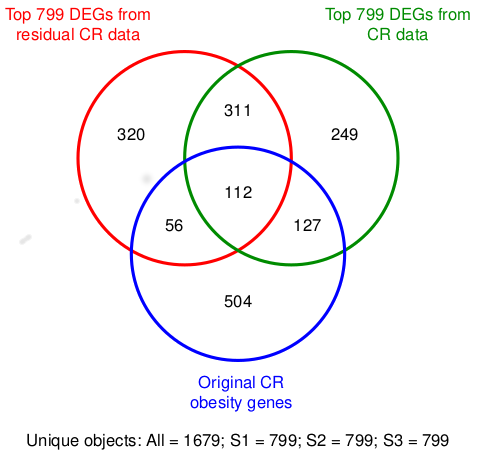
\includegraphics[width=0.5\linewidth]{results1/deg_venn1}
	\caption[Veen diagram of the \glspl{deg} identified from CR data (all samples)]{Venn diagram showing the common genes between the signatures obtained from unadjusted and clinical variable-adjusted CR data and the original obesity associated genetic signature.}
	\label{fig:venn1}
\end{figure}

\noindent
There was a possible bias between different ethnic groups, where African American patients were more likely to be obese compared to the Caucasian patients (see \cref{ssub:creighton_study}).
Though ethnicity was controlled in the residual data, the effect of ethnicity on the data was completely removed to prevent any possibility of ethnicity influencing the analysis.
Therefore, the effect of ethnicity was completely removed by considering only the Caucasian patients in CR data, which left a total of 77 Caucasian patients in the data set.
With this Caucasian-only data set, obesity associated genetic signatures were identified as described above; first with unadjusted data, then with the data with clinical variables adjusted (except ethnicity, as it has already been controlled for by considering Caucasian samples only), and lastly the common genes with the original signature were identified.

2129 and 1558 gene probes were identified in the unadjusted and clinical variable-adjusted Caucasian patient data, respectively.
As before, the most significant 799 gene probes were selected from these gene probes.
There were 148 and 92 common gene probes with the original genetic signatures and unadjusted or clinical variable-adjusted Caucasian patient data set, respectively.
Again, Venn diagram was used to summarise the genes identified from the Caucasian patient data set (\cref{fig:venn2}).
\\

\begin{figure}[htp!]
	\centering
	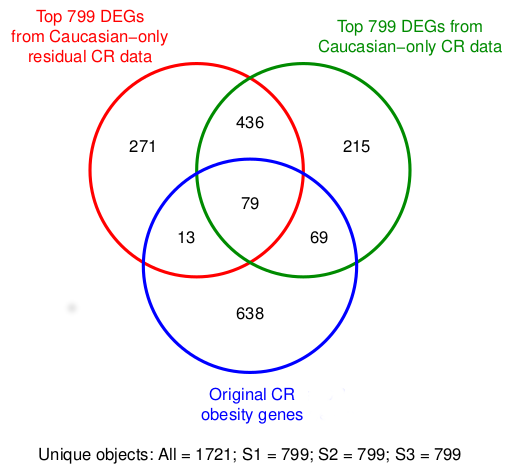
\includegraphics[width=0.5\linewidth]{results1/deg_venn2}
	\caption[Summary of the \glspl{deg} identified from CR data (Caucasian patient data)]{Venn diagram showing the common genes between the signatures obtained from unadjusted and clinical variable-adjusted CR data (Caucasian patients only) and the original obesity associated genetic signature.}
	\label{fig:venn2}
\end{figure}

\noindent
In addition to these eight obesity associated genetic signatures, a genetic signature was identified based on the correlation of gene probe expression with sample \gls{bmi} as continuous values, rather than discrete values as in \gls{bmi} status.
However, no significant genes were identified and thus was not used for further analysis (results detailed in appendix).

All of these obesity associated genetic signatures (eight in total) were checked to see whether these signatures had significant association with sample \gls{bmi}/\gls{bmi} status in various data set.
For simplicity, the abbreviations in \cref{tab:mg_abbrev} will be used to refer to the appropriate genetic signatures.

\begin{table}[htpb]
	\centering
	\caption{Summary of the abbreviations used to refer to the different obesity associated genetic signatures}
	\label{tab:mg_abbrev}
	\begin{tabular}{lp{0.51\textwidth}c}
		\hline
		\hline
		Abbreviation & Definition & No. of gene probes\\
		\hline
		\rule{0pt}{2.25ex}Or      & Original obesity associated genetic signature identified by \citet{Creighton2012}                       & 799\\
		\rule{0pt}{2.25ex}Cr      & Obesity associated genetic signature identified from unadjusted CR data                                & 799 \\
		\rule{0pt}{2.25ex}CrOl    & Genes common between Or and Cr genetic signatures                                                       & 239\\
		\rule{0pt}{2.25ex}Res     & Obesity associated genetic signature identified from clinical variable-adjusted CR data                & 799\\
		\rule{0pt}{2.25ex}ResOl   & Genes common between Or and Res genetic signatures                                                      & 168\\
		\rule{0pt}{2.25ex}Ca      & Obesity associated genetic signature identified from unadjusted Caucasian-only CR data                 & 799\\
		\rule{0pt}{2.25ex}CaOl    & Genes common between Or and Ca genetic signatures                                                       & 148\\
		\rule{0pt}{2.25ex}CaRes   & Obesity associated genetic signature identified from clinical variable-adjusted Caucasian-only CR data & 799\\
		\rule{0pt}{2.25ex}CaResOl & Genes common between Or and CaRes genetic signatures                                                    & 92\\
		\hline
		\hline
	\end{tabular}
\end{table}

\subsection{Novel obesity associated signatures and sample \gls{bmi}/\gls{bmi} status}
\label{sub:_novel_obesity_associated_signatures_and_sample_bmi}

As with the Or signature, all eight obesity associated genetic signatures were validated in CR data set first, and then compared in other cancer data sets by using the transformation matrix generated in CR data.
% Before the metagenes were created, all of the signatures were converted into gene symbols, as described in \cref{sec:data} (\cref{tab:signature_gene_num}).
CR data (unadjusted, all samples included) was normalised with \gls{rma} method and \gls{svd} was applied to generate the metagene for the corresponding genetic signature.
The direction of the metagenes were first examined to make sure that all of the metagenes were in line with one another (see \cref{sub:metagene_direction}; results shown in appendix).
The comparison of the metagenes with the sample gene expression in CR data were displayed as heatmaps (\cref{fig:degmetacr}).
It was clear from the heatmaps that all of the metagenes reflected the overall expression of the corresponding genetic signatures.
The association of the metagenes with sample \gls{bmi}/\gls{bmi} status was significant for all eight of the metagenes identified (\cref{fig:degmetacr}).
These results confirmed that all of the obesity associated genetic signatures identified in \cref{sub:identification_of_obesity_associated_genetic_signatures} significantly associated with sample \gls{bmi}/\gls{bmi} status in CR data, where the metagenes were derived from.

\begin{figure}[htp!]
	\centering
	\includegraphics[page=3,width=0.8\linewidth]{results1/cr_deg_meta_vs_clin}\\
	\vspace{1em}
	\includegraphics[page=4,width=0.45\linewidth]{results1/cr_deg_meta_vs_clin}
	\hfill
	\includegraphics[page=5,width=0.45\linewidth]{results1/cr_deg_meta_vs_clin}
	\caption[Cr obesity associated metagene in CR data]{Heatmap, box plot and scatter plot showing the association of Cr obesity associated metagene with sample gene expression, \gls{bmi} and \gls{bmi} status from CR data, respectively.
	The results for other metagenes are in \cref{app:a}.
	Scales, p-values and $R^2$-value are as described in previous figures.}
	\label{fig:degmetacr}
\end{figure}

Additionally, the correlation of all of the obesity associated metagenes were examined to see whether these metagenes were similar to one another.
As clearly shown in \cref{fig:cr_meta_cor}, there were two distinct groups within the eight metagenes; the first group contained the metagenes that were not overlapped with the Or metagene (Cr, Res, Ca and CaRes), while the other group had the overlapped metagenes (CrOl, ResOl, CaOl and CaResOl).
With that said, all eight metagenes showed high correlation with one another (lowest correlation approximately at 0.85), which suggested that all of these metagenes were detecting similar underlying biological mechanism from the data.

\begin{figure}[htpb]
	\centering
	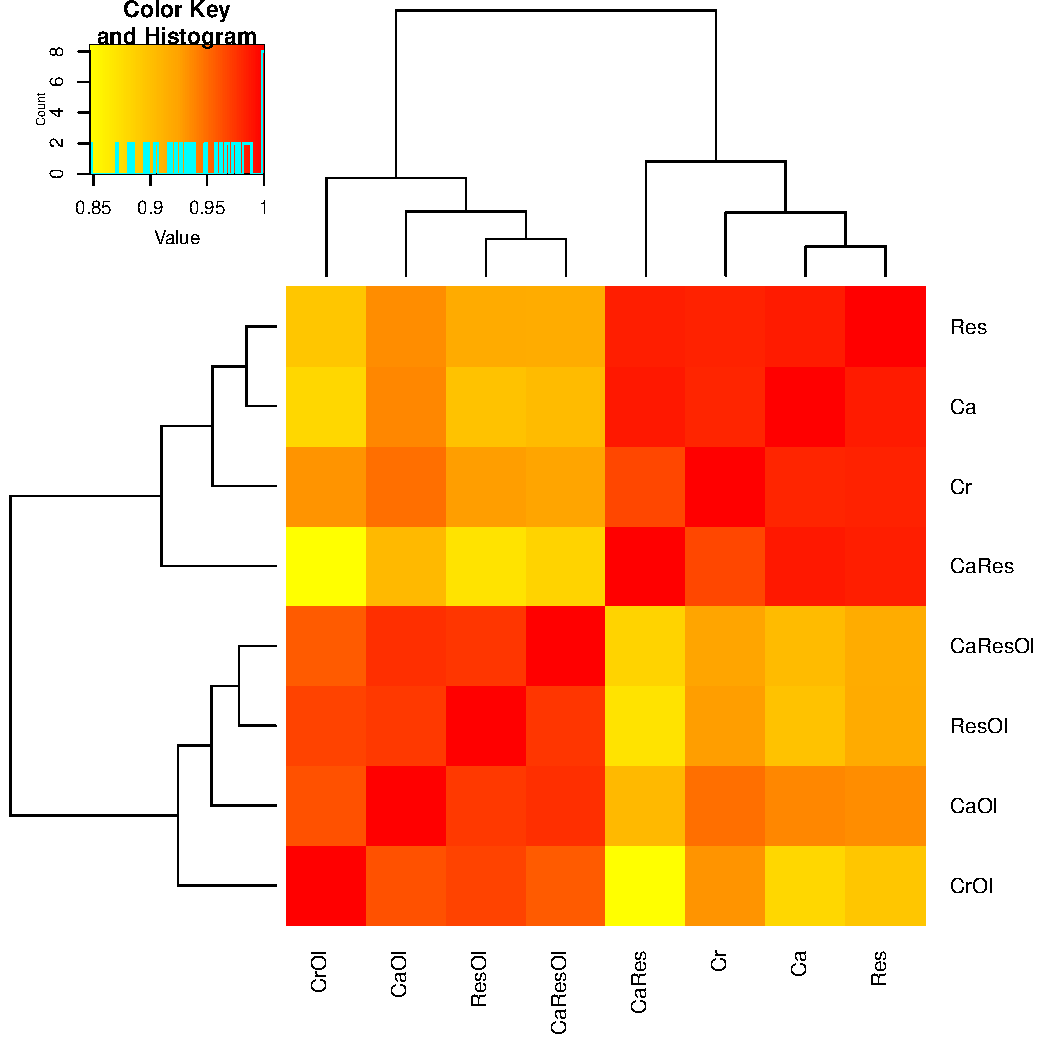
\includegraphics[width=0.8\linewidth]{results1/cr_meta_cor}
	\caption[Pearson correlation of all eight obesity associated metagenes identified in CR data]{Heatmap showing the Pearson correlation of all eight obesity associated metagenes from CR data with one another.
	\gls{svd} was applied to \gls{rma}-normalised CR data to generate each of the eight metagenes.
	High and low correlation were represented as red and blue, respectively, where the colours were matched with the values on the scale shown in top right.}
	\label{fig:cr_meta_cor}
\end{figure}

To confirm whether these metagenes showed significant association with sample \gls{bmi}/\gls{bmi} status in other cancer data sets, transformation matrix was applied to the \gls{icgc} cancer data and \gls{nzbc} data.
Firstly in \gls{icgc} cancer data sets, all eight metagene scores were reflective of the sample gene expression of the genetic signatures (\cref{fig:degmetaicgc}).
In all cancer types but \gls{blca}, none of the metagenes significantly associated with the sample \gls{bmi}/\gls{bmi} status (results shown in \cref{app:a}).
As shown in \cref{fig:degmetaicgc}, only the \gls{blca} data set showed significant association of the Cr metagene with sample \gls{bmi}/\gls{bmi} status.
With the metagenes other than Cr metagene, Res, CrOl and Ca metagenes showed statistical significance in overweight group, \gls{anova} and the regression line p-values; CaRes metagene was significant in overweight group and \gls{anova} p-value; CrOl and ResOl metagenes were significant in overweight group; and ResOl and CaOl metagenes were not significant in \gls{blca} data set.

This was unexpected since all of the genetic signatures were results of gene expression analysis between the non-obese group and the obese group of samples in CR data, and yet the metagenes showed significant association with the overweight group in \gls{blca} data set.
These results suggested that the samples that were overweight in \gls{blca} data were similar in phenotype with the samples that were obese in CR data.
Again, due to the fact that all of the metagenes lacked association with sample \gls{bmi}/\gls{bmi} status in all other \gls{icgc} data set, it was difficult to conclude whether the observed association of many of the obesity metagenes with the overweight group of samples was truly reflective of the effect resulted from these metagenes.

\begin{table}[htpb]
	\centering
	\caption{Statistics of all the obesity metagenes in \gls{blca} cancer data}
	\label{tab:degmetablca}
	\begin{threeparttable}
		\begin{tabular}{lccccc}
			& \multicolumn{3}{c}{ P-values} & \multicolumn{2}{c}{ Regression line statistics}\\
			\cmidrule(r){2-4} \cmidrule(r){5-6}
			 Metagenes &  Overweight &  Obese &  \gls{anova} &  R$^2$ &  P \\
			\hline
			\hline
			\rule{0pt}{2.25ex}Cr & {\bfseries 0.0134}\tnote{1} & 0.1365 & {\bfseries 0.0387} & 0.0171 & {\bfseries 0.0195} \\
			Res                  & {\bfseries 0.0055}          & 0.1974 & {\bfseries 0.0196} & 0.0117 & {\bfseries 0.0446} \\
			CrOl                 & {\bfseries 0.0383}          & 0.4583 & 0.1096             & 0.0047 & 0.1374             \\
			ResOl                & 0.0909                      & 0.7092 & 0.2125             & 0.0018 & 0.2254             \\
			Ca                   & {\bfseries 0.0077}          & 0.1973 & {\bfseries 0.0231} & 0.0116 & {\bfseries 0.0456} \\
			CaRes                & {\bfseries 0.0104}          & 0.2712 & {\bfseries 0.0322} & 0.0101 & 0.0572             \\
			CaOl                 & 0.0575                      & 0.6185 & 0.1487             & 0.0022 & 0.2126             \\
			CaResOl              & {\bfseries 0.0463}          & 0.5820 & 0.1263             & 0.0036 & 0.1660             \\
			\hline
			\hline
		\end{tabular}
		\begin{tablenotes}
			\item [1] All values in bold are statistically significant (p \textless{} 0.05).
		\end{tablenotes}
	\end{threeparttable}
\end{table}

In \gls{nzbc} data, the higher the metagenes scores were the more expressed the genes were (and vice versa), but lacked the association with sample \gls{bmi}/\gls{bmi} status (\cref{fig:degmetaprint}).
These results showed that, even though all of the metagenes significantly associated with sample \gls{bmi}/\gls{bmi} status in the data the genetic signatures were derived from, the metagenes did not transfer well in other cancer data sets.
Furthermore, these results showed that the lack of association with sample \gls{bmi}/\gls{bmi} status were not due to other clinical variables in CR data set.
This raised a question of whether there was any obesity associated genetic signature that was common in multiple cancer types.

\begin{figure}[htp!]
	\centering
	\includegraphics[page=3,width=0.8\linewidth]{results1/rawobsgene_ICGC}\\
	\vspace{1em}
	\includegraphics[page=4,width=0.45\linewidth]{results1/rawobsgene_ICGC}
	\hfill
	\includegraphics[page=5,width=0.45\linewidth]{results1/rawobsgene_ICGC}
	\caption[Cr obesity associated metagene in \acrshort{icgc} \acrshort{blca} data]{Heatmap, box plot and scatter plot showing the association of Cr obesity associated metagene with sample gene expression, \gls{bmi} and \gls{bmi} status from \acrshort{icgc} \acrshort{blca} data, respectively.
	The results for other metagenes and other cancer types are in \cref{app:a}.
	Scales, p-values and $R^2$-value are as described in previous figures.}
	\label{fig:degmetaicgc}
\end{figure}

\begin{figure}[htp!]
	\centering
	\includegraphics[page=3,width=0.8\linewidth]{results1/cris_crdeg_trans_meta}\\
	\vspace{1em}
	\includegraphics[page=4,width=0.45\linewidth]{results1/cris_crdeg_trans_meta}
	\hfill
	\includegraphics[page=5,width=0.45\linewidth]{results1/cris_crdeg_trans_meta}
	\caption[Cr obesity associated metagene in \gls{nzbc} data]{Heatmap, box plot and scatter plot showing the association of Cr obesity associated metagene with sample gene expression, \gls{bmi} and \gls{bmi} status from \gls{nzbc} data, respectively.
	The results for other metagenes are in \cref{app:a}.
	Scales, p-values and $R^2$-value are as described in previous figures.}
	\label{fig:degmetaprint}
\end{figure}

\section{Common genes across multiple cancer types}
\label{sec:common_genes_across_multiple_cancer_types}

It was clear that the obesity associated genetic signatures created from CR data were not consistent across different data sets.
To determine whether there was any obesity associated genetic signature that was expressed in multiple different cancer types, gene expression analysis was carried out on each of the eight \gls{icgc} cancer types and common genes were searched from the \glspl{deg} that were identified.
All of the \gls{icgc} cancer data sets were normalised with voom method (\cref{ssub:rna_seq_data}), which were then put through the gene expression analysis pipeline to identify \glspl{deg} between the obese group of samples and non-obese group of samples (\cref{sec:gene_expression_analysis}).
\cref{tab:icgcdegnum} summarised the number of genes found from each cancer type with p \textless{} 0.05.

\begin{table}[htbp]
	\centering
	\caption{Summary of the number of \glspl{deg} identified in each \gls{icgc} cancer data set}
	\label{tab:icgcdegnum}
	\begin{tabular}{lc}
		Cancer type & No. of \glspl{deg} identified\\
		\hline
		\hline
		\rule{0pt}{2.25ex}\gls{blca} & 679 \\
		\gls{cesc} & 1229\\
		\gls{coad} & 974\\
		\gls{kirp} & 687\\
		\gls{lihc} & 3340\\
		\gls{read} & 796\\
		\gls{skcm} & 1137\\
		\gls{ucec} & 2934\\
		\hline
		\hline
	\end{tabular}
\end{table}

There were 9695 unique \glspl{deg} across the eight cancer types, and these genes were checked for any commonalities across the different cancer types.
There were 7330 genes that were differentially expressed by one cancer type, 2024 genes expressed by any two cancer types, 320 genes expressed by any three cancer types, and 21 genes expressed by any four cancer types.
There were no genes differentially expressed by six or more cancer types (see \cref{tab:icgcdegtab} for a summary).
To confirm that these results were statistically significant, the gene expression analysis was repeated 1000 times for each cancer type after the samples were randomised in each analysis (see \cref{sub:sample_randomisation_in_simulation_analysis}).
The results from the simulation were summarised together with the earlier results in \cref{tab:icgcdegtab}.

The results from the simulation showed that, on average, 5732 genes were found to be differentially expressed by a cancer type, 1057 by two cancer types, 111 by three cancer types, and 7 by four cancer types.
When the results from \gls{icgc} gene expression analysis were compared with the simulation results, the number of \glspl{deg} found were statistically significant, as the numbers of genes identified exceeded the 95$^{th}$ percentile values for up to 5 cancer types.
This result confirmed that the \glspl{deg} from the \gls{icgc} cancer data were not identified by chance.
Unfortunately, there were no \glspl{deg} expressed in all eight cancer types, which confirmed that there was no common genes that were differentially expressed between the samples that were obese and normal weight.

\begin{table}[htbp]
	\centering
	\begin{threeparttable}
		\caption{Summary of the number of \glspl{deg} identified by the gene expression analysis and simulation analysis in \gls{icgc} cancer data}
		\label{tab:icgcdegtab}
		\begin{tabular}{>{\quad}lcccccccc}
			& \multicolumn{8}{c}{\small No. of cancer types expressing the \glspl{deg}\tnote{1}}\\
			& 1 & 2 & 3 & 4 & 5 & 6 & 7 & 8\\
			\hline
			\hline
			\rule{0pt}{2.25ex}\hspace{-1em}{\small Results from gene expression analysis} & 7330 & 2024 & 320 & 21 & 0 & 0 & 0 & 0 \\
			\hspace{-1em}{\small Results from simulation:\tnote{2}}                       &      &      &     &    &   &   &   &   \\
			{\small Mean no. of \glspl{deg} identified}                                   & 5732 & 1057 & 111 & 7  & 0 & 0 & 0 & 0 \\
			{\small $95^{th}$ percentile}                                                 & 6965 & 1722 & 227 & 20 & 2 & 0 & 0 & 0 \\
			\hline
			\hline
		\end{tabular}
		\begin{tablenotes}
			\begin{footnotesize}
			\item [1] The numbers represent the number of cancer types a gene was expressed in.
			\item [2] The simulation was repeated 1000 times, each with randomised samples.
			\end{footnotesize}
		\end{tablenotes}
	\end{threeparttable}
\end{table}

\section{Pathways enriched in \gls{icgc} data sets}
\label{sec:pathways_enriched_in_icgc_data_sets}

To check whether there were any significant pathways enriched in any of the \gls{icgc} cancer data sets that were associated with obesity, pathway enrichment analysis was carried out on each cancer type separately and then all cancer types combined (\cref{sec:pathway_enrichment_analysis}).
Each cancer type was normalised with voom (\cref{ssub:rna_seq_data}) and pathway enrichment analysis was carried out as described in \cref{sec:pathway_enrichment_analysis}.
Unfortunately, there were no pathways significantly enriched in any of the \gls{icgc} cancer types when analysed independent of one another.

Since there were no pathways enriched in any of the cancer types when analysed individually, all of the \gls{icgc} cancer data sets were combined to see if there were any pathways enriched in the combined data set.
The combined data set was generated in two ways: first combined data set was created by voom normalising each cancer data set separately, combine all of the normalised cancer data sets into one, then applied batch correction to the data set (\cref{sub:batch_correction}); and the second combined data set was created by combining the cancer data sets into one first, then the combined data was voom normalised, and finally batch correction was applied to obtain the final data set.
Each of the combined data sets were analysed for enriched pathways, but there were no pathways significantly enriched in either data sets.
These results suggested that there were no biological pathways associated with obesity in the \gls{icgc} cancer data sets.



\chapter{Obesity associated genetic signatures and pathway signatures}
\label{cha:obesity_associated_genetic_signature_and_pathway_signatures}

In this chapter, the underlying biological mechanism of the obesity associated signatures from the CR data were investigated.
In doing so, the pathway genetic signatures from the \citet{Gatza2010a} study (GT) were utilised to determine which biological pathways the obesity associated genetic signatures were most similar to.
First, the direction of GT pathway associated genetic signatures were resolved, then the pathway associated metagenes were compared with the obesity associated metagenes, and lastly linear models were constructed based on the pathway metagenes and patient \gls{bmi} to predict the obesity associated metagenes.

\section{Pathway associated genetic signatures from \citet{Gatza2010a} study}
\label{sec:pathway_associated_genetic_signatures_from_gatza2010a_study}

\subsection{Ranking and normalisation methods for pathway metagenes}
\label{sub:ranking_and_normalisation_methods}

In the \citet{Gatza2010a} study, their data comprised of samples from different studies which were aggregated into a single data set that was \gls{mas} normalised, and the metagene scores were transformed to a scale between 0 to 1 using a probit function.
However, the analyses so far have used the \gls{rma} normalisation method and ranked based on the number of samples present in the data (fractional ranking; \cref{sub:ranking_of_the_metagene_scores}).
To decide which normalisation methods or ranking approaches were suitable for the analysis, the different methods were compared in the GT data (\cref{sec:ranking_method_for_the_pathway_associated_genetic_signatures,sec:normalisation_method_for_pathway_associated_genetic_signature_transformation_matrices}).
Results shown in \cref{sec:ranking_method_for_the_pathway_associated_genetic_signatures} clarified that there was no substantive difference in the ranking approaches used.

Scatter plots were generated and the correlations were calculated for each of the GT pathway metagenes derived from either \gls{rma} or \gls{mas} normalised GT data (\cref{sec:normalisation_method_for_pathway_associated_genetic_signature_transformation_matrices}).
The GT pathway metagenes were generated using the transformation matrices that were derived from either the \gls{rma} or \gls{mas} normalised GT data.
From these results, it was clear the normalisation methods used on the data set had the most significant effect on the resulting metagenes, rather than the normalisation methods used to generate the transformation matrices (\cref{sec:normalisation_method_for_pathway_associated_genetic_signature_transformation_matrices}).
This meant that all of the data sets had to be normalised with a single normalisation method, so \gls{rma} was chosen as the normalisation method to be used as this method is regarded as being more reliable than the \gls{mas} method \citep{Irizarry2003}.

Another thing noted from these scatter plots was that there were some pathway signatures that were more variable than the others (\cref{sec:normalisation_method_for_pathway_associated_genetic_signature_transformation_matrices}).
As an example, the \gls{tgfb} metagenes were significantly more dispersed compared to the \gls{pr} metagenes, even though both of these metagenes were generated in the same data set through similar processes (\cref{fig:gt_rma_vs_mas}).
These differences were seen in other data sets as well (\cref{fig:appendix/gt_meta_rma_mas_other_data}).
This result provided evidence that some of the pathway genetic signatures from the \citet{Gatza2010a} study were less variable across different data sets than the others.
Taken together, it was decided that the GT data set should be batch corrected first (\cref{sub:batch_correction}), then normalised with the \gls{rma} method, and the metagene scores were ranked with fractional ranking (\cref{sub:ranking_of_the_metagene_scores}).

\begin{figure}[htpb]
	\centering
	\includegraphics[page=76,width=0.45\linewidth]{results2/allmeta_rma_vs_mas}
	\includegraphics[page=100,width=0.45\linewidth]{results2/allmeta_rma_vs_mas}
	\caption[Comparison of the pathway metagenes generated in the \acrshort{mas} normalised GT data set from the application of the transformation matrices derived from either the \acrshort{rma} or \acrshort{mas} normalised GT data]{Comparison of the pathway metagenes generated in the \acrshort{mas} normalised GT data set from the application of the transformation matrices derived from either the \acrshort{rma} or \acrshort{mas} normalised GT data.
	Only the \gls{pr} (left) and the \gls{tgfb}  (right) pathway metagenes are shown.
	The scatter plots for the other pathway metagenes are shown in \cref{sec:normalisation_method_for_pathway_associated_genetic_signature_transformation_matrices}.
	}
	\label{fig:gt_rma_vs_mas}
\end{figure}

\subsection{Pathway metagene directionality}
\label{sub:pathway_metagene_directionality}

Before GT pathway metagenes were compared with the obesity associated metagenes, the direction of the GT pathway metagenes had to be checked to make sure that the metagenes were in the ``correct'' direction (\cref{sub:metagene_direction}).
The correlation of all the pathway metagenes with one another were plotted as a heatmap in \cref{fig:gatza_meta_dir}.
The most prominent group had five pathways (E2F1, \gls{pi3k}, Myc, \gls{bcat} and Ras) that clustered at the top right hand corner of the heatmap.
Other groups included \gls{ifna}/\gls{ifny}/\gls{tnfa} pathways, \gls{er}/\gls{pr}/p53 pathways and p63/\gls{her2} pathways.
In addition to these highly correlated groups, \gls{stat3}/\gls{tgfb}/Src/\gls{egfr}/Akt pathways showed little correlation with one another.
Comparing these groups with the results presented by \citet{Gatza2010a} (\cref{sec:result_from_gatza2010a_study}), the identified clusters approximately resembled the pathway groups identified in by Gatza \textit{et al.}, which confirmed that the directions of GT pathway metagenes were consistent with those used by Gatza \textit{et al.}.

\begin{figure}[htpb]
	\centering
	\includegraphics[page=15,width=0.7\linewidth]{results2/gatza_meta_trans}
	\caption[Heatmap of the Pearson correlation of all the pathway metagenes with one another in the \acrshort{rma} normalised GT data]{Heatmap showing the Pearson correlation of all the pathway metagenes from the \citet{Gatza2010a} study with one another  in the \gls{rma} normalised GT data set.
		High and low correlation were represented as red and blue, respectively, where the colours were matched with the values on the scale shown in the top left histogram.
		Refer to \cref{tab:metagene_direction} for the detailed descriptions of the abbreviations used.
		}
	\label{fig:gatza_meta_dir}
\end{figure}

To see whether the directionality of the GT pathway metagenes were being transferred across to other data sets properly, pathway metagenes were generated in other data sets with the same transformation matrices and the groupings of the metagenes were examined.
CR, FM and \gls{nzbc} data were \gls{rma} normalised and transformation matrices of the pathway genetic signatures (derived from the GT data set) were applied to the data sets.
The metagenes were plotted in a heatmap (shown in \cref{sec:correlation_of_the_gt_pathway_metagenes_in_other_cancer_data_sets}), which showed similar groupings  as seen in \cref{fig:gatza_meta_dir}.
This result confirmed that the pathway metagenes were acting similarly in all of the data sets in which the transformation matrices have been applied to.

\section{Pathway associated metagenes and obesity associated metagenes}
\label{sec:pathway_associated_metagenes_and_obesity_associated_metagenes}

Results from the previous section confirmed that the pathway metagenes from the \citet{Gatza2010a} study were in the correct directions, and that the pathway metagenes were behaving as expected in the different data sets.
Now that the directions of the pathway metagenes were established, these metagenes were ready for comparison with the obesity associated metagenes.
However, all of the pathway metagenes were derived from the GT data, whereas the majority of the obesity associated metagenes were derived from the CR data, which presents a problem in terms of deciding which data set the transformation matrices should be generated in.

\subsection{Obesity and pathway metagene transformation matrices}
\label{sub:obesity_and_pathway_metagene_transformation_matrices}

Metagenes generated from the application of \gls{svd} and metagenes generated from the transformation matrix are exactly the same if the transformation matrix is derived from the same data set.
For example, an obesity associated metagene generated from the CR data with \gls{svd} would have the same values as the metagenes generated in the CR data with the transformation matrix (where the transformation matrix was derived from CR data).
Furthermore, if the \gls{svd}-derived metagenes and transformation matrix-derived metagenes were the same (or at least similar) in a different data set, this suggests that the metagene-related biology contained in the two data sets is highly similar.
In other words, the transformation matrix can be made in either the original data set or in a different data set if there was no difference in the \gls{svd}-derived or transformation matrix-derived metagenes.

To decide which data set the transformation matrices for obesity and pathway associated genetic signatures should be generated in, the \gls{svd}- and transformation matrix(TM)-generated metagene scores were compared in all of the data sets.
As in \cref{sec:pathway_associated_genetic_signatures_from_gatza2010a_study}, all data sets were normalised with the \gls{rma} method and metagenes were ranked with fractional ranking.
TMs for the obesity associated genetic signatures were made in the CR data set and the TMs for pathway associated genetic signatures were made in the GT data set.
Metagenes for all of the obesity and pathway associated genetic signatures were generated in all of the data sets with \gls{svd} and TMs.
The Spearman correlation of the \gls{svd}-generated and TM-generated metagene scores were calculated for each genetic signatures (\cref{tab:svd_vs_tm_path,tab:svd_vs_tm_obs}).

\begin{table}[htpb]
	\centering
	\begin{threeparttable}
	\caption[Summary of the Spearman correlations of the \gls{svd}- and TM-derived pathway metagenes in the GT, CR, \gls{nzbc} and FM data sets]{Summary of the Spearman correlations of the \gls{svd}- and transformation matrix\tnote{1}-derived pathway metagenes in the GT, CR, \gls{nzbc} and FM data sets}
	\label{tab:svd_vs_tm_path}
		\begin{tabular}{lcccc}
			& GT & CR & \gls{nzbc} & FM\\
			\hline
			\hline
			\rule{0pt}{2.25ex}Akt & 1.000 & 0.5190 & 0.5900 & 0.5563 \\
			\gls{bcat}            & 1.000 & 0.9897 & 0.9977 & 0.9905 \\
			E2F1                  & 1.000 & 0.9646 & 0.8438 & 0.9193 \\
			\gls{egfr}            & 1.000 & 0.0430 & 0.3358 & 0.4040 \\
			\gls{er}              & 1.000 & 0.9978 & 0.9942 & 0.9966 \\
			\gls{her2}            & 1.000 & 0.9553 & 0.5817 & 0.9794 \\
			\gls{ifna}            & 1.000 & 0.9830 & 0.9991 & 0.9951 \\
			\gls{ifny}            & 1.000 & 0.9086 & 0.9950 & 0.9718 \\
			Myc                   & 1.000 & 0.9878 & 0.9852 & 0.9689 \\
			p53                   & 1.000 & 0.3808 & 0.9981 & 0.7923 \\
			p63                   & 1.000 & 0.8319 & 0.2951 & 0.8368 \\
			\gls{pi3k}            & 1.000 & 0.9543 & 0.5989 & 0.9365 \\
			\gls{pr}              & 1.000 & 0.9511 & 0.9887 & 0.9845 \\
			Ras                   & 1.000 & 0.9078 & 0.9125 & 0.7229 \\
			Src                   & 1.000 & 0.9575 & 0.7173 & 0.9548 \\
			\gls{stat3}           & 1.000 & 0.1902 & 0.9159 & 0.6167 \\
			\gls{tgfb}            & 1.000 & 0.9918 & 0.2543 & 0.9890 \\
			\gls{tnfa}            & 1.000 & 0.6046 & 0.9365 & 0.4315 \\
			\hline
			\hline
		\end{tabular}
		\begin{tablenotes}
			\begin{footnotesize}
				\item [1] Transformation matrices were derived from the \gls{rma} normalised GT data set.
			\end{footnotesize}
		\end{tablenotes}
	\end{threeparttable}
\end{table}

\begin{table}[htpb]
	\centering
	\begin{threeparttable}
	\caption[Summary of the Spearman correlations of the \gls{svd}- and TM-derived obesity metagenes in the GT, CR, \gls{nzbc} and FM data sets]{Summary of the Spearman correlations of the \gls{svd}- and transformation matrix\tnote{1}-derived obesity metagenes in the GT, CR, \gls{nzbc} and FM data sets}
		\label{tab:svd_vs_tm_obs}
		\begin{tabular}{lcccc}
			& CR & GT & FM & \gls{nzbc}\\
			\hline
			\hline
			\rule{0pt}{2.25ex} Cr & 1.000     & 0.9985 & 0.9872 & 0.9161 \\
			Res                   & 1.000     & 0.9987 & 0.9898 & 0.9652 \\
			CrOl                  & 1.000     & 0.9982 & 0.9926 & 0.9715 \\
			ResOl                 & 1.000     & 0.9981 & 0.9927 & 0.9571 \\
			Ca                    & 1.000     & 0.9985 & 0.9893 & 0.9468 \\
			CaRes                 & 1.000     & 0.9988 & 0.9939 & 0.9865 \\
			CaOl                  & 1.000     & 0.9983 & 0.9937 & 0.9677 \\
			CaResOl               & 1.000     & 0.9984 & 0.9952 & 0.9642 \\
			Original              & 1.000     & 0.9928 & 0.9862 & 0.9344 \\
			\hline
			\hline
		\end{tabular}
			\begin{tablenotes}
				\begin{footnotesize}
				\item [1] Transformation matrices were derived from the \gls{rma} normalised CR data set.
				\end{footnotesize}
			\end{tablenotes}
	\end{threeparttable}
\end{table}

In \cref{tab:svd_vs_tm_path,tab:svd_vs_tm_obs}, the obesity and pathway associated genetic signatures had a correlation of 1 in CR and GT data sets respectively, as the obesity and pathway TMs were generated in the CR and GT data sets, respectively.
The correlations of the obesity and pathway metagenes were variable across different data sets, which was as expected since all the data sets were different from one another.
However, what was unexpected was the fact that there were some pathway genetic signatures that were highly correlated in all of the data sets, and there were others that varied considerably across different data sets.
For example, the \gls{bcat} pathway metagene was highly correlated in all of the data sets (\textgreater{} 0.98), whereas the \gls{stat3} pathway metagene was variable across different data sets, ranging from 0.1902 to 0.9159 (\cref{tab:svd_vs_tm_path}; \cref{sec:comparison_of_the_correlation_of_svd_and_tm_generated_pathway_metagenes}).
The fact that some pathway associated metagenes were consistent across different data sets suggested that some of these genetic signatures were reliable and did not depend on the data set the transformation matrices were derived from.
On the other hand, the genetic signatures that were not consistent across the data sets were likely to be dependent on the data set in which they were derived from, and therefore the transformation matrices for these signatures must be derived from the GT data set.
This also showed that the tumour biology may be different across the data sets, likely due to the difference in the patient cohorts that were selected for each of the studies.

In contrast to the pathway associated genetic signatures, all of the obesity associated genetic signatures showed high correlation for the \gls{svd}- and transformation matrix-generated metagenes across the different data sets.
This suggested that the obesity associated genetic signatures were relatively consistent across all data sets, and the transformation matrices for these signatures could be made in any of the data sets.
For simplicity, it was decided that the transformation matrices for all the genetic  signatures would be made in the GT data set, since there were some pathway associated signatures that were specific to the GT data.

\subsection{Comparison of the obesity and pathway associated signatures}
\label{sub:comparison_of_the_obesity_and_pathway_associated_signatures}

To visually determine which pathway associated genetic signatures were most similar to the obesity associated genetic signatures, heatmaps were created with the metagenes for all of the genetic signatures.
The directions of the pathway associated metagenes have already been determined in \cref{sec:pathway_associated_genetic_signatures_from_gatza2010a_study}, and the directions of the obesity associated metagenes were checked in GT data set as described in \cref{sub:metagene_direction}.
All of the metagenes were created in the GT data set (normalised with \gls{rma}) using \gls{svd}, and the metagene scores were plotted in a heatmap and clustered into groups (\cref{fig:gatza_allmeta}).

\begin{figure}[htpb]
	\centering
	\includegraphics[page=15,width=0.8\linewidth]{results2/all_meta_trans}
	\caption[Heatmap of the Pearson correlation of all the pathway and obesity metagenes with one another in the \acrshort{rma}-normalised GT data]{Heatmap showing the Pearson correlation of all the pathway and obesity metagenes  with one another  in the \gls{rma}-normalised GT data set.
		High and low correlation were represented as red and blue, respectively, where the colours were matched with the values on the scale shown in the top left histogram.
		Refer to \cref{tab:metagene_direction,tab:mg_abbrev} for the detailed descriptions of the abbreviations used.
		}
	\label{fig:gatza_allmeta}
\end{figure}

In \cref{fig:gatza_allmeta}, all of the obesity associated metagenes from the CR data set cluster together into a group, but none of the pathway associated metagenes had  a strong positive correlation with the obesity metagenes.
Though the  \gls{her2} and p63 pathway metagenes were grouped next to the cluster of obesity metagenes, the similarity was at most about 0.6  (Pearson correlation; \cref{fig:gatza_allmeta}).
With that said, these obesity associated metagenes seem to have a strong negative correlation with some of the pathway associated genetic signatures, such as the Akt, \gls{er}, \gls{egfr}, \gls{pr}, p53, Src and \gls{tgfb} pathways, and this strong negative correlation was observed in the other data sets as well (\cref{sec:correlation_of_the_pathway_and_obesity_metagenes_in_other_cancer_data_sets}).
In fact,  high Or metagene scores related to lower levels of gene expression for the genes in the Or signature (\cref{fig:crmetaheat}; \cref{sec:creighton_obesity_metagene}), and therefore it could be possible that many of the genes in the Or signature (and the other obesity associated signatures from the CR data) may be positively correlated with the genes in these pathway signatures.
This suggests that the obesity associated genetic signatures from the CR data may be related to these pathway signatures, rather than the obesity phenotype of the patients.

The FM obesity associated metagene did not cluster together with the obesity metagenes from the CR data set, nor with any of the other pathway metagenes.
The fact that the FM metagene did not cluster with any of the CR metagenes showed that the signals captures by the FM metagene was different from those metagenes found in the CR data set.
Furthermore, the FM metagene did not cluster with the Akt pathway in the heatmap, even though \citet{Fuentes-Mattei2014} provided clear evidence that their metagene specifically activated the Akt/\gls{mtor} signalling pathway in a mouse model.
This may have been due to the lack of consistency of the Akt pathway signature in the different data sets (\cref{tab:svd_vs_tm_path}).
Another likely reason could be that FM genetic signature was not comprised only of the genes from the Akt pathway, but genes from the other pathways as well, and so the metagene did not cluster together with the Akt pathway signature in the heatmap.

The results in this section suggested that none of the obesity associated genetic signatures were positively correlated with any of the pathway associated genetic signatures from the \citet{Gatza2010a} study.
However, some pathway signatures were negatively correlated with the obesity associated genetic signatures, which meant that the obesity signatures were likely capturing the signals from these signatures  rather than the biological signals from the obesity phenotype of the patient.

\section{Prediction of obesity associated metagenes with pathway associated metagenes}
\label{sec:prediction_of_obesity_associated_metagene_with_pathway_associate_metagene}

To confirm the biological relationship between the obesity associated metagenes with the pathway associated metagenes from the \citet{Gatza2010a} study, linear models were created to predict the obesity metagene scores with the pathway metagene scores.
If any of the pathway metagenes were significant in the linear model, this would provide evidence that the significant pathways in the linear model were related to the obesity metagene.
Since most of the obesity metagenes were found in the CR data set, and only the CR and the \gls{nzbc} data sets had \gls{bmi} information for the patients, \gls{nzbc} data set was used as the training data set to create the linear models for obesity metagene score prediction.

\subsection{Linear model prediction in the \gls{nzbc} and CR data sets}
\label{sub:linear_model_prediction_in_the_nzbc_and_cr_data_sets}

Metagene scores used for the construction of linear models were generated from the application of the transformation matrices derived from the GT data (from \cref{sec:pathway_associated_metagenes_and_obesity_associated_metagenes}) to \gls{rma} normalised \gls{nzbc} data.
From \cref{tab:svd_vs_tm_path}, it was evident that some pathway associated genetic signatures could be variable across different data sets.
Therefore, only six pathways (\gls{bcat}, \gls{er}, \gls{ifna}, \gls{ifny}, Myc and \gls{pr}) that were ``consistent'' (correlation \textgreater{} 0.9) across all of the data sets were used to construct the linear models.

For each of the obesity metagenes identified, seven linear models were created: \gls{bmi}-only, \gls{bmi} status-only, \gls{bmi} and \gls{bmi} status, pathway metagenes-only, and the combinations of pathway metagenes with \gls{bmi} and/or \gls{bmi} status.
The only variables that showed significance in any of the models that predicted the obesity metagenes taken from the CR data set were the \gls{pr} metagene and whether the patients were obese or not (\cref{tab:lm_sig_var}).
In the model that predicted the FM metagene scores, the obesity status of the patients and Myc metagene score were significant, but the \gls{pr} metagene score was not (\cref{sec:summary_of_the_linear_models_in_nzbc_data}).

\begin{table}[htpb]
	\centering
	\caption{Description of the linear models constructed from the \gls{nzbc} data to predict the Cr obesity metagene}
	\label{tab:lm_sig_var}
	\begin{threeparttable}
		\begin{tabular}{llrr}
			Linear Model & Variables & Estimate & P-value\\
			\hline
			\hline
			\rule{0pt}{2.25ex}\gls{bmi} only                           & \gls{bmi}  & -0.0016 & 0.717\\
			\hline
			\rule{0pt}{2.25ex}\gls{bmi} status only                    & Overweight & -0.0126 & 0.871\\
                                                                       & Obese      & -0.0981 & 0.166\\
			\hline
			\rule{0pt}{2.25ex}\gls{bmi} and \gls{bmi} status           & \gls{bmi}  & 0.0109  & 0.123\\
                                                                       & Overweight & -0.0687 & 0.420\\
                                                                       & Obese      & -0.2481 & \textbf{0.040}\tnote{1}\\
			\hline
			\rule{0pt}{2.25ex}Pathways only                            & \gls{bcat} & 0.0916  & 0.677\\
                                                                       & \gls{er}   & 0.0523  & 0.834\\
                                                                       & \gls{ifna} & -0.4993 & 0.307\\
                                                                       & \gls{ifny} & 0.4224  & 0.398\\
                                                                       & Myc        & -0.0038 & 0.987\\
                                                                       & \gls{pr}   & 0.5836  & \textbf{0.016}\\
			\hline
			\rule{0pt}{2.25ex}\gls{bmi} and Pathways                   & \gls{bmi}  & -0.0024 & 0.527\\
                                                                       & \gls{bcat} & 0.1121  & 0.614\\
                                                                       & \gls{er}   & 0.0540  & 0.829\\
                                                                       & \gls{ifna} & -0.5383 & 0.276\\
                                                                       & \gls{ifny} & 0.4661  & 0.358\\
                                                                       & Myc        & 0.0168  & 0.941\\
                                                                       & \gls{pr}   & 0.5927  & \textbf{0.015}\\
			\hline
			\rule{0pt}{2.25ex}\gls{bmi} status and Pathways            & Overweight & -0.0120 & 0.864\\
                                                                       & Obese      & -0.1035 & 0.113\\
                                                                       & \gls{bcat} & 0.1495  & 0.501\\
                                                                       & \gls{er}   & 0.0326  & 0.896\\
                                                                       & \gls{ifna} & -0.6707 & 0.177\\
                                                                       & \gls{ifny} & 0.5888  & 0.245\\
                                                                       & Myc        & 0.0439  & 0.846\\
                                                                       & \gls{pr}   & 0.5799  & \textbf{0.016}\\
			\hline
			\rule{0pt}{2.25ex}\gls{bmi}, \gls{bmi} status and pathways & \gls{bmi}  & 0.0091  & 0.161\\
                                                                       & Overweight & -0.0576 & 0.455\\
                                                                       & Obese      & -0.2292 & \textbf{0.040}\\
                                                                       & \gls{bcat} & 0.1460  & 0.509\\
                                                                       & \gls{er}   & 0.0091  & 0.971\\
                                                                       & \gls{ifna} & -0.6937 & 0.161\\
                                                                       & \gls{ifny} & 0.5890  & 0.243\\
                                                                       & Myc        & 0.0263  & 0.907\\
                                                                       & \gls{pr}   & 0.5449  & \textbf{0.024}\\
			\hline
			\hline
		\end{tabular}
		\begin{tablenotes}
			\begin{footnotesize}
				\item [1] All values in bold are statistically significant (p \textless{} 0.05).
			\end{footnotesize}
		\end{tablenotes}
	\end{threeparttable}
\end{table}

The models constructed from the patient \gls{bmi}, \gls{bmi} status and/or GT pathway metagene scores confirmed that none of the pathways were significant, except for the \gls{pr} and Myc pathway metagene scores in the models for the CR metagenes and the FM metagene, respectively.
It was not surprising that the \gls{pr} pathway metagene showed significance in the models generated in \gls{nzbc} data set, as majority of the patients in the \gls{nzbc} data set were \gls{pr}$^+$ (\cref{tab:clin_summary}).
The significance of the Myc metagene in the model for FM metagene was difficult to interpret, as there was no reported association of the FM metagene with the Myc pathway by \citet{Fuentes-Mattei2014}.
\textit{MYC} is an oncogene that encodes the Myc transcription factor that, when overexpressed, disrupts various pathways that directly promote tumour growth and proliferation, and has a central role in many of the cancer hallmarks \citep{Coller2000,Hanahan2000}.
``Sustained cell proliferation'' was one of the cancer hallmarks that \citet{Fuentes-Mattei2014} had shown to be related to their obesity associated genetic signature, which could be the reason that the Myc pathway metagene showed up as a significant variable in the linear model.

Since the \gls{pr} pathway metagene showed significant association in many of the linear models, linear models were made with each of the combinations of \gls{bmi}, \gls{bmi} status and \gls{pr} pathway metagene for all of the obesity associated metagenes (\cref{tab:lm_pr_only}; \cref{sec:summary_of_the_linear_models_in_nzbc_data}).
As expected, all of the linear models showed significant contribution of the \gls{pr} metagene scores to the model for all obesity metagenes (except FM metagene; \cref{sec:summary_of_the_linear_models_in_nzbc_data}).

\begin{table}[htpb]
	\centering
	\caption[Description of the linear models constructed from the \gls{nzbc} data to predict the Cr obesity, using only the patient \gls{bmi}, \gls{bmi} status and the \acrshort{pr} pathway metagene score]{Description of the linear models constructed from the \gls{nzbc} data to predict the Cr obesity, using only the patient \gls{bmi}, \gls{bmi} status and the \gls{pr} pathway metagene score}
	\label{tab:lm_pr_only}
	\begin{threeparttable}
			\begin{tabular}{llr{\bfseries}S}
				Linear Model & Variables & Estimate & {P-value}\\
				\hline
				\hline
				\rule{0pt}{2.25ex}\gls{pr} only                            & \gls{pr}   & 0.477  & {\bfseries \num{6.06d-7}}\tnote{1}\\
				\hline
				\rule{0pt}{2.25ex}\gls{bmi} and \gls{pr}                   & \gls{bmi}  & -0.002 & 0.586\\
                                                                           & \gls{pr}   & 0.478  & {\bfseries \num{6.35d-7}}\\
				\hline
				\rule{0pt}{2.25ex}\gls{bmi} status and \gls{pr}            & Obese      & -0.085 & 0.176\\
                                                                           & Overweight & -0.011 & 0.875\\
                                                                           & \gls{pr}   & 0.471  & {\bfseries \num{8.25d-7}}\\
				\hline
				\rule{0pt}{2.25ex}\gls{bmi}, \gls{bmi} status and \gls{pr} & \gls{bmi}  & 0.007  & 0.237\\
                                                                           & Obese      & -0.188 & 0.081\\
                                                                           & Overweight & -0.049 & 0.516\\
                                                                           & \gls{pr}   & 0.459  & {\bfseries \num{1.54d-6}}\\
				\hline
				\hline
			\end{tabular}
			\begin{tablenotes}
				\begin{footnotesize}
					\item [1] All values in bold are statistically significant (p \textless{} 0.05).
				\end{footnotesize}
			\end{tablenotes}
	\end{threeparttable}
\end{table}

To determine whether any of the linear models were able to predict the corresponding obesity metagene scores, the predicted metagene scores were generated from the models and then compared with the original scores.
The original obesity metagene scores from the \gls{nzbc} were generated from the application of TM that were derived from the \gls{rma}-normalised GT data set.
These \gls{nzbc} obesity metagene scores were then compared with the metagene scores that were predicted by the linear models (\cref{fig:predict_cris_cris}).

The predicted metagenes from all of the patient \gls{bmi}-related linear models were not significantly related to the original metagene scores in many of the obesity metagenes (\cref{fig:predict_cris_cris}; \cref{sec:summary_of_the_linear_models_in_nzbc_data}).
On the other hand, all of the predicted metagenes generated from the models that used the pathway metagene scores showed significant association with the original metagene scores (\cref{fig:predict_cris_cris}; \cref{sec:summary_of_the_linear_models_in_nzbc_data}).
However, the $R^2$ values for all of the predicted metagenes against the original metagenes were very low ($R^2$ \textless{} 0.4).
All of the plots in \cref{fig:predict_cris_cris,sec:summary_of_the_linear_models_in_nzbc_data} showed clearly that the data points in the scatter plots were highly variable, suggesting that even though the association between the predicted and the true metagene scores were statistically significant, the variables in the linear models may not be strongly associated to the obesity metagene.
Furthermore, the fact that all of the predictions made with the models that contained the \gls{pr} metagene showed greater correlation with the true metagene values suggested that most of the variations in the Cr (and other) obesity metagenes were being explained by the \gls{pr} metagene alone, and the patient \gls{bmi} contributed very little to the prediction.

\begin{figure}[htpb]
	\centering
	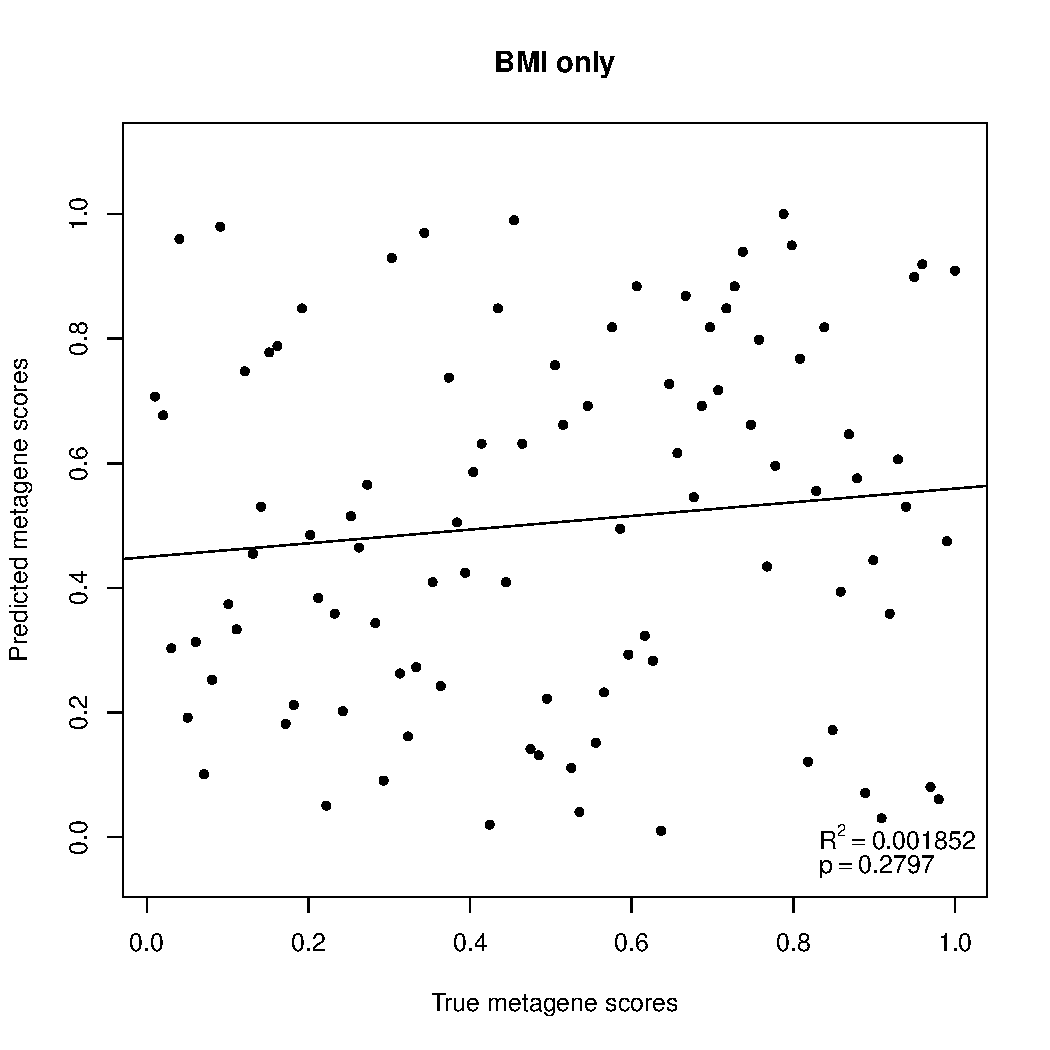
\includegraphics[page=1,width=0.32\linewidth]{results2/prediction_cris_with_cris(cris_model)}
	\includegraphics[page=2,width=0.32\linewidth]{results2/prediction_cris_with_cris(cris_model)}
	\includegraphics[page=3,width=0.32\linewidth]{results2/prediction_cris_with_cris(cris_model)}
	\includegraphics[page=4,width=0.32\linewidth]{results2/prediction_cris_with_cris(cris_model)}
	\includegraphics[page=5,width=0.32\linewidth]{results2/prediction_cris_with_cris(cris_model)}
	\includegraphics[page=6,width=0.32\linewidth]{results2/prediction_cris_with_cris(cris_model)}
	\includegraphics[page=7,width=0.32\linewidth]{results2/prediction_cris_with_cris(cris_model)}
	\includegraphics[page=74,width=0.32\linewidth]{results2/prediction_cris_with_cris(cris_model)}
	\includegraphics[page=71,width=0.32\linewidth]{results2/prediction_cris_with_cris(cris_model)}
	\includegraphics[page=72,width=0.32\linewidth]{results2/prediction_cris_with_cris(cris_model)}
	\includegraphics[page=73,width=0.32\linewidth]{results2/prediction_cris_with_cris(cris_model)}
	\caption[Comparison of the predicted Cr metagene scores with the Cr metagene score from the \gls{nzbc} data]{ Box plot and scatter plots comparing the Cr metagene score predicted by the different linear models constructed from the \gls{nzbc} data, with the Cr metagene score from the \gls{nzbc} data.
	Only the results from the models used to predict the Cr metagene scores are shown.
	The summary of the statistics for the other obesity metagene predictions from the \gls{nzbc} data are shown in \cref{sec:summary_statistics_of_the_predicted_obesity_metagenes_with_sample_bmi_bmi_status_in_nzbc_and_cr_data}.
	P-values and $R^2$-value are as described in previous figures.
	}
	\label{fig:predict_cris_cris}
\end{figure}

To confirm the results shown in the \gls{nzbc} data set (the training set), the linear models were applied to CR data (the test set).
As shown in \cref{fig:predict_cr_cris}, all of the predicted Cr metagene generated from the linear models were statistically significantly associated with the true Cr metagenes in CR data, but there were some exceptions in the models for the other obesity metagenes (\cref{sec:summary_statistics_of_the_predicted_obesity_metagenes_with_sample_bmi_bmi_status_in_nzbc_and_cr_data}).
Similar to the results from the \gls{nzbc} data set, all of the $R^2$ values were low ($R^2$ \textless{} 0.43) in the CR data set and the data points were widely spread out in the plots.
Again, these results suggested that the predicted metagene scores from the linear models may be statistically significant, but may not be relevant to the obesity metagenes which the models predict, as the predicted values were only weakly associated with the true values.

Another thing to note from \cref{fig:predict_cr_cris} was the apparent negative association of the predicted metagenes with the original metagenes in the \gls{bmi}-only, the \gls{bmi} status-only and the \gls{bmi} and \gls{bmi} status models.
One possible explanation for this was that these \gls{bmi}-based models were overfitted in the \gls{nzbc} data set, and was not generalisable in the CR data set, and thus produced negative correlations.
In fact, it was evident from the metagene analyses in \cref{cha:obesity_genetic_signatures_and_cancer} that these obesity associated genetic signatures were not generalisable with the patient \gls{bmi} in different data sets, and overfitting of the model in the \gls{nzbc} data was the likely cause of this negative correlation.

\begin{figure}[htpb]
	\centering
	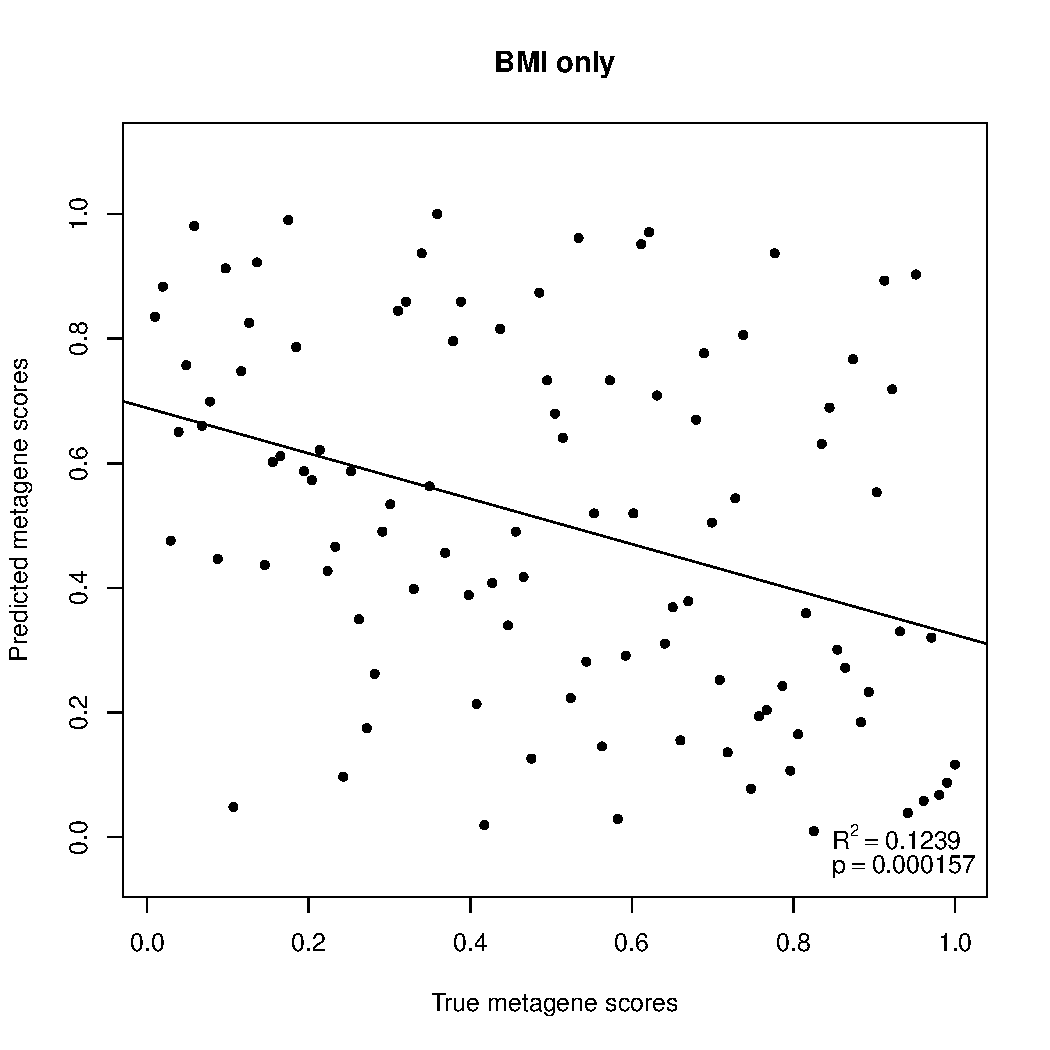
\includegraphics[page=1,width=0.32\linewidth]{results2/prediction_cr_with_cris}
	\includegraphics[page=2,width=0.32\linewidth]{results2/prediction_cr_with_cris}
	\includegraphics[page=3,width=0.32\linewidth]{results2/prediction_cr_with_cris}
	\includegraphics[page=4,width=0.32\linewidth]{results2/prediction_cr_with_cris}
	\includegraphics[page=5,width=0.32\linewidth]{results2/prediction_cr_with_cris}
	\includegraphics[page=6,width=0.32\linewidth]{results2/prediction_cr_with_cris}
	\includegraphics[page=7,width=0.32\linewidth]{results2/prediction_cr_with_cris}
	\includegraphics[page=74,width=0.32\linewidth]{results2/prediction_cr_with_cris}
	\includegraphics[page=71,width=0.32\linewidth]{results2/prediction_cr_with_cris}
	\includegraphics[page=72,width=0.32\linewidth]{results2/prediction_cr_with_cris}
	\includegraphics[page=73,width=0.32\linewidth]{results2/prediction_cr_with_cris}
	\caption[Comparison of the predicted Cr metagene scores with the Cr metagene score from the CR data]{ Box plot and scatter plots comparing the Cr metagene score predicted by the different linear models constructed from the \gls{nzbc} data, with the Cr metagene score from the CR data.
	Only the results from the models used to predict the Cr metagene scores are shown.
	The summary of the statistics for the other obesity metagene predictions from the CR data are shown in \cref{sec:summary_statistics_of_the_predicted_obesity_metagenes_with_sample_bmi_bmi_status_in_nzbc_and_cr_data}.
	P-values and $R^2$-value are as described in previous figures.
	}
	\label{fig:predict_cr_cris}
\end{figure}

\subsection{Stepwise linear model prediction in \gls{nzbc} and CR data sets}
\label{sub:stepwise_linear_model_prediction_in_nzbc_and_cr_data_sets}

Lastly, since only the six most ``consistent'' pathway metagenes were picked from a total of eighteen pathway metagene scores, linear models were constructed with all eighteen pathway metagenes in a stepwise fashion.
Step wise construction of a linear model is where the variables for a model are selected computationally depending on the contribution of the variable to the resulting linear model, and thus contain only the variables that ``matter'' to the final linear model \cref{sec:obesity_metagene_prediction_with_pathway_metagenes}.
Patient \gls{bmi}, \gls{bmi} status and all of the pathway metagenes (Akt, \gls{bcat}, E2F1, \gls{egfr}, \gls{er}, \gls{her2}, \gls{ifna}, \gls{ifny}, Myc, p53, p63, \gls{pi3k}, \gls{pr}, Ras, \gls{stat3}, Src, \gls{tgfb} and \gls{tnfa}) were used to generate the stepwise linear model for each of the obesity metagenes.
The linear models that resulted from the stepwise selection of the variables were summarised in \cref{tab:stepwise_model}.

These models were used to predict the obesity metagenes in the \gls{nzbc} data to test the performance of the models.
All of the models were able to make statistically significant prediction of the original obesity metagenes in the \gls{nzbc} data set (\cref{fig:stepwise_cris}).
Unlike the previous models, the stepwise models showed very high $R^2$ values, where most predictions had $R^2$ \textgreater{} 0.80.
The statistical significance and the strong association of the predicted metagenes were observed in the CR data set as well (\cref{fig:stepwise_cr}).
Though the $R^2$ values were slightly lower than those from the \gls{nzbc} data set, the $R^2$ values from the CR data predictions were more promising than the predictions made by the non-stepwise linear models.

\begin{ThreePartTable}
	\begin{TableNotes}
		\begin{footnotesize}
		\item [1] All values in bold are statistically significant (p \textless{} 0.05).
		\end{footnotesize}
	\end{TableNotes}
	\begin{longtable}{llr{\bfseries}S}
		\centering
		\caption[Description of the stepwise linear models constructed from the \gls{nzbc} data to predict all of the obesity metagenes]{Description of the stepwise linear models constructed from the \gls{nzbc} data to predict all of the obesity metagenes}
		\label{tab:stepwise_model}\\
			Obesity metagene & Variables retained in the model & Estimate & {P-value}\\
			\hline
		\endfirsthead
		\multicolumn{4}{c}{\tablename\ \thetable{}\ (continued)}\\
			\hline
			\hline
		\endhead
			\hline
			\hline
			Cr      & Src         & -0.1900  & \bfseries 0.005150\tnote{1}       \\
					& \gls{egfr}  & 0.1451   & \bfseries 0.002780                \\
					& \gls{tgfb}  & 0.5105   & \bfseries \num{1.17d-15}          \\
					& Akt         & -0.2821  & \bfseries \num{7.08d-06}          \\
					& \gls{ifna}  & -0.06968 & \bfseries 0.02986                 \\
			\hline
			CrOl    & Akt         & -0.3134  & \bfseries \num{1.76d-06}          \\
					& Src         & -0.5386  & \bfseries \textless{} \num{2d-16} \\
					& p53         & 0.3372   & \bfseries \num{9.18d-07}          \\
					& \gls{pr}    & -0.1115  & \bfseries 0.02760                 \\
			\hline
			Res     & \gls{tgfb}  & -0.5895  & \bfseries \num{1.53d-15}          \\
					& \gls{egfr}  & -0.3597  & \bfseries 0.0005390               \\
					& \gls{tnfa}  & 0.1604   & \bfseries 0.0006970               \\
					& \gls{bcat}  & -0.2141  & \bfseries 0.01157                 \\
					& Akt         & 0.1527   & \bfseries 0.02206                 \\
			\hline
			ResOl   & Akt         & -0.2802  & \bfseries 0.0001420               \\
					& Src         & -0.5214  & \bfseries \num{2.65d-15}          \\
					& p53         & 0.2861   & \bfseries \num{5.31d-07}          \\
			\hline
			Ca      & \gls{tgfb}  & 0.7470   & \bfseries \textless{} \num{2d-16} \\
					& Akt         & -0.2985  & \bfseries \num{2.83d-10}          \\
			\hline
			CaOl    & Src         & -0.5595  & \bfseries \num{3.88d-16}          \\
					& Akt         & -0.4331  & \bfseries \num{2.06d-11}          \\
			\hline
			CaRes   & \gls{tgfb}  & 0.7843   & \bfseries \textless{} \num{2d-16} \\
					& \gls{egfr}  & 0.2418   & \bfseries \num{2.19d-06}          \\
			\hline
			CaResOl & Src         & -0.4553  & \bfseries \num{1.57d-07}          \\
					& \gls{egfr}  & 0.2776   & \bfseries 0.0009570               \\
					& Akt         & -0.3001  & \bfseries 0.0001640               \\
					& E2F1        & 0.2484   & \bfseries 0.001300                \\
					& Myc         & 0.1584   & \bfseries 0.025220                \\
			\hline
			Or      & Src         & -0.5165  & \bfseries \textless{} \num{2d-16} \\
					& p53         & 0.3072   & \bfseries \num{2.60d-12}          \\
					& Akt         & -0.3006  & \bfseries 1.440e-07               \\
					& E2F1        & 0.09684  & \bfseries 0.01070                 \\
					& Obese       & -0.02190 & 0.2166                            \\
					& Overweight  & 0.03099  & 0.1223                            \\
			\hline
			FM      & p63         & 0.3507   & \bfseries 0.0006760               \\
					& \gls{stat3} & 0.2969   & \bfseries 0.004191                \\
					& p53         & 0.5368   & \bfseries 0.0008240               \\
					& \gls{pr}    & -0.3462  & \bfseries 0.034070                \\
			\hline
			\hline
			\insertTableNotes
	\end{longtable}
\end{ThreePartTable}

Clearly, the stepwise linear models were able to predict the obesity associated metagenes better than the models created in \cref{sub:linear_model_prediction_in_the_nzbc_and_cr_data_sets}.
This could be due to the fact that many of the stepwise linear models included many pathways that had a strong negative correlation with the obesity metagenes (Akt, \gls{er}, \gls{egfr}, \gls{pr}, p53, Src and \gls{tgfb} pathways; \cref{fig:gatza_allmeta}).
These pathway metagenes may have been better predictors of the obesity metagenes than the six pathways that were ``consistent'' across the data sets, and therefore generated better predictions than those linear models.
With that said, some of the predicted obesity metagenes from the stepwise linear models were negatively correlated with the original metagene values in the CR data (\cref{fig:stepwise_cr}).
Again, this could have been due to the model being overfit in the \gls{nzbc} data, and thus making an incorrect prediction about the obesity metagenes in the CR data.

\begin{figure}[htpb]
	\centering
	\includegraphics[page=1,width=0.32\linewidth]{results2/stepwise_cris_both_bic}
	\includegraphics[page=2,width=0.32\linewidth]{results2/stepwise_cris_both_bic}
	\includegraphics[page=3,width=0.32\linewidth]{results2/stepwise_cris_both_bic}
	\includegraphics[page=4,width=0.32\linewidth]{results2/stepwise_cris_both_bic}
	\includegraphics[page=5,width=0.32\linewidth]{results2/stepwise_cris_both_bic}
	\includegraphics[page=6,width=0.32\linewidth]{results2/stepwise_cris_both_bic}
	\includegraphics[page=7,width=0.32\linewidth]{results2/stepwise_cris_both_bic}
	\includegraphics[page=8,width=0.32\linewidth]{results2/stepwise_cris_both_bic}
	\includegraphics[page=9,width=0.32\linewidth]{results2/stepwise_cris_both_bic}
	\includegraphics[page=10,width=0.32\linewidth]{results2/stepwise_cris_both_bic}
	\caption[Comparison of all the obesity metagene scores predicted from the stepwise linear models with the original obesity metagene scores from the \gls{nzbc} data]{Scatter plots comparing all of the obesity metagene scores predicted by the stepwise linear models constructed from the \gls{nzbc} data, with the corresponding obesity metagene scores from the \gls{nzbc} data.
	P-values and $R^2$-value are as described in previous figures.}
	\label{fig:stepwise_cris}
\end{figure}

\begin{figure}[htpb]
	\centering
	\includegraphics[page=1,width=0.32\linewidth]{results2/stepwise_cr_both_bic}
	\includegraphics[page=2,width=0.32\linewidth]{results2/stepwise_cr_both_bic}
	\includegraphics[page=3,width=0.32\linewidth]{results2/stepwise_cr_both_bic}
	\includegraphics[page=4,width=0.32\linewidth]{results2/stepwise_cr_both_bic}
	\includegraphics[page=5,width=0.32\linewidth]{results2/stepwise_cr_both_bic}
	\includegraphics[page=6,width=0.32\linewidth]{results2/stepwise_cr_both_bic}
	\includegraphics[page=7,width=0.32\linewidth]{results2/stepwise_cr_both_bic}
	\includegraphics[page=8,width=0.32\linewidth]{results2/stepwise_cr_both_bic}
	\includegraphics[page=9,width=0.32\linewidth]{results2/stepwise_cr_both_bic}
	\includegraphics[page=10,width=0.32\linewidth]{results2/stepwise_cr_both_bic}
	\caption[Comparison of all the obesity metagene scores predicted from the stepwise linear models with the original obesity metagene scores from the CR data]{Scatter plots comparing all of the obesity metagene scores predicted by the stepwise linear models constructed from the \gls{nzbc} data, with the corresponding obesity metagene scores from the CR data.
	P-values and $R^2$-value are as described in previous figures.}
	\label{fig:stepwise_cr}
\end{figure}

Taken together, these results suggest that the variables included in these stepwise models were relevant to the biology of the obesity metagenes identified in the CR and FM data sets.
However, there were no common pathways that were present in all of the models; although Akt, \gls{egfr} and Src pathway metagenes were frequently included in many of the stepwise models.
The role of the pathways included in the models and the possible biological links of these pathways to the obesity metagenes remain unclear, and should be the focus for future investigations.



\chapter{Discussion (draft)}

\section{something}

% List of things to discuss

% RESULTS 1

% Creighton metagene section
% Lack of association of obesity metagenes with different cancer data sets
% -- due to metagene derivation from a specific data and therefore cannot be applied to other data set
% -- don't forget about the possibility of having samples that may not be driven by obesity at all in the data set (and therefore the metagene may be affected by these samples).

% FM metagene section
% -- don't forget about the possibility of having samples that may not be driven by obesity at all in the data set (and therefore the metagene may be affected by these samples).

% gene expression section
% -- mention that Creighton's group probably didn't control for FDR

\begin{figure}[ht]
\caption{Dummy}
\label{fig:dum1}
\end{figure}

\begin{table}[ht]
\caption{Dummy}
\begin{tabular}{|c|c|}
\end{tabular}
\label{tab:dum1}
\end{table}


\begin{appendices}
	\crefalias{chapter}{appcha}
	\crefalias{section}{appsec}
	\renewcommand{\thesection}{\Alph{chapter}\arabic{section}}

	\chapter{Additional results for \cref{cha:obesity_genetic_signatures_and_cancer}}
	\label{app:a}

	\section{Comparison of the Creighton \textit{et al.} obesity metagene in standardised or non-standardised CR data}
	\label{sec:metagenes_created_from_raw_data_vs_standardised_data}

	\begin{figure}[htpb]
		\centering
		\includegraphics[width=0.45\linewidth,page=1]{appendix/check_raw_vs_std_mg}
		\hfill
		\includegraphics[width=0.45\linewidth,page=2]{appendix/check_raw_vs_std_mg}
		\caption{Scatter plots showing the raw and ranked Creighton \textit{et al.} obesity metagene values generated from standardised or non-standardised CR data set. }
		\label{fig:appendix/check_raw_vs_std}
	\end{figure}

	\section{Comparison of the Creighton \textit{et al.} obesity metagene in standardised or non-standardised \gls{icgc} data}
	\label{sec:comp_cr_raw_std_icgc}

	\begin{figure}[h]
		\centering
		\includegraphics[width=0.45\linewidth,page=1]{appendix/crtcga_raw_vs_std}
		\hfill
		\includegraphics[width=0.45\linewidth,page=2]{appendix/crtcga_raw_vs_std}\\
		\includegraphics[width=0.45\linewidth,page=5]{appendix/crtcga_raw_vs_std}
		\hfill
		\includegraphics[width=0.45\linewidth,page=6]{appendix/crtcga_raw_vs_std}\\
		\caption{Scatter plots comparing the Creighton \textit{et al.} obesity metagene generated from transformation matrix (from standardised or non-standardised CR data) in non-standardised (left) and standardised (right) \gls{icgc} data.}
		\label{fig:appendix/check_raw_vs_std}
	\end{figure}

	\begin{figure}[htpb]
		\ContinuedFloat
		\captionsetup{list=off,format=cont}
		\centering
		\includegraphics[width=0.45\linewidth,page=9]{appendix/crtcga_raw_vs_std}
		\hfill
		\includegraphics[width=0.45\linewidth,page=10]{appendix/crtcga_raw_vs_std}\\
		\includegraphics[width=0.45\linewidth,page=13]{appendix/crtcga_raw_vs_std}
		\hfill
		\includegraphics[width=0.45\linewidth,page=14]{appendix/crtcga_raw_vs_std}\\
		\includegraphics[width=0.45\linewidth,page=17]{appendix/crtcga_raw_vs_std}
		\hfill
		\includegraphics[width=0.45\linewidth,page=18]{appendix/crtcga_raw_vs_std}\\
		\caption{Figure continued}
	\end{figure}

	\begin{figure}[htpb]
		\ContinuedFloat
		\captionsetup{list=off,format=cont}
		\centering
		\includegraphics[width=0.45\linewidth,page=21]{appendix/crtcga_raw_vs_std}
		\hfill
		\includegraphics[width=0.45\linewidth,page=22]{appendix/crtcga_raw_vs_std}\\
		\includegraphics[width=0.45\linewidth,page=25]{appendix/crtcga_raw_vs_std}
		\hfill
		\includegraphics[width=0.45\linewidth,page=26]{appendix/crtcga_raw_vs_std}\\
		\includegraphics[width=0.45\linewidth,page=29]{appendix/crtcga_raw_vs_std}
		\hfill
		\includegraphics[width=0.45\linewidth,page=30]{appendix/crtcga_raw_vs_std}\\
		\caption{Figure continued}
	\end{figure}

	\noindent
	As shown in \cref{fig:appendix/check_raw_vs_std}, the Creighton \textit{et al.} obesity metagene values generated from the transformation matrices (from standardised or non-standardised CR data) were more consistent (or less variable) in the standardised \gls{icgc} data, compared with the non-standardised data.
	Results from \cref{fig:appendix/check_raw_vs_std_tm} suggested that there was no obvious difference in the quality of the metagenes generated from standardised or non-standardised TM.

	\begin{figure}[h]
		\centering
		\includegraphics[width=0.45\linewidth,page=3]{appendix/crtcga_raw_vs_std}
		\hfill
		\includegraphics[width=0.45\linewidth,page=4]{appendix/crtcga_raw_vs_std}\\
		\includegraphics[width=0.45\linewidth,page=7]{appendix/crtcga_raw_vs_std}
		\hfill
		\includegraphics[width=0.45\linewidth,page=8]{appendix/crtcga_raw_vs_std}\\
		\caption{Scatter plots comparing the Creighton \textit{et al.} obesity metagene generated from transformation matrix from non-standardisedright (left) or standardised (right) CR data in non-standardised  and standardised  \gls{icgc} data.}
		\label{fig:appendix/check_raw_vs_std_tm}
	\end{figure}

	\begin{figure}[htpb]
		\ContinuedFloat
		\captionsetup{list=off,format=cont}
		\centering
		\includegraphics[width=0.45\linewidth,page=11]{appendix/crtcga_raw_vs_std}
		\hfill
		\includegraphics[width=0.45\linewidth,page=12]{appendix/crtcga_raw_vs_std}\\
		\includegraphics[width=0.45\linewidth,page=15]{appendix/crtcga_raw_vs_std}
		\hfill
		\includegraphics[width=0.45\linewidth,page=16]{appendix/crtcga_raw_vs_std}\\
		\includegraphics[width=0.45\linewidth,page=19]{appendix/crtcga_raw_vs_std}
		\hfill
		\includegraphics[width=0.45\linewidth,page=20]{appendix/crtcga_raw_vs_std}\\
		\caption{Figure continued}
	\end{figure}

	\begin{figure}[htpb]
		\ContinuedFloat
		\captionsetup{list=off,format=cont}
		\centering
		\includegraphics[width=0.45\linewidth,page=23]{appendix/crtcga_raw_vs_std}
		\hfill
		\includegraphics[width=0.45\linewidth,page=24]{appendix/crtcga_raw_vs_std}\\
		\includegraphics[width=0.45\linewidth,page=27]{appendix/crtcga_raw_vs_std}
		\hfill
		\includegraphics[width=0.45\linewidth,page=28]{appendix/crtcga_raw_vs_std}\\
		\includegraphics[width=0.45\linewidth,page=31]{appendix/crtcga_raw_vs_std}
		\hfill
		\includegraphics[width=0.45\linewidth,page=32]{appendix/crtcga_raw_vs_std}\\
		\caption{Figure continued}
	\end{figure}

	\section{Remainder of the results of Creighton \textit{et al.} obesity metagene in \gls{icgc} cancer data sets}
	\label{sec:rest_of_the_cr_icgc_cancer_heatmap_results}

	\begin{figure}[htp!]
		\centering
		\includegraphics[width=0.45\linewidth,page=8]{appendix/crtcga_std}\\
		\vspace{1em}
		\includegraphics[width=0.45\linewidth,page=13]{appendix/crtcga_std}
		\hfill
		\includegraphics[width=0.45\linewidth,page=18]{appendix/crtcga_std}\\
		\caption{Heatmaps showing the association of obesity metagene from the \citet{Creighton2012} study with sample gene expression from the other \gls{icgc} data sets.
	Level of expression is represented in the top right histogram, where low and high gene expression were colour-coded with blue and red, respectively.
	Each row of the heatmap represents a gene from the obesity associated genetic signature, and each column of the heatmap represents a sample from the \gls{icgc} data.
	The obesity associated metagene scores of the samples are shown in a separate row at top of the heatmap, and the tree diagram of the heirarchical clustering of the genes is shown to the left of the heatmap. }
		\label{fig:appendix/cr_icgc_heatmap}
	\end{figure}

	\begin{figure}[htpb]
		\ContinuedFloat
		\captionsetup{list=off,format=cont}
		\centering
		\includegraphics[width=0.45\linewidth,page=23]{appendix/crtcga_std}
		\hfill
		\includegraphics[width=0.45\linewidth,page=28]{appendix/crtcga_std}\\
		\vspace{1em}
		\includegraphics[width=0.45\linewidth,page=33]{appendix/crtcga_std}
		\hfill
		\includegraphics[width=0.45\linewidth,page=38]{appendix/crtcga_std}\\
		\vspace{1em}
		\caption{figure}
	\end{figure}

	\noindent
	As shown in \cref{fig:appendix/cr_icgc_heatmap}, the obesity metagene from the Creighton \textit{et al.} study was reflective of the sample gene expression levels of the obesity associated genetic signature in all of the other \gls{icgc} cancer data sets.
	However, none of the \gls{icgc} cancer data sets (other than the \gls{blca} data set; \cref{fig:crmetaicgc} in \cref{sec:creighton_obesity_metagene}) showed any significant association of the sample \gls{bmi} or \gls{bmi} status with the Creighton \textit{et al.} obesity metagene (\cref{fig:appendix/cr_icgc_box_scatter}).

	\begin{figure}[htpb]
		\centering
		\includegraphics[page=9,width=0.45\linewidth]{appendix/crtcga_std}
		\hfill
		\includegraphics[page=10,width=0.45\linewidth]{appendix/crtcga_std}\\
		\includegraphics[page=14,width=0.45\linewidth]{appendix/crtcga_std}
		\hfill
		\includegraphics[page=15,width=0.45\linewidth]{appendix/crtcga_std}\\
		\caption{Box plots and scatter plots showing the association of obesity metagene from the \citet{Creighton2012} study with the sample \gls{bmi} status  and \gls{bmi} from the other \gls{icgc} data sets, respectively.
	In the box plot, the p-values above the groups represent the statistical significance of the association of the metagene with the overweight or obese group compared with the normal weight group.
	The \gls{anova} p-value shows the statistical significance of the association of the metagene with the sample \gls{bmi} groups.
	In the scatter plot, $R^2$- and p-values describe the adjusted coefficient of determination of the regression line and the statistical significance of the linear model used to draw the regression line, respectively.}
		\label{fig:appendix/cr_icgc_box_scatter}
	\end{figure}

	\begin{figure}[htpb]
		\ContinuedFloat
		\captionsetup{list=off,format=cont}
		\centering
		\includegraphics[page=19,width=0.45\linewidth]{appendix/crtcga_std}
		\hfill
		\includegraphics[page=20,width=0.45\linewidth]{appendix/crtcga_std}\\
		\includegraphics[page=24,width=0.45\linewidth]{appendix/crtcga_std}
		\hfill
		\includegraphics[page=25,width=0.45\linewidth]{appendix/crtcga_std}\\
		\includegraphics[page=29,width=0.45\linewidth]{appendix/crtcga_std}
		\hfill
		\includegraphics[page=30,width=0.45\linewidth]{appendix/crtcga_std}\\
		\caption{Name}
	\end{figure}

	\begin{figure}[htpb]
		\ContinuedFloat
		\captionsetup{list=off,format=cont}
		\centering
		\includegraphics[page=34,width=0.45\linewidth]{appendix/crtcga_std}
		\hfill
		\includegraphics[page=35,width=0.45\linewidth]{appendix/crtcga_std}\\
		\includegraphics[page=39,width=0.45\linewidth]{appendix/crtcga_std}
		\hfill
		\includegraphics[page=40,width=0.45\linewidth]{appendix/crtcga_std}\\
		\caption{Name}
	\end{figure}

	\section{Comparison of the FM obesity metagene in standardised or non-standardised FM data}
	\label{sec:fm_metagene_raw_vs_std}

	\noindent
	\cref{fig:appendix/fm_meta_check} suggested that the FM obesity associated genetic signature was noisy, unlike the Creighton \textit{et al.} signature (\cref{fig:appendix/check_raw_vs_std}).
	The heatmaps in \cref{fig:appendix/fm_meta_heat} showed further evidence of the FM genetic signature being noisy and of poor quality, as the FM metagene did not reflect the sample gene expression patterns as well as the obesity associated genetic signature from the Creighton \textit{et al.} study.

	\begin{figure}[htpb]
		\centering
		\includegraphics[page=1,width=0.45\linewidth]{appendix/fm_meta_check}
		\hfill
		\includegraphics[page=2,width=0.45\linewidth]{appendix/fm_meta_check}\\
		\caption{Scatter plots showing the raw and ranked FM obesity metagene values generated from standardised or non-standardised FM data set. }
		\label{fig:appendix/fm_meta_check}
	\end{figure}
	
	\begin{figure}[htpb]
		\centering
		\includegraphics[page=5,width=0.45\linewidth]{appendix/fm_meta_check}
		\hfill
		\includegraphics[page=8,width=0.45\linewidth]{appendix/fm_meta_check}\\
		\caption{Heatmaps showing the association of obesity metagene from the Fuentes-Mattei \textit{et al.} study with sample gene expression from the FM data set.
		Scales are as described in previous figures.}
		\label{fig:appendix/fm_meta_heat}
	\end{figure}

	\section{Remainder of the results of FM obesity metagene in \gls{icgc} cancer data sets}
	\label{sec:rest_of_the_fm_icgc_cancer_heatmap_results}

	\noindent
	The FM obesity metagene from was reflective of the sample gene expression levels of the obesity associated genetic signature in all of the other \gls{icgc} cancer data sets (\cref{fig:appendix/fm_icgc_heatmap}).
	However, none of the \gls{icgc} cancer data sets (other than the \gls{blca} data set; \cref{fig:fmmetaicgc} in \cref{sec:fm_obesity_metagene}) showed any significant association of the sample \gls{bmi} or \gls{bmi} status with the FM obesity metagene (\cref{fig:appendix/fm_icgc_box_scatter}).

	\begin{figure}[htp!]
		\centering
		\includegraphics[width=0.45\linewidth,page=8]{appendix/fm_meta_ICGC}
		\vspace{1em}
		\includegraphics[width=0.45\linewidth,page=13]{appendix/fm_meta_ICGC}\\
		\hfill
		\caption{Heatmaps showing the association of obesity metagene from the \citet{Creighton2012} study with sample gene expression from the other \gls{icgc} data sets.
	Scales are as described in previous figures.}
		\label{fig:appendix/fm_icgc_heatmap}
	\end{figure}

	\begin{figure}[htpb]
		\ContinuedFloat
		\captionsetup{list=off,format=cont}
		\centering
		\includegraphics[width=0.45\linewidth,page=18]{appendix/fm_meta_ICGC}\\
		\vspace{1em}
		\includegraphics[width=0.45\linewidth,page=23]{appendix/fm_meta_ICGC}
		\hfill
		\includegraphics[width=0.45\linewidth,page=28]{appendix/fm_meta_ICGC}\\
		\vspace{1em}
		\includegraphics[width=0.45\linewidth,page=33]{appendix/fm_meta_ICGC}
		\hfill
		\includegraphics[width=0.45\linewidth,page=38]{appendix/fm_meta_ICGC}\\
		\vspace{1em}
		\caption{figure}
	\end{figure}

	\begin{figure}[htpb]
		\centering
		\includegraphics[page=9,width=0.45\linewidth]{appendix/fm_meta_icgc}
		\hfill
		\includegraphics[page=10,width=0.45\linewidth]{appendix/fm_meta_icgc}\\
		\includegraphics[page=14,width=0.45\linewidth]{appendix/fm_meta_icgc}
		\hfill
		\includegraphics[page=15,width=0.45\linewidth]{appendix/fm_meta_icgc}\\
		\caption{Box plots and scatter plots showing the association of obesity metagene from the \citet{Creighton2012} study with the sample \gls{bmi} status  and \gls{bmi} from the other \gls{icgc} data sets, respectively.
	P-values and $R^2$-value are as described in previous figures.}
		\label{fig:appendix/fm_icgc_box_scatter}
	\end{figure}

	\begin{figure}[htpb]
		\ContinuedFloat
		\captionsetup{list=off,format=cont}
		\centering
		\includegraphics[page=19,width=0.45\linewidth]{appendix/fm_meta_icgc}
		\hfill
		\includegraphics[page=20,width=0.45\linewidth]{appendix/fm_meta_icgc}\\
		\includegraphics[page=24,width=0.45\linewidth]{appendix/fm_meta_icgc}
		\hfill
		\includegraphics[page=25,width=0.45\linewidth]{appendix/fm_meta_icgc}\\
		\includegraphics[page=29,width=0.45\linewidth]{appendix/fm_meta_icgc}
		\hfill
		\includegraphics[page=30,width=0.45\linewidth]{appendix/fm_meta_icgc}\\
		\caption{Name}
	\end{figure}

	\begin{figure}[htpb]
		\ContinuedFloat
		\captionsetup{list=off,format=cont}
		\centering
		\includegraphics[page=34,width=0.45\linewidth]{appendix/fm_meta_icgc}
		\hfill
		\includegraphics[page=35,width=0.45\linewidth]{appendix/fm_meta_icgc}\\
		\includegraphics[page=39,width=0.45\linewidth]{appendix/fm_meta_icgc}
		\hfill
		\includegraphics[page=40,width=0.45\linewidth]{appendix/fm_meta_icgc}\\
		\caption{Name}
	\end{figure}

	\section{Creighton DEG metagene direction}
	\label{sec:creighton_deg_metagene_direction}

	To determine the correct direction of each of the novel obesity metagenes obtained from the CR data, heatmaps were created in the CR data.
	Genes that were common to all eight obesity associated genetic signatures were used in the heatmaps to make sure the genes and their expressions were the same in every heatmap.
	The heatmaps from \cref{fig:cr_meta_direction} clearly showed that the Res, ResOl and CaRes obesity metagenes were in the opposite direction compared to the other obesity metagenes, and therefore the three obesity metagenes were flipped in the subsequent analyses.

	\begin{figure}[htpb]
		\centering
		\includegraphics[page=3,width=0.45\linewidth]{appendix/cr_meta_direction_raw}
		\hfill
		\includegraphics[page=6,width=0.45\linewidth]{appendix/cr_meta_direction_raw}\\
		\caption{Heatmaps showing the association of all the novel obesity metagenes from the CR data set with the sample gene expression in CR the data set.
		Genes that were common to all of the novel obesity associated genetic signatures were used in the heatmap.
		Scales are as described in previous figures.}
		\label{fig:cr_meta_direction}
	\end{figure}

	\begin{figure}[htpb]
		\ContinuedFloat
		\captionsetup{list=off,format=cont}
		\centering
		\includegraphics[page=9,width=0.45\linewidth]{appendix/cr_meta_direction_raw}
		\hfill
		\includegraphics[page=12,width=0.45\linewidth]{appendix/cr_meta_direction_raw}\\
		\vspace{1em}
		\includegraphics[page=15,width=0.45\linewidth]{appendix/cr_meta_direction_raw}
		\hfill
		\includegraphics[page=18,width=0.45\linewidth]{appendix/cr_meta_direction_raw}\\
		\vspace{1em}
		\includegraphics[page=21,width=0.45\linewidth]{appendix/cr_meta_direction_raw}
		\hfill
		\includegraphics[page=24,width=0.45\linewidth]{appendix/cr_meta_direction_raw}\\
		\caption{Name}
	\end{figure}

	\section{Number of gene probes/genes in each of the obesity associated genetic signature}
	\label{app:number_of_gene_probes_genes_in_each_signature}

	Since all of the genes in the obesity associated genetic signatures from the CR data were in terms of the microarray gene probes rather than gene symbols, the gene probes were converted into gene symbols.
	Furthermore, since some gene symbols were not present in the \gls{icgc} data, these genes were omitted from the analyses.
	Therefore, the final number of genes used in the analyses in this project were slightly less than the number of genes originally identified.
	The final number of genes for each of the obesity associated genetic signatures were summarised in \cref{tab:signature_gene_num}.

	\begin{table}[htbp]
		\centering
		\caption{Summary of the number of gene probes and gene symbols for each of the obesity associated genetic signatures identified from the CR data}
		\label{tab:signature_gene_num}
		\begin{tabular}{lcc}
			Obesity associated genetic signature & No. gene probes   & No. gene symbols\\
			\hline
			\rule{0pt}{2.25ex}Or & 799 & 644 \\
			Cr                   & 799 & 678 \\
			Res                  & 799 & 655 \\
			Ca                   & 799 & 657 \\
			CaRes                & 799 & 651 \\
			CrOl                 & 239 & 199 \\
			ResOl                & 168 & 147 \\
			CaOl                 & 148 & 128 \\
			CaResOl              & 92  & 86  \\
			\hline
			\hline
		\end{tabular}
	\end{table}

	\section{Remainder of the results of the other CR obesity metagenes in CR data set}
	\label{sec:rest_of_the_cr_ob_meta_heatmap_results}

	As already mentioned in \cref{sub:_novel_obesity_associated_signatures_and_sample_bmi}, all of the obesity associated geneti signatures derived from the CR data captured the overall gene expressions in the CR data, and significantly correlated with the sample \gls{bmi}/\gls{bmi} status (\cref{fig:appendix/cr_ob_meta_heatmap,fig:appendix/cr_ob_meta_box_scatter}).

	\begin{figure}[htp!]
		\centering
		\includegraphics[width=0.45\linewidth,page=8]{appendix/cr_deg_meta_vs_clin}\\
		\vspace{1em}
		\includegraphics[width=0.45\linewidth,page=13]{appendix/cr_deg_meta_vs_clin}
		\hfill
		\includegraphics[width=0.45\linewidth,page=18]{appendix/cr_deg_meta_vs_clin}\\
		\vspace{1em}
		\includegraphics[width=0.45\linewidth,page=23]{appendix/cr_deg_meta_vs_clin}
		\hfill
		\includegraphics[width=0.45\linewidth,page=28]{appendix/cr_deg_meta_vs_clin}\\
		\caption{Heatmaps showing the association of the other CR obesity metagenes with the sample gene expression from the CR data set.
	Scales are as described in previous figures.}
		\label{fig:appendix/cr_ob_meta_heatmap}
	\end{figure}

	\begin{figure}[htpb]
		\ContinuedFloat
		\captionsetup{list=off,format=cont}
		\centering
		\includegraphics[width=0.45\linewidth,page=33]{appendix/cr_deg_meta_vs_clin}
		\hfill
		\includegraphics[width=0.45\linewidth,page=38]{appendix/cr_deg_meta_vs_clin}\\
		\vspace{1em}
		\caption{figure}
	\end{figure}

	\begin{figure}[htpb]
		\centering
		\includegraphics[page=9,width=0.45\linewidth]{appendix/cr_deg_meta_vs_clin}
		\hfill
		\includegraphics[page=10,width=0.45\linewidth]{appendix/cr_deg_meta_vs_clin}\\
		\caption{Box plots and scatter plots showing the association of the other CR obesity metagenes with the sample \gls{bmi} status  and \gls{bmi} from the CR data set, respectively.
	P-values and $R^2$-value are as described in previous figures.}
		\label{fig:appendix/cr_ob_meta_box_scatter}
	\end{figure}

	\begin{figure}[htpb]
		\ContinuedFloat
		\captionsetup{list=off,format=cont}
		\centering
		\includegraphics[page=14,width=0.45\linewidth]{appendix/cr_deg_meta_vs_clin}
		\hfill
		\includegraphics[page=15,width=0.45\linewidth]{appendix/cr_deg_meta_vs_clin}\\
		\includegraphics[page=19,width=0.45\linewidth]{appendix/cr_deg_meta_vs_clin}
		\hfill
		\includegraphics[page=20,width=0.45\linewidth]{appendix/cr_deg_meta_vs_clin}\\
		\includegraphics[page=24,width=0.45\linewidth]{appendix/cr_deg_meta_vs_clin}
		\hfill
		\includegraphics[page=25,width=0.45\linewidth]{appendix/cr_deg_meta_vs_clin}\\
		\caption{Name}
	\end{figure}

	\begin{figure}[htpb]
		\ContinuedFloat
		\captionsetup{list=off,format=cont}
		\centering
		\includegraphics[page=29,width=0.45\linewidth]{appendix/cr_deg_meta_vs_clin}
		\hfill
		\includegraphics[page=30,width=0.45\linewidth]{appendix/cr_deg_meta_vs_clin}\\
		\includegraphics[page=34,width=0.45\linewidth]{appendix/cr_deg_meta_vs_clin}
		\hfill
		\includegraphics[page=35,width=0.45\linewidth]{appendix/cr_deg_meta_vs_clin}\\
		\includegraphics[page=39,width=0.45\linewidth]{appendix/cr_deg_meta_vs_clin}
		\hfill
		\includegraphics[page=40,width=0.45\linewidth]{appendix/cr_deg_meta_vs_clin}\\
		\caption{Name}
	\end{figure}

	\section{Remainder of the results of the other CR obesity metagenes in \gls{icgc} data sets}
	\label{sec:rest_of_the_cr_ob_meta_heatmap_results_icgc}

	In the \gls{icgc} data sets, \gls{blca} data set was the only \gls{icgc} data set to show any significant association with the sample \gls{bmi} status.
	All of the other \gls{icgc} cancer data sets showed no significant association with the sample \gls{bmi}/\gls{bmi} status, but the metagenes were reflective of the sample gene expressions in all of the cancer types.
	For clarity and convenience, results will be split based on the \gls{icgc} cancer type.

	\subsubsection{\gls{blca}}
	\label{ssub:blca}
	
	\begin{figure}[htp!]
		\centering
		\includegraphics[page=3,width=0.45\linewidth]{appendix/crolgene_ICGC}\\
		\vspace{1em}
		\includegraphics[page=3,width=0.45\linewidth]{appendix/resobsgene_ICGC}
		\hfill
		\includegraphics[page=3,width=0.45\linewidth]{appendix/rescrolgene_ICGC}\\
		\caption{Heatmaps showing the association of the other CR obesity metagenes with the sample gene expression from the \gls{icgc} \gls{blca} data set.
		Scales, p-values and $R^2$-value are as described in previous figures.}
		\label{fig:degmetaicgc_blca}
	\end{figure}

	\begin{figure}[htpb]
		\ContinuedFloat
		\captionsetup{list=off,format=cont}
		\centering
		\includegraphics[page=3,height=0.43\linewidth,width=0.45\linewidth]{appendix/caobsgene_ICGC}
		\hfill
		\includegraphics[page=3,height=0.43\linewidth,width=0.45\linewidth]{appendix/cacrolgene_ICGC}\\
		\includegraphics[page=3,height=0.43\linewidth,width=0.45\linewidth]{appendix/caresobsgene_ICGC}
		\hfill
		\includegraphics[page=3,height=0.43\linewidth,width=0.45\linewidth]{appendix/carescrolgene_ICGC}\\
		\caption{Name}
	\end{figure}

	\begin{figure}[htpb]
		\centering
		\includegraphics[page=4,width=0.45\linewidth]{appendix/crolgene_ICGC}
		\hfill
		\includegraphics[page=5,width=0.45\linewidth]{appendix/crolgene_ICGC}\\
		\caption{Box plots and scatter plots showing the association of the other CR obesity metagenes with the sample \gls{bmi} status  and \gls{bmi} from the \gls{icgc} \gls{blca} data set, respectively.
	P-values and $R^2$-value are as described in previous figures.}
		\label{fig:appendix/cr_ob_meta_box_scatter_blca}
	\end{figure}

	\begin{figure}[htpb]
		\ContinuedFloat
		\captionsetup{list=off,format=cont}
		\centering
		\includegraphics[page=4,width=0.45\linewidth]{appendix/resobsgene_ICGC}
		\hfill
		\includegraphics[page=5,width=0.45\linewidth]{appendix/resobsgene_ICGC}\\
		\includegraphics[page=4,width=0.45\linewidth]{appendix/rescrolgene_ICGC}
		\hfill
		\includegraphics[page=5,width=0.45\linewidth]{appendix/rescrolgene_ICGC}\\
		\includegraphics[page=4,width=0.45\linewidth]{appendix/caobsgene_ICGC}
		\hfill
		\includegraphics[page=5,width=0.45\linewidth]{appendix/caobsgene_ICGC}\\
		\caption{Name}
	\end{figure}

	\begin{figure}[htpb]
		\ContinuedFloat
		\captionsetup{list=off,format=cont}
		\centering
		\includegraphics[page=4,width=0.45\linewidth]{appendix/cacrolgene_ICGC}
		\hfill
		\includegraphics[page=5,width=0.45\linewidth]{appendix/cacrolgene_ICGC}\\
		\includegraphics[page=4,width=0.45\linewidth]{appendix/caresobsgene_ICGC}
		\hfill
		\includegraphics[page=5,width=0.45\linewidth]{appendix/caresobsgene_ICGC}\\
		\includegraphics[page=4,width=0.45\linewidth]{appendix/carescrolgene_ICGC}
		\hfill
		\includegraphics[page=5,width=0.45\linewidth]{appendix/carescrolgene_ICGC}\\
		\caption{Name}
	\end{figure}

	\newpage

	\subsubsection{\gls{cesc}}
	\label{ssub:cesc}
	
	\begin{figure}[htp!]
		\centering
		\includegraphics[page=8,height=0.43\linewidth,width=0.45\linewidth]{appendix/rawobsgene_ICGC}
		\hfill
		\includegraphics[page=8,height=0.43\linewidth,width=0.45\linewidth]{appendix/crolgene_ICGC}\\
		\includegraphics[page=8,height=0.43\linewidth,width=0.45\linewidth]{appendix/resobsgene_ICGC}
		\hfill
		\includegraphics[page=8,height=0.43\linewidth,width=0.45\linewidth]{appendix/rescrolgene_ICGC}\\
		\includegraphics[page=8,height=0.43\linewidth,width=0.45\linewidth]{appendix/caobsgene_ICGC}
		\hfill
		\includegraphics[page=8,height=0.43\linewidth,width=0.45\linewidth]{appendix/cacrolgene_ICGC}\\
		\caption{Heatmaps showing the association of the other CR obesity metagenes with the sample gene expression from the \gls{icgc} \gls{cesc} data set.
		Scales, p-values and $R^2$-value are as described in previous figures.}
		\label{fig:degmetaicgc_cesc}
	\end{figure}

	\begin{figure}[htpb]
		\ContinuedFloat
		\captionsetup{list=off,format=cont}
		\centering
		\includegraphics[page=8,height=0.42\linewidth,width=0.45\linewidth]{appendix/caresobsgene_ICGC}
		\hfill
		\includegraphics[page=8,height=0.42\linewidth,width=0.45\linewidth]{appendix/carescrolgene_ICGC}\\
		\caption{Name}
	\end{figure}

	\begin{figure}[!htpb]
		\centering
		\includegraphics[page=9,width=0.40\linewidth]{appendix/rawobsgene_ICGC}
		\hfill
		\includegraphics[page=10,width=0.40\linewidth]{appendix/rawobsgene_ICGC}\\
		\includegraphics[page=9,width=0.40\linewidth]{appendix/crolgene_ICGC}
		\hfill
		\includegraphics[page=10,width=0.40\linewidth]{appendix/crolgene_ICGC}\\
		\caption{Box plots and scatter plots showing the association of the other CR obesity metagenes with the sample \gls{bmi} status  and \gls{bmi} from the \gls{icgc} \gls{cesc} data set, respectively.
	P-values and $R^2$-value are as described in previous figures.}
		\label{fig:appendix/cr_ob_meta_box_scatter_cesc}
	\end{figure}

	\begin{figure}[htpb]
		\ContinuedFloat
		\captionsetup{list=off,format=cont}
		\centering
		\includegraphics[page=9,width=0.45\linewidth]{appendix/resobsgene_ICGC}
		\hfill
		\includegraphics[page=10,width=0.45\linewidth]{appendix/resobsgene_ICGC}\\
		\includegraphics[page=9,width=0.45\linewidth]{appendix/rescrolgene_ICGC}
		\hfill
		\includegraphics[page=10,width=0.45\linewidth]{appendix/rescrolgene_ICGC}\\
		\includegraphics[page=9,width=0.45\linewidth]{appendix/caobsgene_ICGC}
		\hfill
		\includegraphics[page=10,width=0.45\linewidth]{appendix/caobsgene_ICGC}\\
		\caption{Name}
	\end{figure}

	\begin{figure}[htpb]
		\ContinuedFloat
		\captionsetup{list=off,format=cont}
		\centering
		\includegraphics[page=9,width=0.45\linewidth]{appendix/cacrolgene_ICGC}
		\hfill
		\includegraphics[page=10,width=0.45\linewidth]{appendix/cacrolgene_ICGC}\\
		\includegraphics[page=9,width=0.45\linewidth]{appendix/caresobsgene_ICGC}
		\hfill
		\includegraphics[page=10,width=0.45\linewidth]{appendix/caresobsgene_ICGC}\\
		\includegraphics[page=9,width=0.45\linewidth]{appendix/carescrolgene_ICGC}
		\hfill
		\includegraphics[page=10,width=0.45\linewidth]{appendix/carescrolgene_ICGC}\\
		\caption{Name}
	\end{figure}

	\newpage

	\subsubsection{\gls{coad}}
	\label{ssub:coad}
	
	\begin{figure}[htp!]
		\centering
		\includegraphics[page=13,height=0.43\linewidth,width=0.45\linewidth]{appendix/rawobsgene_ICGC}
		\hfill
		\includegraphics[page=13,height=0.43\linewidth,width=0.45\linewidth]{appendix/crolgene_ICGC}\\
		\includegraphics[page=13,height=0.43\linewidth,width=0.45\linewidth]{appendix/resobsgene_ICGC}
		\hfill
		\includegraphics[page=13,height=0.43\linewidth,width=0.45\linewidth]{appendix/rescrolgene_ICGC}\\
		\includegraphics[page=13,height=0.43\linewidth,width=0.45\linewidth]{appendix/caobsgene_ICGC}
		\hfill
		\includegraphics[page=13,height=0.43\linewidth,width=0.45\linewidth]{appendix/cacrolgene_ICGC}\\
		\caption{Heatmaps showing the association of the other CR obesity metagenes with the sample gene expression from the \gls{icgc} \gls{coad} data set.
		Scales, p-values and $R^2$-value are as described in previous figures.}
		\label{fig:degmetaicgc_coad}
	\end{figure}

	\begin{figure}[htpb]
		\ContinuedFloat
		\captionsetup{list=off,format=cont}
		\centering
		\includegraphics[page=13,height=0.42\linewidth,width=0.45\linewidth]{appendix/caresobsgene_ICGC}
		\hfill
		\includegraphics[page=13,height=0.42\linewidth,width=0.45\linewidth]{appendix/carescrolgene_ICGC}\\
		\caption{Name}
	\end{figure}

	\begin{figure}[!htpb]
		\centering
		\includegraphics[page=14,width=0.40\linewidth]{appendix/rawobsgene_ICGC}
		\hfill
		\includegraphics[page=15,width=0.40\linewidth]{appendix/rawobsgene_ICGC}\\
		\includegraphics[page=14,width=0.40\linewidth]{appendix/crolgene_ICGC}
		\hfill
		\includegraphics[page=15,width=0.40\linewidth]{appendix/crolgene_ICGC}\\
		\caption{Box plots and scatter plots showing the association of the other CR obesity metagenes with the sample \gls{bmi} status  and \gls{bmi} from the \gls{icgc} \gls{coad} data set, respectively.
	P-values and $R^2$-value are as described in previous figures.}
		\label{fig:appendix/cr_ob_meta_box_scatter_coad}
	\end{figure}

	\begin{figure}[htpb]
		\ContinuedFloat
		\captionsetup{list=off,format=cont}
		\centering
		\includegraphics[page=14,width=0.45\linewidth]{appendix/resobsgene_ICGC}
		\hfill
		\includegraphics[page=15,width=0.45\linewidth]{appendix/resobsgene_ICGC}\\
		\includegraphics[page=14,width=0.45\linewidth]{appendix/rescrolgene_ICGC}
		\hfill
		\includegraphics[page=15,width=0.45\linewidth]{appendix/rescrolgene_ICGC}\\
		\includegraphics[page=14,width=0.45\linewidth]{appendix/caobsgene_ICGC}
		\hfill
		\includegraphics[page=15,width=0.45\linewidth]{appendix/caobsgene_ICGC}\\
		\caption{Name}
	\end{figure}

	\begin{figure}[htpb]
		\ContinuedFloat
		\captionsetup{list=off,format=cont}
		\centering
		\includegraphics[page=14,width=0.45\linewidth]{appendix/cacrolgene_ICGC}
		\hfill
		\includegraphics[page=15,width=0.45\linewidth]{appendix/cacrolgene_ICGC}\\
		\includegraphics[page=14,width=0.45\linewidth]{appendix/caresobsgene_ICGC}
		\hfill
		\includegraphics[page=15,width=0.45\linewidth]{appendix/caresobsgene_ICGC}\\
		\includegraphics[page=14,width=0.45\linewidth]{appendix/carescrolgene_ICGC}
		\hfill
		\includegraphics[page=15,width=0.45\linewidth]{appendix/carescrolgene_ICGC}\\
		\caption{Name}
	\end{figure}

	\newpage

	\subsubsection{\gls{kirp}}
	\label{ssub:kirp}
	
	\begin{figure}[htp!]
		\centering
		\includegraphics[page=18,height=0.43\linewidth,width=0.45\linewidth]{appendix/rawobsgene_ICGC}
		\hfill
		\includegraphics[page=18,height=0.43\linewidth,width=0.45\linewidth]{appendix/crolgene_ICGC}\\
		\includegraphics[page=18,height=0.43\linewidth,width=0.45\linewidth]{appendix/resobsgene_ICGC}
		\hfill
		\includegraphics[page=18,height=0.43\linewidth,width=0.45\linewidth]{appendix/rescrolgene_ICGC}\\
		\includegraphics[page=18,height=0.43\linewidth,width=0.45\linewidth]{appendix/caobsgene_ICGC}
		\hfill
		\includegraphics[page=18,height=0.43\linewidth,width=0.45\linewidth]{appendix/cacrolgene_ICGC}\\
		\caption{Heatmaps showing the association of the other CR obesity metagenes with the sample gene expression from the \gls{icgc} \gls{kirp} data set.
		Scales, p-values and $R^2$-value are as described in previous figures.}
		\label{fig:degmetaicgc_kirp}
	\end{figure}

	\begin{figure}[htpb]
		\ContinuedFloat
		\captionsetup{list=off,format=cont}
		\centering
		\includegraphics[page=18,height=0.42\linewidth,width=0.45\linewidth]{appendix/caresobsgene_ICGC}
		\hfill
		\includegraphics[page=18,height=0.42\linewidth,width=0.45\linewidth]{appendix/carescrolgene_ICGC}\\
		\caption{Name}
	\end{figure}

	\begin{figure}[!htpb]
		\centering
		\includegraphics[page=19,width=0.40\linewidth]{appendix/rawobsgene_ICGC}
		\hfill
		\includegraphics[page=20,width=0.40\linewidth]{appendix/rawobsgene_ICGC}\\
		\includegraphics[page=19,width=0.40\linewidth]{appendix/crolgene_ICGC}
		\hfill
		\includegraphics[page=20,width=0.40\linewidth]{appendix/crolgene_ICGC}\\
		\caption{Box plots and scatter plots showing the association of the other CR obesity metagenes with the sample \gls{bmi} status  and \gls{bmi} from the \gls{icgc} \gls{kirp} data set, respectively.
	P-values and $R^2$-value are as described in previous figures.}
		\label{fig:appendix/cr_ob_meta_box_scatter_kirp}
	\end{figure}

	\begin{figure}[htpb]
		\ContinuedFloat
		\captionsetup{list=off,format=cont}
		\centering
		\includegraphics[page=19,width=0.45\linewidth]{appendix/resobsgene_ICGC}
		\hfill
		\includegraphics[page=20,width=0.45\linewidth]{appendix/resobsgene_ICGC}\\
		\includegraphics[page=19,width=0.45\linewidth]{appendix/rescrolgene_ICGC}
		\hfill
		\includegraphics[page=20,width=0.45\linewidth]{appendix/rescrolgene_ICGC}\\
		\includegraphics[page=19,width=0.45\linewidth]{appendix/caobsgene_ICGC}
		\hfill
		\includegraphics[page=20,width=0.45\linewidth]{appendix/caobsgene_ICGC}\\
		\caption{Name}
	\end{figure}

	\begin{figure}[htpb]
		\ContinuedFloat
		\captionsetup{list=off,format=cont}
		\centering
		\includegraphics[page=19,width=0.45\linewidth]{appendix/cacrolgene_ICGC}
		\hfill
		\includegraphics[page=20,width=0.45\linewidth]{appendix/cacrolgene_ICGC}\\
		\includegraphics[page=19,width=0.45\linewidth]{appendix/caresobsgene_ICGC}
		\hfill
		\includegraphics[page=20,width=0.45\linewidth]{appendix/caresobsgene_ICGC}\\
		\includegraphics[page=19,width=0.45\linewidth]{appendix/carescrolgene_ICGC}
		\hfill
		\includegraphics[page=20,width=0.45\linewidth]{appendix/carescrolgene_ICGC}\\
		\caption{Name}
	\end{figure}

	\newpage

	\subsubsection{\gls{lihc}}
	\label{ssub:lihc}
	
	\begin{figure}[htp!]
		\centering
		\includegraphics[page=23,height=0.43\linewidth,width=0.45\linewidth]{appendix/rawobsgene_ICGC}
		\hfill
		\includegraphics[page=23,height=0.43\linewidth,width=0.45\linewidth]{appendix/crolgene_ICGC}\\
		\includegraphics[page=23,height=0.43\linewidth,width=0.45\linewidth]{appendix/resobsgene_ICGC}
		\hfill
		\includegraphics[page=23,height=0.43\linewidth,width=0.45\linewidth]{appendix/rescrolgene_ICGC}\\
		\includegraphics[page=23,height=0.43\linewidth,width=0.45\linewidth]{appendix/caobsgene_ICGC}
		\hfill
		\includegraphics[page=23,height=0.43\linewidth,width=0.45\linewidth]{appendix/cacrolgene_ICGC}\\
		\caption{Heatmaps showing the association of the other CR obesity metagenes with the sample gene expression from the \gls{icgc} \gls{lihc} data set.
		Scales, p-values and $R^2$-value are as described in previous figures.}
		\label{fig:degmetaicgc_lihc}
	\end{figure}

	\begin{figure}[htpb]
		\ContinuedFloat
		\captionsetup{list=off,format=cont}
		\centering
		\includegraphics[page=23,height=0.42\linewidth,width=0.45\linewidth]{appendix/caresobsgene_ICGC}
		\hfill
		\includegraphics[page=23,height=0.42\linewidth,width=0.45\linewidth]{appendix/carescrolgene_ICGC}\\
		\caption{Name}
	\end{figure}

	\begin{figure}[!htpb]
		\centering
		\includegraphics[page=24,width=0.40\linewidth]{appendix/rawobsgene_ICGC}
		\hfill
		\includegraphics[page=25,width=0.40\linewidth]{appendix/rawobsgene_ICGC}\\
		\includegraphics[page=24,width=0.40\linewidth]{appendix/crolgene_ICGC}
		\hfill
		\includegraphics[page=25,width=0.40\linewidth]{appendix/crolgene_ICGC}\\
		\caption{Box plots and scatter plots showing the association of the other CR obesity metagenes with the sample \gls{bmi} status  and \gls{bmi} from the \gls{icgc} \gls{lihc} data set, respectively.
	P-values and $R^2$-value are as described in previous figures.}
		\label{fig:appendix/cr_ob_meta_box_scatter_lihc}
	\end{figure}

	\begin{figure}[htpb]
		\ContinuedFloat
		\captionsetup{list=off,format=cont}
		\centering
		\includegraphics[page=24,width=0.45\linewidth]{appendix/resobsgene_ICGC}
		\hfill
		\includegraphics[page=25,width=0.45\linewidth]{appendix/resobsgene_ICGC}\\
		\includegraphics[page=24,width=0.45\linewidth]{appendix/rescrolgene_ICGC}
		\hfill
		\includegraphics[page=25,width=0.45\linewidth]{appendix/rescrolgene_ICGC}\\
		\includegraphics[page=24,width=0.45\linewidth]{appendix/caobsgene_ICGC}
		\hfill
		\includegraphics[page=25,width=0.45\linewidth]{appendix/caobsgene_ICGC}\\
		\caption{Name}
	\end{figure}

	\begin{figure}[htpb]
		\ContinuedFloat
		\captionsetup{list=off,format=cont}
		\centering
		\includegraphics[page=24,width=0.45\linewidth]{appendix/cacrolgene_ICGC}
		\hfill
		\includegraphics[page=25,width=0.45\linewidth]{appendix/cacrolgene_ICGC}\\
		\includegraphics[page=24,width=0.45\linewidth]{appendix/caresobsgene_ICGC}
		\hfill
		\includegraphics[page=25,width=0.45\linewidth]{appendix/caresobsgene_ICGC}\\
		\includegraphics[page=24,width=0.45\linewidth]{appendix/carescrolgene_ICGC}
		\hfill
		\includegraphics[page=25,width=0.45\linewidth]{appendix/carescrolgene_ICGC}\\
		\caption{Name}
	\end{figure}

	\newpage

	\subsubsection{\gls{read}}
	\label{ssub:read}
	
	\begin{figure}[htp!]
		\centering
		\includegraphics[page=28,height=0.43\linewidth,width=0.45\linewidth]{appendix/rawobsgene_ICGC}
		\hfill
		\includegraphics[page=28,height=0.43\linewidth,width=0.45\linewidth]{appendix/crolgene_ICGC}\\
		\includegraphics[page=28,height=0.43\linewidth,width=0.45\linewidth]{appendix/resobsgene_ICGC}
		\hfill
		\includegraphics[page=28,height=0.43\linewidth,width=0.45\linewidth]{appendix/rescrolgene_ICGC}\\
		\includegraphics[page=28,height=0.43\linewidth,width=0.45\linewidth]{appendix/caobsgene_ICGC}
		\hfill
		\includegraphics[page=28,height=0.43\linewidth,width=0.45\linewidth]{appendix/cacrolgene_ICGC}\\
		\caption{Heatmaps showing the association of the other CR obesity metagenes with the sample gene expression from the \gls{icgc} \gls{read} data set.
		Scales, p-values and $R^2$-value are as described in previous figures.}
		\label{fig:degmetaicgc_read}
	\end{figure}

	\begin{figure}[htpb]
		\ContinuedFloat
		\captionsetup{list=off,format=cont}
		\centering
		\includegraphics[page=28,height=0.42\linewidth,width=0.45\linewidth]{appendix/caresobsgene_ICGC}
		\hfill
		\includegraphics[page=28,height=0.42\linewidth,width=0.45\linewidth]{appendix/carescrolgene_ICGC}\\
		\caption{Name}
	\end{figure}

	\begin{figure}[!htpb]
		\centering
		\includegraphics[page=29,width=0.40\linewidth]{appendix/rawobsgene_ICGC}
		\hfill
		\includegraphics[page=30,width=0.40\linewidth]{appendix/rawobsgene_ICGC}\\
		\includegraphics[page=29,width=0.40\linewidth]{appendix/crolgene_ICGC}
		\hfill
		\includegraphics[page=30,width=0.40\linewidth]{appendix/crolgene_ICGC}\\
		\caption{Box plots and scatter plots showing the association of the other CR obesity metagenes with the sample \gls{bmi} status  and \gls{bmi} from the \gls{icgc} \gls{read} data set, respectively.
	P-values and $R^2$-value are as described in previous figures.}
		\label{fig:appendix/cr_ob_meta_box_scatter_read}
	\end{figure}

	\begin{figure}[htpb]
		\ContinuedFloat
		\captionsetup{list=off,format=cont}
		\centering
		\includegraphics[page=29,width=0.45\linewidth]{appendix/resobsgene_ICGC}
		\hfill
		\includegraphics[page=30,width=0.45\linewidth]{appendix/resobsgene_ICGC}\\
		\includegraphics[page=29,width=0.45\linewidth]{appendix/rescrolgene_ICGC}
		\hfill
		\includegraphics[page=30,width=0.45\linewidth]{appendix/rescrolgene_ICGC}\\
		\includegraphics[page=29,width=0.45\linewidth]{appendix/caobsgene_ICGC}
		\hfill
		\includegraphics[page=30,width=0.45\linewidth]{appendix/caobsgene_ICGC}\\
		\caption{Name}
	\end{figure}

	\begin{figure}[htpb]
		\ContinuedFloat
		\captionsetup{list=off,format=cont}
		\centering
		\includegraphics[page=29,width=0.45\linewidth]{appendix/cacrolgene_ICGC}
		\hfill
		\includegraphics[page=30,width=0.45\linewidth]{appendix/cacrolgene_ICGC}\\
		\includegraphics[page=29,width=0.45\linewidth]{appendix/caresobsgene_ICGC}
		\hfill
		\includegraphics[page=30,width=0.45\linewidth]{appendix/caresobsgene_ICGC}\\
		\includegraphics[page=29,width=0.45\linewidth]{appendix/carescrolgene_ICGC}
		\hfill
		\includegraphics[page=30,width=0.45\linewidth]{appendix/carescrolgene_ICGC}\\
		\caption{Name}
	\end{figure}

	\newpage

	\subsubsection{\gls{skcm}}
	\label{ssub:skcm}
	
	\begin{figure}[htp!]
		\centering
		\includegraphics[page=33,height=0.43\linewidth,width=0.45\linewidth]{appendix/rawobsgene_ICGC}
		\hfill
		\includegraphics[page=33,height=0.43\linewidth,width=0.45\linewidth]{appendix/crolgene_ICGC}\\
		\includegraphics[page=33,height=0.43\linewidth,width=0.45\linewidth]{appendix/resobsgene_ICGC}
		\hfill
		\includegraphics[page=33,height=0.43\linewidth,width=0.45\linewidth]{appendix/rescrolgene_ICGC}\\
		\includegraphics[page=33,height=0.43\linewidth,width=0.45\linewidth]{appendix/caobsgene_ICGC}
		\hfill
		\includegraphics[page=33,height=0.43\linewidth,width=0.45\linewidth]{appendix/cacrolgene_ICGC}\\
		\caption{Heatmaps showing the association of the other CR obesity metagenes with the sample gene expression from the \gls{icgc} \gls{skcm} data set.
		Scales, p-values and $R^2$-value are as described in previous figures.}
		\label{fig:degmetaicgc_skcm}
	\end{figure}

	\begin{figure}[htpb]
		\ContinuedFloat
		\captionsetup{list=off,format=cont}
		\centering
		\includegraphics[page=33,height=0.42\linewidth,width=0.45\linewidth]{appendix/caresobsgene_ICGC}
		\hfill
		\includegraphics[page=33,height=0.42\linewidth,width=0.45\linewidth]{appendix/carescrolgene_ICGC}\\
		\caption{Name}
	\end{figure}

	\begin{figure}[!htpb]
		\centering
		\includegraphics[page=34,width=0.40\linewidth]{appendix/rawobsgene_ICGC}
		\hfill
		\includegraphics[page=35,width=0.40\linewidth]{appendix/rawobsgene_ICGC}\\
		\includegraphics[page=34,width=0.40\linewidth]{appendix/crolgene_ICGC}
		\hfill
		\includegraphics[page=35,width=0.40\linewidth]{appendix/crolgene_ICGC}\\
		\caption{Box plots and scatter plots showing the association of the other CR obesity metagenes with the sample \gls{bmi} status  and \gls{bmi} from the \gls{icgc} \gls{skcm} data set, respectively.
	P-values and $R^2$-value are as described in previous figures.}
		\label{fig:appendix/cr_ob_meta_box_scatter_skcm}
	\end{figure}

	\begin{figure}[htpb]
		\ContinuedFloat
		\captionsetup{list=off,format=cont}
		\centering
		\includegraphics[page=34,width=0.45\linewidth]{appendix/resobsgene_ICGC}
		\hfill
		\includegraphics[page=35,width=0.45\linewidth]{appendix/resobsgene_ICGC}\\
		\includegraphics[page=34,width=0.45\linewidth]{appendix/rescrolgene_ICGC}
		\hfill
		\includegraphics[page=35,width=0.45\linewidth]{appendix/rescrolgene_ICGC}\\
		\includegraphics[page=34,width=0.45\linewidth]{appendix/caobsgene_ICGC}
		\hfill
		\includegraphics[page=35,width=0.45\linewidth]{appendix/caobsgene_ICGC}\\
		\caption{Name}
	\end{figure}

	\begin{figure}[htpb]
		\ContinuedFloat
		\captionsetup{list=off,format=cont}
		\centering
		\includegraphics[page=34,width=0.45\linewidth]{appendix/cacrolgene_ICGC}
		\hfill
		\includegraphics[page=35,width=0.45\linewidth]{appendix/cacrolgene_ICGC}\\
		\includegraphics[page=34,width=0.45\linewidth]{appendix/caresobsgene_ICGC}
		\hfill
		\includegraphics[page=35,width=0.45\linewidth]{appendix/caresobsgene_ICGC}\\
		\includegraphics[page=34,width=0.45\linewidth]{appendix/carescrolgene_ICGC}
		\hfill
		\includegraphics[page=35,width=0.45\linewidth]{appendix/carescrolgene_ICGC}\\
		\caption{Name}
	\end{figure}

	\newpage

	\subsubsection{\gls{ucec}}
	\label{ssub:ucec}
	
	\begin{figure}[htp!]
		\centering
		\includegraphics[page=38,height=0.43\linewidth,width=0.45\linewidth]{appendix/rawobsgene_ICGC}
		\hfill
		\includegraphics[page=38,height=0.43\linewidth,width=0.45\linewidth]{appendix/crolgene_ICGC}\\
		\includegraphics[page=38,height=0.43\linewidth,width=0.45\linewidth]{appendix/resobsgene_ICGC}
		\hfill
		\includegraphics[page=38,height=0.43\linewidth,width=0.45\linewidth]{appendix/rescrolgene_ICGC}\\
		\includegraphics[page=38,height=0.43\linewidth,width=0.45\linewidth]{appendix/caobsgene_ICGC}
		\hfill
		\includegraphics[page=38,height=0.43\linewidth,width=0.45\linewidth]{appendix/cacrolgene_ICGC}\\
		\caption{Heatmaps showing the association of the other CR obesity metagenes with the sample gene expression from the \gls{icgc} \gls{ucec} data set.
		Scales, p-values and $R^2$-value are as described in previous figures.}
		\label{fig:degmetaicgc_ucec}
	\end{figure}

	\begin{figure}[htpb]
		\ContinuedFloat
		\captionsetup{list=off,format=cont}
		\centering
		\includegraphics[page=38,height=0.42\linewidth,width=0.45\linewidth]{appendix/caresobsgene_ICGC}
		\hfill
		\includegraphics[page=38,height=0.42\linewidth,width=0.45\linewidth]{appendix/carescrolgene_ICGC}\\
		\caption{Name}
	\end{figure}

	\begin{figure}[!htpb]
		\centering
		\includegraphics[page=39,width=0.40\linewidth]{appendix/rawobsgene_ICGC}
		\hfill
		\includegraphics[page=40,width=0.40\linewidth]{appendix/rawobsgene_ICGC}\\
		\includegraphics[page=39,width=0.40\linewidth]{appendix/crolgene_ICGC}
		\hfill
		\includegraphics[page=40,width=0.40\linewidth]{appendix/crolgene_ICGC}\\
		\caption{Box plots and scatter plots showing the association of the other CR obesity metagenes with the sample \gls{bmi} status  and \gls{bmi} from the \gls{icgc} \gls{ucec} data set, respectively.
	P-values and $R^2$-value are as described in previous figures.}
		\label{fig:appendix/cr_ob_meta_box_scatter_ucec}
	\end{figure}

	\begin{figure}[htpb]
		\ContinuedFloat
		\captionsetup{list=off,format=cont}
		\centering
		\includegraphics[page=39,width=0.45\linewidth]{appendix/resobsgene_ICGC}
		\hfill
		\includegraphics[page=40,width=0.45\linewidth]{appendix/resobsgene_ICGC}\\
		\includegraphics[page=39,width=0.45\linewidth]{appendix/rescrolgene_ICGC}
		\hfill
		\includegraphics[page=40,width=0.45\linewidth]{appendix/rescrolgene_ICGC}\\
		\includegraphics[page=39,width=0.45\linewidth]{appendix/caobsgene_ICGC}
		\hfill
		\includegraphics[page=40,width=0.45\linewidth]{appendix/caobsgene_ICGC}\\
		\caption{Name}
	\end{figure}

	\begin{figure}[htpb]
		\ContinuedFloat
		\captionsetup{list=off,format=cont}
		\centering
		\includegraphics[page=39,width=0.45\linewidth]{appendix/cacrolgene_ICGC}
		\hfill
		\includegraphics[page=40,width=0.45\linewidth]{appendix/cacrolgene_ICGC}\\
		\includegraphics[page=39,width=0.45\linewidth]{appendix/caresobsgene_ICGC}
		\hfill
		\includegraphics[page=40,width=0.45\linewidth]{appendix/caresobsgene_ICGC}\\
		\includegraphics[page=39,width=0.45\linewidth]{appendix/carescrolgene_ICGC}
		\hfill
		\includegraphics[page=40,width=0.45\linewidth]{appendix/carescrolgene_ICGC}\\
		\caption{Name}
	\end{figure}

	\newpage

	\section{Remainder of the results of the other CR obesity metagenes in \gls{nzbc} data set}
	\label{sec:rest_of_the_cr_ob_meta_heatmap_results_cris}

	All of the other obesity metagenes from the CR data set were able to capture the overall gene expressions of the samples in the \gls{nzbc} data set (\cref{fig:appendix/cr_ob_meta_heatmap_cris}).
	However, none of the CR obesity metagenes were able to significantly associate with the sample \gls{bmi}/\gls{bmi} status in the \gls{nzbc} data set (\cref{fig:appendix/cr_ob_meta_box_scatter_cris}).

	\begin{figure}[htp!]
		\centering
		\includegraphics[width=0.45\linewidth,page=8]{appendix/cris_crdeg_trans_meta}\\
		\vspace{1em}
		\includegraphics[width=0.45\linewidth,page=13]{appendix/cris_crdeg_trans_meta}
		\hfill
		\includegraphics[width=0.45\linewidth,page=18]{appendix/cris_crdeg_trans_meta}\\
		\caption{Heatmaps showing the association of the other CR obesity metagenes with the sample gene expression from the \gls{nzbc} data set.
	Scales are as described in previous figures.}
		\label{fig:appendix/cr_ob_meta_heatmap_cris}
	\end{figure}

	\begin{figure}[htpb]
		\ContinuedFloat
		\captionsetup{list=off,format=cont}
		\centering
		\includegraphics[width=0.45\linewidth,page=23]{appendix/cris_crdeg_trans_meta}
		\hfill
		\includegraphics[width=0.45\linewidth,page=28]{appendix/cris_crdeg_trans_meta}\\
		\includegraphics[width=0.45\linewidth,page=33]{appendix/cris_crdeg_trans_meta}
		\hfill
		\includegraphics[width=0.45\linewidth,page=38]{appendix/cris_crdeg_trans_meta}\\
		\caption{figure}
	\end{figure}

	\begin{figure}[htpb]
		\centering
		\includegraphics[page=9,width=0.42\linewidth]{appendix/cris_crdeg_trans_meta}
		\hfill
		\includegraphics[page=10,width=0.42\linewidth]{appendix/cris_crdeg_trans_meta}\\
		\caption{Box plots and scatter plots showing the association of the other CR obesity metagenes with the sample \gls{bmi} status  and \gls{bmi} from the \gls{nzbc} data set, respectively.
	P-values and $R^2$-value are as described in previous figures.}
		\label{fig:appendix/cr_ob_meta_box_scatter_cris}
	\end{figure}

	\begin{figure}[htpb]
		\ContinuedFloat
		\captionsetup{list=off,format=cont}
		\centering
		\includegraphics[page=14,width=0.45\linewidth]{appendix/cris_crdeg_trans_meta}
		\hfill
		\includegraphics[page=15,width=0.45\linewidth]{appendix/cris_crdeg_trans_meta}\\
		\includegraphics[page=19,width=0.45\linewidth]{appendix/cris_crdeg_trans_meta}
		\hfill
		\includegraphics[page=20,width=0.45\linewidth]{appendix/cris_crdeg_trans_meta}\\
		\includegraphics[page=24,width=0.45\linewidth]{appendix/cris_crdeg_trans_meta}
		\hfill
		\includegraphics[page=25,width=0.45\linewidth]{appendix/cris_crdeg_trans_meta}\\
		\caption{Name}
	\end{figure}

	\begin{figure}[htpb]
		\ContinuedFloat
		\captionsetup{list=off,format=cont}
		\centering
		\includegraphics[page=29,width=0.45\linewidth]{appendix/cris_crdeg_trans_meta}
		\hfill
		\includegraphics[page=30,width=0.45\linewidth]{appendix/cris_crdeg_trans_meta}\\
		\includegraphics[page=34,width=0.45\linewidth]{appendix/cris_crdeg_trans_meta}
		\hfill
		\includegraphics[page=35,width=0.45\linewidth]{appendix/cris_crdeg_trans_meta}\\
		\includegraphics[page=39,width=0.45\linewidth]{appendix/cris_crdeg_trans_meta}
		\hfill
		\includegraphics[page=40,width=0.45\linewidth]{appendix/cris_crdeg_trans_meta}\\
		\caption{Name}
	\end{figure}

	\chapter{Additional results from \cref{cha:obesity_associated_genetic_signature_and_pathway_signatures}}
	\label{app:b}

	\begin{figure}[htpb]
		\centering
		\includegraphics[width=0.7\linewidth]{results2/gatzares1}
		\caption{results from gatza's study}
		\label{fig:gatza_paper_res}
	\end{figure}

	% [1] "crolgene"

	% Call:
	% lm(formula = as.formula(formula_txt[j]), data = data)

	% Coefficients:
	%              Estimate Std. Error t value Pr(>|t|)
	% (Intercept)         0.553214  0.123891 4.465  2.16e-05 ***
	% bmi                 -0.001629 0.004071 -0.400 0.69
	% (Intercept)         0.55700   0.05464  10.194 <2e-16   ***
	% bmiStatusobese      -0.10551  0.07021  -1.503 0.136
	% bmiStatusoverweight -0.02165  0.07727  -0.280 0.780
	% (Intercept)         0.307513  0.163530 1.880  0.0631   .
	% bmi                 0.011279  0.006976 1.617  0.1092
	% bmiStatusobese      -0.261145 0.118795 -2.198 0.0304   *
	% bmiStatusoverweight -0.079845 0.084661 -0.943 0.3480
	% (Intercept)         0.007141  0.382725 0.019  0.9852
	% bcat_probes         0.156062  0.223779 0.697  0.4873
	% er_probes           0.123403  0.254800 0.484  0.6293
	% ifna_probes         -0.430229 0.497301 -0.865 0.3892
	% ifng_probes         0.378437  0.509352 0.743  0.4594
	% myc_probes          0.160785  0.229142 0.702  0.4846
	% pr_probes           0.597403  0.244252 2.446  0.0164   *
	% (Intercept)         0.055088  0.389472 0.141  0.8878
	% bmi                 -0.002745 0.003814 -0.720 0.4736
	% bcat_probes         0.179900  0.226799 0.793  0.4297
	% er_probes           0.125413  0.255485 0.491  0.6247
	% ifna_probes         -0.475417 0.502546 -0.946 0.3466
	% ifng_probes         0.429131  0.515526 0.832  0.4074
	% myc_probes          0.184642  0.232124 0.795  0.4284
	% pr_probes           0.607982  0.245336 2.478  0.0151   *
	% (Intercept)         0.01666   0.37989  0.044  0.9651
	% bmiStatusobese      -0.11197  0.06602  -1.696 0.0933   .
	% bmiStatusoverweight -0.02348  0.07151  -0.328 0.7434
	% bcat_probes         0.22035   0.22616  0.974  0.3325
	% er_probes           0.10450   0.25330  0.413  0.6809
	% ifna_probes         -0.60343  0.50372  -1.198 0.2341
	% ifng_probes         0.54671   0.51484  1.062  0.2911
	% myc_probes          0.21341   0.22998  0.928  0.3559
	% pr_probes           0.59491   0.24257  2.453  0.0161   *
	% (Intercept)         -0.128149 0.393204 -0.326 0.7453
	% bmi                 0.008834  0.006565 1.346  0.1819
	% bmiStatusobese      -0.234634 0.112386 -2.088 0.0397   *
	% bmiStatusoverweight -0.067942 0.078484 -0.866 0.3890
	% bcat_probes         0.216892  0.225167 0.963  0.3380
	% er_probes           0.081506  0.252745 0.322  0.7478
	% ifna_probes         -0.625864 0.501740 -1.247 0.2155
	% ifng_probes         0.546873  0.512538 1.067  0.2889
	% myc_probes          0.196215  0.229305 0.856  0.3945
	% pr_probes           0.560706  0.242816 2.309  0.0232   *

	% [1] "resobsgene"

	% Call:
	% lm(formula = as.formula(formula_txt[j]), data = data)

	% Coefficients:
	%              Estimate Std. Error t value Pr(>|t|)
	% (Intercept)         0.547104  0.123915 4.415  2.62e-05 ***
	% bmi                 -0.001422 0.004072 -0.349 0.728
	% (Intercept)         0.547619  0.054641 10.022 <2e-16   ***
	% bmiStatusobese      -0.096832 0.070212 -1.379 0.171
	% bmiStatusoverweight -0.001804 0.077273 -0.023 0.981
	% (Intercept)         0.298589  0.163546 1.826  0.0710   .
	% bmi                 0.011259  0.006976 1.614  0.1099
	% bmiStatusobese      -0.252186 0.118807 -2.123 0.0364   *
	% bmiStatusoverweight -0.059898 0.084669 -0.707 0.4810
	% (Intercept)         0.18694   0.36963  0.506  0.6142
	% bcat_probes         0.09717   0.21612  0.450  0.6541
	% er_probes           0.07879   0.24608  0.320  0.7496
	% ifna_probes         -0.17576  0.48029  -0.366 0.7152
	% ifng_probes         0.07930   0.49193  0.161  0.8723
	% myc_probes          -0.04517  0.22130  -0.204 0.8387
	% pr_probes           0.59554   0.23590  2.525  0.0133   *
	% (Intercept)         0.221757  0.376612 0.589  0.5574
	% bmi                 -0.001994 0.003688 -0.540 0.5902
	% bcat_probes         0.114479  0.219311 0.522  0.6029
	% er_probes           0.080247  0.247050 0.325  0.7461
	% ifna_probes         -0.208580 0.485954 -0.429 0.6688
	% ifng_probes         0.116119  0.498505 0.233  0.8163
	% myc_probes          -0.027845 0.224460 -0.124 0.9015
	% pr_probes           0.603222  0.237235 2.543  0.0127   *
	% (Intercept)         0.195965  0.367384 0.533  0.5951
	% bmiStatusobese      -0.096834 0.063844 -1.517 0.1328
	% bmiStatusoverweight -0.004412 0.069155 -0.064 0.9493
	% bcat_probes         0.150379  0.218719 0.688  0.4935
	% er_probes           0.058880  0.244961 0.240  0.8106
	% ifna_probes         -0.344126 0.487134 -0.706 0.4817
	% ifng_probes         0.242697  0.497893 0.487  0.6271
	% myc_probes          -0.001285 0.222407 -0.006 0.9954
	% pr_probes           0.591191  0.234582 2.520  0.0135   *
	% (Intercept)         0.041459  0.379420 0.109  0.9132
	% bmi                 0.009426  0.006335 1.488  0.1403
	% bmiStatusobese      -0.227717 0.108446 -2.100 0.0386   *
	% bmiStatusoverweight -0.051853 0.075733 -0.685 0.4953
	% bcat_probes         0.146687  0.217273 0.675  0.5013
	% er_probes           0.034350  0.243884 0.141  0.8883
	% ifna_probes         -0.368065 0.484150 -0.760 0.4491
	% ifng_probes         0.242870  0.494570 0.491  0.6246
	% myc_probes          -0.019634 0.221267 -0.089 0.9295
	% pr_probes           0.554701  0.234304 2.367  0.0201   *

	% [1] "rescrolgene"

	% Call:
	% lm(formula = as.formula(formula_txt[j]), data = data)

	% Coefficients:
	%               Estimate Std. Error t value Pr(>|t|)
	% (Intercept)         0.5343899  0.1239554 4.311  3.9e-05 ***
	% bmi                 -0.0009922 0.0040730 -0.244 0.808
	% (Intercept)         0.54870    0.05482   10.009 <2e-16  ***
	% bmiStatusobese      -0.09063   0.07044   -1.287 0.201
	% bmiStatusoverweight -0.01515   0.07753   -0.195 0.845
	% (Intercept)         0.304200   0.164179  1.853  0.0670  .
	% bmi                 0.011054   0.007003  1.578  0.1178
	% bmiStatusobese      -0.243160  0.119267  -2.039 0.0442  *
	% bmiStatusoverweight -0.072189  0.084997  -0.849 0.3978
	% (Intercept)         0.17069    0.37929   0.450  0.6537
	% bcat_probes         0.09532    0.22177   0.430  0.6683
	% er_probes           0.03171    0.25251   0.126  0.9004
	% ifna_probes         -0.57965   0.49283   -1.176 0.2426
	% ifng_probes         0.50919    0.50478   1.009  0.3157
	% myc_probes          0.06345    0.22708   0.279  0.7805
	% pr_probes           0.54200    0.24206   2.239  0.0276  *
	% (Intercept)         0.204758   0.386507  0.530  0.5976
	% bmi                 -0.001950  0.003785  -0.515 0.6076
	% bcat_probes         0.112257   0.225072  0.499  0.6192
	% er_probes           0.033134   0.253540  0.131  0.8963
	% ifna_probes         -0.611750  0.498720  -1.227 0.2231
	% ifng_probes         0.545210   0.511601  1.066  0.2894
	% myc_probes          0.080405   0.230357  0.349  0.7279
	% pr_probes           0.549516   0.243468  2.257  0.0264  *
	% (Intercept)         0.17933    0.37777   0.475  0.636
	% bmiStatusobese      -0.09681   0.06565   -1.475 0.144
	% bmiStatusoverweight -0.01219   0.07111   -0.171 0.864
	% bcat_probes         0.14969    0.22490   0.666  0.507
	% er_probes           0.01354    0.25189   0.054  0.957
	% ifna_probes         -0.73888   0.50091   -1.475 0.144
	% ifng_probes         0.66381    0.51197   1.297  0.198
	% myc_probes          0.10813    0.22869   0.473  0.638
	% pr_probes           0.53872    0.24121   2.233  0.028   *
	% (Intercept)         0.027729   0.390580  0.071  0.9436
	% bmi                 0.009248   0.006522  1.418  0.1596
	% bmiStatusobese      -0.225233  0.111636  -2.018 0.0466  *
	% bmiStatusoverweight -0.058734  0.077961  -0.753 0.4532
	% bcat_probes         0.146066   0.223664  0.653  0.5154
	% er_probes           -0.010526  0.251058  -0.042 0.9667
	% ifna_probes         -0.762373  0.498391  -1.530 0.1296
	% ifng_probes         0.663981   0.509117  1.304  0.1955
	% myc_probes          0.090122   0.227775  0.396  0.6933
	% pr_probes           0.502919   0.241196  2.085  0.0399  *

	% [1] "caobsgene"

	% Call:
	% lm(formula = as.formula(formula_txt[j]), data = data)

	% Coefficients:
	%              Estimate Std. Error t value Pr(>|t|)
	% (Intercept)         0.538968  0.123943 4.349  3.39e-05 ***
	% bmi                 -0.001147 0.004073 -0.282 0.779
	% (Intercept)         0.53896   0.05458  9.875  2.76e-16 ***
	% bmiStatusobese      -0.08982  0.07013  -1.281 0.203
	% bmiStatusoverweight 0.01804   0.07719  0.234  0.816
	% (Intercept)         0.27986   0.16317  1.715  0.0896   .
	% bmi                 0.01171   0.00696  1.683  0.0957   .
	% bmiStatusobese      -0.25146  0.11853  -2.121 0.0365   *
	% bmiStatusoverweight -0.04241  0.08447  -0.502 0.6168
	% (Intercept)         0.12454   0.38803  0.321  0.7490
	% bcat_probes         0.14068   0.22688  0.620  0.5367
	% er_probes           0.11597   0.25833  0.449  0.6545
	% ifna_probes         -0.33319  0.50420  -0.661 0.5104
	% ifng_probes         0.30871   0.51641  0.598  0.5515
	% myc_probes          -0.04569  0.23232  -0.197 0.8445
	% pr_probes           0.56692   0.24764  2.289  0.0243   *
	% (Intercept)         0.162063  0.395326 0.410  0.6828
	% bmi                 -0.002148 0.003872 -0.555 0.5804
	% bcat_probes         0.159335  0.230208 0.692  0.4906
	% er_probes           0.117547  0.259326 0.453  0.6514
	% ifna_probes         -0.368552 0.510101 -0.723 0.4718
	% ifng_probes         0.348376  0.523276 0.666  0.5072
	% myc_probes          -0.027017 0.235613 -0.115 0.9090
	% pr_probes           0.575201  0.249024 2.310  0.0232   *
	% (Intercept)         0.134514  0.384960 0.349  0.7276
	% bmiStatusobese      -0.099695 0.066899 -1.490 0.1397
	% bmiStatusoverweight 0.008987  0.072463 0.124  0.9016
	% bcat_probes         0.193430  0.229183 0.844  0.4009
	% er_probes           0.092451  0.256681 0.360  0.7196
	% ifna_probes         -0.522336 0.510440 -1.023 0.3089
	% ifng_probes         0.492130  0.521713 0.943  0.3481
	% myc_probes          -0.001892 0.233048 -0.008 0.9935
	% pr_probes           0.560583  0.245805 2.281  0.0249   *
	% (Intercept)         -0.028482 0.397505 -0.072 0.9430
	% bmi                 0.009944  0.006637 1.498  0.1376
	% bmiStatusobese      -0.237770 0.113616 -2.093 0.0392   *
	% bmiStatusoverweight -0.041061 0.079343 -0.518 0.6061
	% bcat_probes         0.189535  0.227630 0.833  0.4073
	% er_probes           0.066573  0.255509 0.261  0.7950
	% ifna_probes         -0.547591 0.507227 -1.080 0.2832
	% ifng_probes         0.492312  0.518143 0.950  0.3446
	% myc_probes          -0.021250 0.231813 -0.092 0.9272
	% pr_probes           0.522087  0.245472 2.127  0.0362   *

	% [1] "cacrolgene"

	% Call:
	% lm(formula = as.formula(formula_txt[j]), data = data)

	% Coefficients:
	%               Estimate Std. Error t value Pr(>|t|)
	% (Intercept)         5.062e-01  1.240e-01 4.083  9.16e-05 ***
	% bmi                 -3.953e-05 4.074e-03 -0.010 0.992
	% (Intercept)         0.52453    0.05485   9.564  1.29e-15 ***
	% bmiStatusobese      -0.06411   0.07047   -0.910 0.365
	% bmiStatusoverweight 0.02958    0.07756   0.381  0.704
	% (Intercept)         0.273274   0.164135  1.665  0.0992   .
	% bmi                 0.011360   0.007001  1.622  0.1080
	% bmiStatusobese      -0.220856  0.119235  -1.852 0.0671   .
	% bmiStatusoverweight -0.029032  0.084974  -0.342 0.7334
	% (Intercept)         0.02932    0.40048   0.073  0.9418
	% bcat_probes         0.23660    0.23416   1.010  0.3150
	% er_probes           0.09521    0.26662   0.357  0.7218
	% ifna_probes         -0.49129   0.52037   -0.944 0.3476
	% ifng_probes         0.44466    0.53298   0.834  0.4063
	% myc_probes          0.16111    0.23977   0.672  0.5033
	% pr_probes           0.49566    0.25558   1.939  0.0555   .
	% (Intercept)         0.051698   0.408467  0.127  0.8996
	% bmi                 -0.001281  0.004000  -0.320 0.7495
	% bcat_probes         0.247720   0.237861  1.041  0.3004
	% er_probes           0.096149   0.267946  0.359  0.7205
	% ifna_probes         -0.512383  0.527057  -0.972 0.3335
	% ifng_probes         0.468320   0.540670  0.866  0.3887
	% myc_probes          0.172240   0.243445  0.708  0.4811
	% pr_probes           0.500601   0.257301  1.946  0.0548   .
	% (Intercept)         0.03806    0.39931   0.095  0.9243
	% bmiStatusobese      -0.07973   0.06939   -1.149 0.2536
	% bmiStatusoverweight 0.02249    0.07516   0.299  0.7655
	% bcat_probes         0.27648    0.23772   1.163  0.2479
	% er_probes           0.07298    0.26625   0.274  0.7846
	% ifna_probes         -0.66043   0.52946   -1.247 0.2155
	% ifng_probes         0.60854    0.54116   1.125  0.2638
	% myc_probes          0.19456    0.24173   0.805  0.4230
	% pr_probes           0.48849    0.25497   1.916  0.0586   .
	% (Intercept)         -0.123986  0.412743  -0.300 0.7646
	% bmi                 0.009886   0.006892  1.434  0.1549
	% bmiStatusobese      -0.216997  0.117971  -1.839 0.0692   .
	% bmiStatusoverweight -0.027267  0.082384  -0.331 0.7414
	% bcat_probes         0.272606   0.236356  1.153  0.2518
	% er_probes           0.047249   0.265304  0.178  0.8591
	% ifna_probes         -0.685542  0.526672  -1.302 0.1964
	% ifng_probes         0.608724   0.538006  1.131  0.2609
	% myc_probes          0.175314   0.240700  0.728  0.4683
	% pr_probes           0.450215   0.254882  1.766  0.0808   .

	% [1] "caresobsgene"

	% Call:
	% lm(formula = as.formula(formula_txt[j]), data = data)

	% Coefficients:
	%             Estimate Std. Error t value Pr(>|t|)
	% (Intercept)         0.462424  0.123913 3.732  0.00032  ***
	% bmi                 0.001442  0.004072 0.354  0.72408
	% (Intercept)         0.46970   0.05452  8.616  1.39e-13 ***
	% bmiStatusobese      0.09338   0.07005  1.333  0.186
	% bmiStatusoverweight -0.01840  0.07710  -0.239 0.812
	% (Intercept)         0.722057  0.163100 4.427  2.55e-05 ***
	% bmi                 -0.011409 0.006957 -1.640 0.1043
	% bmiStatusobese      0.250806  0.118483 2.117  0.0369   *
	% bmiStatusoverweight 0.040473  0.084438 0.479  0.6328
	% (Intercept)         1.1017    0.3815   2.888  0.00483  **
	% bcat_probes         -0.2217   0.2230   -0.994 0.32284
	% er_probes           -0.2308   0.2540   -0.909 0.36579
	% ifna_probes         0.1853    0.4957   0.374  0.70938
	% ifng_probes         -0.1528   0.5077   -0.301 0.76408
	% myc_probes          -0.0737   0.2284   -0.323 0.74765
	% pr_probes           -0.6876   0.2434   -2.825 0.00581  **
	% (Intercept)         1.056654  0.388317 2.721  0.00780  **
	% bmi                 0.002580  0.003803 0.678  0.49929
	% bcat_probes         -0.244104 0.226127 -1.079 0.28322
	% er_probes           -0.232713 0.254728 -0.914 0.36335
	% ifna_probes         0.227770  0.501056 0.455  0.65049
	% ifng_probes         -0.200460 0.513998 -0.390 0.69745
	% myc_probes          -0.096122 0.231435 -0.415 0.67888
	% pr_probes           -0.697585 0.244608 -2.852 0.00538  **
	% (Intercept)         1.09174   0.37821  2.887  0.00488  **
	% bmiStatusobese      0.10153   0.06573  1.545  0.12592
	% bmiStatusoverweight -0.00544  0.07119  -0.076 0.93926
	% bcat_probes         -0.27598  0.22517  -1.226 0.22351
	% er_probes           -0.20770  0.25218  -0.824 0.41234
	% ifna_probes         0.37360   0.50149  0.745  0.45823
	% ifng_probes         -0.33545  0.51257  -0.654 0.51449
	% myc_probes          -0.11868  0.22896  -0.518 0.60548
	% pr_probes           -0.68170  0.24150  -2.823 0.00586  **
	% (Intercept)         1.235747  0.391476 3.157  0.00218  **
	% bmi                 -0.008785 0.006537 -1.344 0.18237
	% bmiStatusobese      0.223518  0.111892 1.998  0.04881  *
	% bmiStatusoverweight 0.038776  0.078139 0.496  0.62094
	% bcat_probes         -0.272540 0.224177 -1.216 0.22730
	% er_probes           -0.184837 0.251634 -0.735 0.46455
	% ifna_probes         0.395907  0.499535 0.793  0.43015
	% ifng_probes         -0.335611 0.510285 -0.658 0.51243
	% myc_probes          -0.101582 0.228298 -0.445 0.65743
	% pr_probes           -0.647688 0.241749 -2.679 0.00879  **

	% [1] "carescrolgene"

	% Call:
	% lm(formula = as.formula(formula_txt[j]), data = data)

	% Coefficients:
	%              Estimate Std. Error t value Pr(>|t|)
	% (Intercept)         0.4928357 0.1239867 3.975  0.000136 ***
	% bmi                 0.0004131 0.0040740 0.101  0.919450
	% (Intercept)         0.52814   0.05483   9.633  9.13e-16 ***
	% bmiStatusobese      -0.06913  0.07045   -0.981 0.329
	% bmiStatusoverweight 0.02453   0.07753   0.316  0.752
	% (Intercept)         0.232845  0.163204  1.427  0.1569
	% bmi                 0.013351  0.006962  1.918  0.0582   .
	% bmiStatusobese      -0.253344 0.118558  -2.137 0.0352   *
	% bmiStatusoverweight -0.044356 0.084492  -0.525 0.6008
	% (Intercept)         -0.1205   0.3891    -0.310 0.7576
	% bcat_probes         0.2439    0.2275    1.072  0.2864
	% er_probes           0.1383    0.2590    0.534  0.5948
	% ifna_probes         -0.4364   0.5056    -0.863 0.3903
	% ifng_probes         0.4301    0.5178    0.831  0.4084
	% myc_probes          0.2837    0.2330    1.218  0.2264
	% pr_probes           0.5789    0.2483    2.331  0.0219   *
	% (Intercept)         -0.102321 0.396926  -0.258 0.7972
	% bmi                 -0.001038 0.003887  -0.267 0.7900
	% bcat_probes         0.252943  0.231140  1.094  0.2767
	% er_probes           0.139029  0.260375  0.534  0.5947
	% ifna_probes         -0.453502 0.512164  -0.885 0.3782
	% ifng_probes         0.449266  0.525393  0.855  0.3947
	% myc_probes          0.292758  0.236566  1.238  0.2191
	% pr_probes           0.582903  0.250031  2.331  0.0219   *
	% (Intercept)         -0.11188  0.38790   -0.288 0.7737
	% bmiStatusobese      -0.08019  0.06741   -1.190 0.2373
	% bmiStatusoverweight 0.01833   0.07302   0.251  0.8024
	% bcat_probes         0.28469   0.23093   1.233  0.2209
	% er_probes           0.11686   0.25864   0.452  0.6525
	% ifna_probes         -0.60153  0.51434   -1.170 0.2453
	% ifng_probes         0.59011   0.52570   1.123  0.2646
	% myc_probes          0.31782   0.23483   1.353  0.1793
	% pr_probes           0.57227   0.24768   2.311  0.0231   *
	% (Intercept)         -0.284628 0.400004  -0.712 0.4786
	% bmi                 0.010538  0.006679  1.578  0.1181
	% bmiStatusobese      -0.226528 0.114330  -1.981 0.0506   .
	% bmiStatusoverweight -0.034711 0.079842  -0.435 0.6648
	% bcat_probes         0.280559  0.229061  1.225  0.2239
	% er_probes           0.089437  0.257116  0.348  0.7288
	% ifna_probes         -0.628292 0.510417  -1.231 0.2216
	% ifng_probes         0.590302  0.521401  1.132  0.2606
	% myc_probes          0.297308  0.233271  1.275  0.2058
	% pr_probes           0.531475  0.247015  2.152  0.0341   *

	% [1] "crobsgenes"

	% Call:
	% lm(formula = as.formula(formula_txt[j]), data = data)

	% Coefficients:
	%             Estimate Std. Error t value Pr(>|t|)
	% (Intercept)         0.456126  0.123888 3.682  0.000381 ***
	% bmi                 0.001654  0.004071 0.406  0.685322
	% (Intercept)         0.459596  0.054606 8.417  3.7e-13  ***
	% bmiStatusobese      0.100893  0.070167 1.438  0.154
	% bmiStatusoverweight 0.005772  0.077224 0.075  0.941
	% (Intercept)         0.704210  0.163518 4.307  4.04e-05 ***
	% bmi                 -0.011059 0.006975 -1.586 0.1162
	% bmiStatusobese      0.253491  0.118786 2.134  0.0354   *
	% bmiStatusoverweight 0.062836  0.084654 0.742  0.4598
	% (Intercept)         1.0667    0.3806   2.803  0.00618  **
	% bcat_probes         -0.2284   0.2225   -1.026 0.30740
	% er_probes           -0.1481   0.2534   -0.584 0.56041
	% ifna_probes         0.4504    0.4945   0.911  0.36477
	% ifng_probes         -0.4013   0.5065   -0.792 0.43018
	% myc_probes          -0.1402   0.2279   -0.615 0.53986
	% pr_probes           -0.6446   0.2429   -2.654 0.00938  **
	% (Intercept)         1.014279  0.387058 2.620  0.01029  *
	% bmi                 0.003004  0.003791 0.792  0.43014
	% bcat_probes         -0.254482 0.225394 -1.129 0.26184
	% er_probes           -0.150261 0.253902 -0.592 0.55545
	% ifna_probes         0.499868  0.499432 1.001  0.31954
	% ifng_probes         -0.456812 0.512332 -0.892 0.37494
	% myc_probes          -0.166314 0.230685 -0.721 0.47278
	% pr_probes           -0.656157 0.243815 -2.691 0.00847  **
	% (Intercept)         1.05662   0.37693  2.803  0.0062   **
	% bmiStatusobese      0.11346   0.06550  1.732  0.0867   .
	% bmiStatusoverweight 0.01412   0.07095  0.199  0.8427
	% bcat_probes         -0.29209  0.22440  -1.302 0.1964
	% er_probes           -0.12674  0.25133  -0.504 0.6153
	% ifna_probes         0.63723   0.49979  1.275  0.2056
	% ifng_probes         -0.58273  0.51083  -1.141 0.2570
	% myc_probes          -0.19254  0.22819  -0.844 0.4010
	% pr_probes           -0.64072  0.24068  -2.662 0.0092   **
	% (Intercept)         1.198471  0.390241 3.071  0.00283  **
	% bmi                 -0.008654 0.006516 -1.328 0.18754
	% bmiStatusobese      0.233624  0.111539 2.095  0.03905  *
	% bmiStatusoverweight 0.057676  0.077893 0.740  0.46097
	% bcat_probes         -0.288700 0.223470 -1.292 0.19974
	% er_probes           -0.104217 0.250840 -0.415 0.67880
	% ifna_probes         0.659208  0.497958 1.324  0.18895
	% ifng_probes         -0.582884 0.508675 -1.146 0.25491
	% myc_probes          -0.175698 0.227577 -0.772 0.44214
	% pr_probes           -0.607216 0.240986 -2.520 0.01353  *

	% [1] "fmobsgenes"

	% Call:
	% lm(formula = as.formula(formula_txt[j]), data = data)

	% Coefficients:
	%             Estimate Std. Error t value Pr(>|t|)
	% (Intercept)         0.436628  0.123787 3.527  0.000643 ***
	% bmi                 0.002314  0.004067 0.569  0.570763
	% (Intercept)         0.58369   0.05435  10.740 <2e-16   ***
	% bmiStatusobese      -0.08452  0.06983  -1.210 0.2291
	% bmiStatusoverweight -0.14827  0.07686  -1.929 0.0567   .
	% (Intercept)         0.251170  0.160863 1.561  0.12176
	% bmi                 0.015034  0.006862 2.191  0.03091  *
	% bmiStatusobese      -0.291956 0.116858 -2.498 0.01419  *
	% bmiStatusoverweight -0.225840 0.083280 -2.712 0.00794  **
	% (Intercept)         0.33317   0.36900  0.903  0.3689
	% bcat_probes         -0.13489  0.21576  -0.625 0.5334
	% er_probes           0.11973   0.24567  0.487  0.6271
	% ifna_probes         -0.56244  0.47947  -1.173 0.2438
	% ifng_probes         0.58838   0.49109  1.198  0.2340
	% myc_probes          0.41768   0.22093  1.891  0.0618   .
	% pr_probes           -0.08815  0.23550  -0.374 0.7090
	% (Intercept)         0.291390  0.375705 0.776  0.4400
	% bmi                 0.002392  0.003679 0.650  0.5172
	% bcat_probes         -0.155669 0.218783 -0.712 0.4786
	% er_probes           0.117981  0.246455 0.479  0.6333
	% ifna_probes         -0.523056 0.484783 -1.079 0.2835
	% ifng_probes         0.544202  0.497304 1.094  0.2767
	% myc_probes          0.396892  0.223919 1.772  0.0797   .
	% pr_probes           -0.097371 0.236664 -0.411 0.6817
	% (Intercept)         0.33459   0.36629  0.913  0.3634
	% bmiStatusobese      -0.08029  0.06366  -1.261 0.2104
	% bmiStatusoverweight -0.12492  0.06895  -1.812 0.0733   .
	% bcat_probes         -0.07254  0.21807  -0.333 0.7402
	% er_probes           0.13036   0.24424  0.534  0.5948
	% ifna_probes         -0.56035  0.48569  -1.154 0.2517
	% ifng_probes         0.58760   0.49642  1.184  0.2397
	% myc_probes          0.46651   0.22175  2.104  0.0382   *
	% pr_probes           -0.07506  0.23389  -0.321 0.7490
	% (Intercept)         0.082260  0.370293 0.222  0.82471
	% bmi                 0.015393  0.006183 2.490  0.01464  *
	% bmiStatusobese      -0.294047 0.105838 -2.778 0.00666  **
	% bmiStatusoverweight -0.202402 0.073911 -2.738 0.00746  **
	% bcat_probes         -0.078569 0.212047 -0.371 0.71187
	% er_probes           0.090296  0.238018 0.379  0.70532
	% ifna_probes         -0.599445 0.472504 -1.269 0.20787
	% ifng_probes         0.587878  0.482673 1.218  0.22646
	% myc_probes          0.436540  0.215944 2.022  0.04623  *
	% pr_probes           -0.134650 0.228668 -0.589 0.55746

\begin{longtable}{llr{\bfseries}S}
	\centering
	\caption{Table showing the variables in the step wise linear models to predict the obesity metagenes}
	\label{tab:stepwise_model}\\
		Obesity metagene & Variables used in the model & Estimate & {P-value}\\
		\hline
	\endfirsthead
	\multicolumn{4}{c}{\tablename\ \thetable{}\ (continued)}\\
		\hline
		\hline
	\endhead
		\hline
		\hline
		Cr         & Akt         & -0.3415   & \bfseries \num{4.43d-8}\\
				   & \gls{egfr}  & 0.33852   & \bfseries \num{1.94d-05}\\
				   & \gls{er}    & -0.20237  & \bfseries 0.00419\\
				   & \gls{ifny}  & 0.12233   & 0.08700\\
				   & \gls{pr}    & -0.33920  & \bfseries \num{2.09d-5}\\
				   & Ras         & -0.22611  & \bfseries 0.00193\\
				   & Src         & -0.11452  & 0.08177\\
				   & \gls{tgfb}  & 0.55638   & \bfseries \textless{} \num{2d-16}\\
				   & \gls{tnfa}  & -0.25501  & \bfseries 0.00616\\
		\hline
		CrOl       & Overweight  & 0.040918  & 0.074865\\
				   & Obese       & -0.006381 & 0.756121\\
				   & Akt         & -0.356713 & \bfseries \num{1.89d-07}\\
				   & E2F1        & 0.160229  & \bfseries 0.005411\\
				   & \gls{egfr}  & 0.148618  & 0.062683\\
				   & p53         & 0.336552  & \bfseries \num{4.35d-05}\\
				   & \gls{pr}    & -0.225423 & \bfseries 0.000639\\
				   & Src         & -0.428758 & \bfseries \num{5.85d-10}\\
				   & \gls{stat3} & -0.124118 & \bfseries 0.009658\\
		\hline
		Res        & Akt         & 0.24613   & \bfseries 0.000289\\
				   & \gls{egfr}  & -0.46827  & \bfseries \num{2.16d-05}\\
				   & \gls{er}    & 0.18400   & 0.061446\\
				   & \gls{her2}  & 0.13835   & 0.118228\\
				   & \gls{ifny}  & -0.21019  & \bfseries 0.044084\\
				   & \gls{pr}    & 0.41195   & \bfseries 0.000300\\
				   & Ras         & 0.26506   & \bfseries 0.010465\\
				   & \gls{tgfb}  & -0.58075  & \bfseries \num{7.64d-11}\\
				   & \gls{tnfa}  & 0.42200   & \bfseries 0.001834\\
		\hline
		ResOl      & Akt         & -0.33596  & \bfseries 0.000294\\
				   & \gls{bcat}  & -0.19866  & 0.138953\\
				   & E2F1        & 0.36059   & \bfseries 0.009325\\
				   & \gls{egfr}  & 0.23421   & 0.056865\\
				   & \gls{her2}  & -0.13652  & 0.121689\\
				   & p53         & 0.38746   & \bfseries 0.000519\\
				   & \gls{pi3k}  & -0.21881  & 0.148676\\
				   & \gls{pr}    & -0.32228  & \bfseries 0.001656\\
				   & Ras         & -0.28984  & \bfseries 0.033975\\
				   & Src         & -0.40779  & \bfseries \num{5.26d-06}\\
				   & \gls{stat3} & -0.11452  & 0.125609\\
				   & \gls{tnfa}  & -0.11442  & 0.117023\\
		\hline
		Ca         & Akt         & -0.26243  & \bfseries \num{7.04d-06}\\
				   & \gls{egfr}  & 0.36305   & \bfseries 0.000139\\
				   & \gls{er}    & -0.18614  & \bfseries 0.030771\\
				   & \gls{ifny}  & 0.22118   & \bfseries 0.013034\\
				   & \gls{pr}    & -0.42911  & \bfseries \num{1.07d-05}\\
				   & Ras         & -0.28124  & \bfseries 0.000898\\
				   & \gls{tgfb}  & 0.76139   & \bfseries \textless{} \num{2d-16}\\
				   & \gls{tnfa}  & -0.33200  & \bfseries 0.003919\\
		\hline
		CaOl       & Overweight  & 0.07613   & \bfseries 0.006875\\
				   & Obese       & 0.01408   & 0.564622\\
				   & Akt         & -0.44727  & \bfseries \num{2.43d-07}\\
				   & \gls{bcat}  & -0.13463  & 0.140261\\
				   & E2F1        & 0.33864   & \bfseries 0.001249\\
				   & p53         & 0.28777   & \bfseries 0.000996\\
				   & \gls{pr}    & -0.28255  & \bfseries \num{2.18d-05}\\
				   & Src         & -0.44149  & \bfseries \num{2.02d-08}\\
				   & \gls{tnfa}  & -0.14215  & \bfseries 0.013897\\
		\hline
		CaRes      & \gls{bcat}  & 0.26899   & 0.05238  \\
				   & E2F1        & -0.22115  & 0.08848  \\
				   & \gls{egfr}  & 0.44400   & \bfseries \num{6.67d-05 }\\
				   & \gls{her2}  & -0.20304  & \bfseries 0.04615  \\
				   & \gls{ifny}  & 0.32874   & \bfseries 0.00574  \\
				   & \gls{pr}    & -0.28764  & \bfseries 0.00104  \\
				   & Src         & -0.17989  & 0.05404  \\
				   & \gls{tgfb}  & 0.52898   & \bfseries \num{2.15d-06 }\\
				   & \gls{tnfa}  & -0.38677  & \bfseries 0.00564  \\
		\hline
		CaResOl    & \gls{bmi}   & 0.004314  & 0.108546\\
				   & Overweight  & 0.033086  & 0.306390\\
				   & Obese       & -0.062257 & 0.175776\\
				   & Akt         & -0.309706 & \bfseries 0.000339\\
				   & \gls{bcat}  & -0.198165 & 0.140502\\
				   & E2F1        & 0.270471  & \bfseries 0.011450\\
				   & \gls{egfr}  & 0.171219  & 0.113691\\
				   & Myc         & 0.152007  & 0.056987\\
				   & p53         & 0.294895  & \bfseries 0.003734\\
				   & \gls{pr}    & -0.230896 & \bfseries 0.000823\\
				   & Ras         & -0.270824 & \bfseries 0.044788\\
				   & Src         & -0.512567 & \bfseries \num{2.72d-08}\\
				   & \gls{tnfa}  & -0.103302 & 0.083449\\
		\hline
		Original   & \gls{bmi}   & 0.002696  & 0.14407\\
				   & Overweight  & 0.010522  & 0.62856\\
				   & Obese       & -0.061020 & 0.05542\\
				   & Akt         & -0.238412 & \bfseries \num{4.93d-05}\\
				   & E2F1        & 0.185085  & \bfseries 0.02754\\
				   & \gls{egfr}  & 0.147219  & 0.07423\\
				   & \gls{her2}  & -0.086804 & 0.14070\\
				   & p53         & 0.416414  & \bfseries \num{5.83d-08}\\
				   & \gls{pi3k}  & -0.216179 & \bfseries 0.03528\\
				   & \gls{pr}    & -0.199097 & \bfseries 0.00253\\
				   & Ras         & -0.200544 & \bfseries 0.00898\\
				   & Src         & -0.543834 & \bfseries \num{2.10d-15}\\
				   & \gls{stat3} & -0.093363 & \bfseries 0.02749\\
		\hline
		FM         & \gls{bmi}   & 0.011093  & \bfseries 0.036229\\
				   & Overweight  & -0.153753 & \bfseries 0.014277\\
				   & Obese       & -0.212483 & \bfseries 0.017378\\
				   & p53         & 0.460800  & \bfseries 0.002512\\
				   & \gls{pi3k}  & -0.426246 & \bfseries 0.000118\\
				   & \gls{pr}    & -0.373119 & \bfseries 0.020737\\
				   & \gls{stat3} & 0.248745  & \bfseries 0.019073\\
				   & \gls{tgfb}  & 0.152925  & 0.128933\\
		\hline
		\hline
	\end{longtable}


\end{appendices}


% \begin{appendices}
% 	\crefalias{chapter}{appcha}
% 	\crefalias{section}{appsec}
% 	\renewcommand{\thesection}{\Alph{chapter}\arabic{section}}

	\chapter{Additional results from \cref{cha:obesity_associated_genetic_signature_and_pathway_signatures}}
	\label{app:b}

	\section{Ranking method for the pathway associated genetic signatures}
	\label{sec:ranking_method_for_the_pathway_associated_genetic_signatures}

	To determine whether it was the best to rank the metagene scores based on the number of samples or rank the scores with the probit method, the two ranking methods were compared in scatter plots with the GT pathway metagenes in \gls{rma} or \gls{mas} normalised GT data.
	Since the results from the \gls{rma} and \gls{mas} normalised GT data were so similar to one another, only the results from the \gls{rma} normalised data are presented (\cref{fig:appendix/rank_scatter}).
	\cref{fig:appendix/rank_scatter} showed that the metagene scores for all of the GT pathway associated genetic signatures were approximately the same in either of the ranking methods used.

	\begin{figure}[htp!]
		\centering
		\includegraphics[width=0.32\linewidth,page=1]{appendix/gatza_rma_meta_rank_vs_probit}
		\includegraphics[width=0.32\linewidth,page=2]{appendix/gatza_rma_meta_rank_vs_probit}
		\includegraphics[width=0.32\linewidth,page=3]{appendix/gatza_rma_meta_rank_vs_probit}\\
		\includegraphics[width=0.32\linewidth,page=4]{appendix/gatza_rma_meta_rank_vs_probit}
		\includegraphics[width=0.32\linewidth,page=5]{appendix/gatza_rma_meta_rank_vs_probit}
		\includegraphics[width=0.32\linewidth,page=6]{appendix/gatza_rma_meta_rank_vs_probit}\\
		\includegraphics[width=0.32\linewidth,page=7]{appendix/gatza_rma_meta_rank_vs_probit}
		\includegraphics[width=0.32\linewidth,page=8]{appendix/gatza_rma_meta_rank_vs_probit}
		\includegraphics[width=0.32\linewidth,page=9]{appendix/gatza_rma_meta_rank_vs_probit}\\
		\includegraphics[width=0.32\linewidth,page=10]{appendix/gatza_rma_meta_rank_vs_probit}
		\includegraphics[width=0.32\linewidth,page=11]{appendix/gatza_rma_meta_rank_vs_probit}
		\includegraphics[width=0.32\linewidth,page=12]{appendix/gatza_rma_meta_rank_vs_probit}\\
		\caption[Comparison of the ranking methods for the pathway metagenes in the \acrshort{rma}-normalised GT data]{Scatter plots comparing the GT pathway metagenes ranked with probit and ranked based on number of samples in \gls{rma} normalised GT data. }
		\label{fig:appendix/rank_scatter}
	\end{figure}

	\begin{figure}[htpb]
		\ContinuedFloat
		\captionsetup{list=off,format=cont}
		\centering
		\includegraphics[width=0.32\linewidth,page=13]{appendix/gatza_rma_meta_rank_vs_probit}
		\includegraphics[width=0.32\linewidth,page=14]{appendix/gatza_rma_meta_rank_vs_probit}
		\includegraphics[width=0.32\linewidth,page=15]{appendix/gatza_rma_meta_rank_vs_probit}\\
		\includegraphics[width=0.32\linewidth,page=16]{appendix/gatza_rma_meta_rank_vs_probit}
		\includegraphics[width=0.32\linewidth,page=17]{appendix/gatza_rma_meta_rank_vs_probit}
		\includegraphics[width=0.32\linewidth,page=18]{appendix/gatza_rma_meta_rank_vs_probit}\\
		\vspace{1em}
		\caption[]{figure}
	\end{figure}

	\section{Normalisation method for the pathway associated genetic signature transformation matrices}
	\label{sec:normalisation_method_for_pathway_associated_genetic_signature_transformation_matrices}

	To investigate whether the normalisation methods were important in the creation of the pathway associated genetic signature transformation matrices, and whether the normalisation methods of the data affected the resulting metagenes, transformation matrices were generated in \gls{rma} or \gls{mas} normalised GT data set and then applied to the \gls{rma} or \gls{mas} normalised GT data set.
	The results in \cref{fig:appendix/gt_meta_rma_mas} showed less variability of the metagene scores when the metagenes were derived from the data with the same normalisation method, regardless of the transformation matrix used to produce the metagenes.
	This was most clearly demonstrated by the \gls{bcat}, \gls{er}, \gls{ifna}, \gls{ifny}, p53 and \gls{pr} pathway associated genetic signatures.

	As mentioned in \cref{sec:pathway_associated_genetic_signatures_from_gatza2010a_study} some of the pathway metagenes showed greater variability than the other pathway metagene scores.
	This was also seen in other data sets as well (only the \gls{pr} and \gls{tgfb} metagenes shown; \cref{fig:appendix/gt_meta_rma_mas_other_data}).

	\begin{figure}[htp!]
		\centering
		\includegraphics[width=0.32\linewidth,page=1]{appendix/allmeta_rma_vs_mas}
		\includegraphics[width=0.32\linewidth,page=2]{appendix/allmeta_rma_vs_mas}
		\includegraphics[width=0.32\linewidth,page=3]{appendix/allmeta_rma_vs_mas}\\
		\includegraphics[width=0.32\linewidth,page=4]{appendix/allmeta_rma_vs_mas}
		\includegraphics[width=0.32\linewidth,page=5]{appendix/allmeta_rma_vs_mas}
		\includegraphics[width=0.32\linewidth,page=6]{appendix/allmeta_rma_vs_mas}\\
		\includegraphics[width=0.32\linewidth,page=7]{appendix/allmeta_rma_vs_mas}
		\includegraphics[width=0.32\linewidth,page=8]{appendix/allmeta_rma_vs_mas}
		\includegraphics[width=0.32\linewidth,page=9]{appendix/allmeta_rma_vs_mas}\\
		\includegraphics[width=0.32\linewidth,page=10]{appendix/allmeta_rma_vs_mas}
		\includegraphics[width=0.32\linewidth,page=11]{appendix/allmeta_rma_vs_mas}
		\includegraphics[width=0.32\linewidth,page=12]{appendix/allmeta_rma_vs_mas}\\
		\caption[Comparison of the normalisation methods used for the pathway metagene TM and the GT data]{Scatter plots comparing the GT pathway metagenes derived from the transformation matrices in \gls{rma}- or \gls{mas}-normalised GT data set.
		All of the transformation matrices were generated in either the \gls{rma} or \gls{mas} normalised GT data set.
		}
		\label{fig:appendix/gt_meta_rma_mas}
	\end{figure}

	\begin{figure}[htpb]
		\ContinuedFloat
		\captionsetup{list=off,format=cont}
		\centering
		\includegraphics[width=0.32\linewidth,page=13]{appendix/allmeta_rma_vs_mas}
		\includegraphics[width=0.32\linewidth,page=14]{appendix/allmeta_rma_vs_mas}
		\includegraphics[width=0.32\linewidth,page=15]{appendix/allmeta_rma_vs_mas}\\
		\includegraphics[width=0.32\linewidth,page=16]{appendix/allmeta_rma_vs_mas}
		\includegraphics[width=0.32\linewidth,page=17]{appendix/allmeta_rma_vs_mas}
		\includegraphics[width=0.32\linewidth,page=18]{appendix/allmeta_rma_vs_mas}\\
		\includegraphics[width=0.32\linewidth,page=19]{appendix/allmeta_rma_vs_mas}
		\includegraphics[width=0.32\linewidth,page=20]{appendix/allmeta_rma_vs_mas}
		\includegraphics[width=0.32\linewidth,page=21]{appendix/allmeta_rma_vs_mas}\\
		\includegraphics[width=0.32\linewidth,page=22]{appendix/allmeta_rma_vs_mas}
		\includegraphics[width=0.32\linewidth,page=23]{appendix/allmeta_rma_vs_mas}
		\includegraphics[width=0.32\linewidth,page=24]{appendix/allmeta_rma_vs_mas}\\
		\caption[]{figure}
	\end{figure}

	\begin{figure}[htpb]
		\ContinuedFloat
		\captionsetup{list=off,format=cont}
		\centering
		\includegraphics[width=0.32\linewidth,page=25]{appendix/allmeta_rma_vs_mas}
		\includegraphics[width=0.32\linewidth,page=26]{appendix/allmeta_rma_vs_mas}
		\includegraphics[width=0.32\linewidth,page=27]{appendix/allmeta_rma_vs_mas}\\
		\includegraphics[width=0.32\linewidth,page=28]{appendix/allmeta_rma_vs_mas}
		\includegraphics[width=0.32\linewidth,page=29]{appendix/allmeta_rma_vs_mas}
		\includegraphics[width=0.32\linewidth,page=30]{appendix/allmeta_rma_vs_mas}\\
		\includegraphics[width=0.32\linewidth,page=31]{appendix/allmeta_rma_vs_mas}
		\includegraphics[width=0.32\linewidth,page=32]{appendix/allmeta_rma_vs_mas}
		\includegraphics[width=0.32\linewidth,page=33]{appendix/allmeta_rma_vs_mas}\\
		\includegraphics[width=0.32\linewidth,page=34]{appendix/allmeta_rma_vs_mas}
		\includegraphics[width=0.32\linewidth,page=35]{appendix/allmeta_rma_vs_mas}
		\includegraphics[width=0.32\linewidth,page=36]{appendix/allmeta_rma_vs_mas}\\
		\caption[]{figure}
	\end{figure}
	
	\begin{figure}[htpb]
		\ContinuedFloat
		\captionsetup{list=off,format=cont}
		\centering
		\includegraphics[width=0.32\linewidth,page=37]{appendix/allmeta_rma_vs_mas}
		\includegraphics[width=0.32\linewidth,page=38]{appendix/allmeta_rma_vs_mas}
		\includegraphics[width=0.32\linewidth,page=39]{appendix/allmeta_rma_vs_mas}\\
		\includegraphics[width=0.32\linewidth,page=40]{appendix/allmeta_rma_vs_mas}
		\includegraphics[width=0.32\linewidth,page=41]{appendix/allmeta_rma_vs_mas}
		\includegraphics[width=0.32\linewidth,page=42]{appendix/allmeta_rma_vs_mas}\\
		\includegraphics[width=0.32\linewidth,page=43]{appendix/allmeta_rma_vs_mas}
		\includegraphics[width=0.32\linewidth,page=44]{appendix/allmeta_rma_vs_mas}
		\includegraphics[width=0.32\linewidth,page=45]{appendix/allmeta_rma_vs_mas}\\
		\includegraphics[width=0.32\linewidth,page=46]{appendix/allmeta_rma_vs_mas}
		\includegraphics[width=0.32\linewidth,page=47]{appendix/allmeta_rma_vs_mas}
		\includegraphics[width=0.32\linewidth,page=48]{appendix/allmeta_rma_vs_mas}\\
		\caption[]{figure}
	\end{figure}
	
	\begin{figure}[htpb]
		\ContinuedFloat
		\captionsetup{list=off,format=cont}
		\centering
		\includegraphics[width=0.32\linewidth,page=49]{appendix/allmeta_rma_vs_mas}
		\includegraphics[width=0.32\linewidth,page=50]{appendix/allmeta_rma_vs_mas}
		\includegraphics[width=0.32\linewidth,page=51]{appendix/allmeta_rma_vs_mas}\\
		\includegraphics[width=0.32\linewidth,page=52]{appendix/allmeta_rma_vs_mas}
		\includegraphics[width=0.32\linewidth,page=53]{appendix/allmeta_rma_vs_mas}
		\includegraphics[width=0.32\linewidth,page=54]{appendix/allmeta_rma_vs_mas}\\
		\includegraphics[width=0.32\linewidth,page=55]{appendix/allmeta_rma_vs_mas}
		\includegraphics[width=0.32\linewidth,page=56]{appendix/allmeta_rma_vs_mas}
		\includegraphics[width=0.32\linewidth,page=57]{appendix/allmeta_rma_vs_mas}\\
		\includegraphics[width=0.32\linewidth,page=58]{appendix/allmeta_rma_vs_mas}
		\includegraphics[width=0.32\linewidth,page=59]{appendix/allmeta_rma_vs_mas}
		\includegraphics[width=0.32\linewidth,page=60]{appendix/allmeta_rma_vs_mas}\\
		\caption[]{figure}
	\end{figure}
	
	\begin{figure}[htpb]
		\ContinuedFloat
		\captionsetup{list=off,format=cont}
		\centering
		\includegraphics[width=0.32\linewidth,page=61]{appendix/allmeta_rma_vs_mas}
		\includegraphics[width=0.32\linewidth,page=62]{appendix/allmeta_rma_vs_mas}
		\includegraphics[width=0.32\linewidth,page=63]{appendix/allmeta_rma_vs_mas}\\
		\includegraphics[width=0.32\linewidth,page=64]{appendix/allmeta_rma_vs_mas}
		\includegraphics[width=0.32\linewidth,page=65]{appendix/allmeta_rma_vs_mas}
		\includegraphics[width=0.32\linewidth,page=66]{appendix/allmeta_rma_vs_mas}\\
		\includegraphics[width=0.32\linewidth,page=67]{appendix/allmeta_rma_vs_mas}
		\includegraphics[width=0.32\linewidth,page=68]{appendix/allmeta_rma_vs_mas}
		\includegraphics[width=0.32\linewidth,page=69]{appendix/allmeta_rma_vs_mas}\\
		\includegraphics[width=0.32\linewidth,page=70]{appendix/allmeta_rma_vs_mas}
		\includegraphics[width=0.32\linewidth,page=71]{appendix/allmeta_rma_vs_mas}
		\includegraphics[width=0.32\linewidth,page=72]{appendix/allmeta_rma_vs_mas}\\
		\caption[]{figure}
	\end{figure}
	
	\begin{figure}[htpb]
		\ContinuedFloat
		\captionsetup{list=off,format=cont}
		\centering
		\includegraphics[width=0.32\linewidth,page=73]{appendix/allmeta_rma_vs_mas}
		\includegraphics[width=0.32\linewidth,page=74]{appendix/allmeta_rma_vs_mas}
		\includegraphics[width=0.32\linewidth,page=75]{appendix/allmeta_rma_vs_mas}\\
		\includegraphics[width=0.32\linewidth,page=76]{appendix/allmeta_rma_vs_mas}
		\includegraphics[width=0.32\linewidth,page=77]{appendix/allmeta_rma_vs_mas}
		\includegraphics[width=0.32\linewidth,page=78]{appendix/allmeta_rma_vs_mas}\\
		\includegraphics[width=0.32\linewidth,page=79]{appendix/allmeta_rma_vs_mas}
		\includegraphics[width=0.32\linewidth,page=80]{appendix/allmeta_rma_vs_mas}
		\includegraphics[width=0.32\linewidth,page=81]{appendix/allmeta_rma_vs_mas}\\
		\includegraphics[width=0.32\linewidth,page=82]{appendix/allmeta_rma_vs_mas}
		\includegraphics[width=0.32\linewidth,page=83]{appendix/allmeta_rma_vs_mas}
		\includegraphics[width=0.32\linewidth,page=84]{appendix/allmeta_rma_vs_mas}\\
		\caption[]{figure}
	\end{figure}

	\begin{figure}[htpb]
		\ContinuedFloat
		\captionsetup{list=off,format=cont}
		\centering
		\includegraphics[width=0.32\linewidth,page=85]{appendix/allmeta_rma_vs_mas}
		\includegraphics[width=0.32\linewidth,page=86]{appendix/allmeta_rma_vs_mas}
		\includegraphics[width=0.32\linewidth,page=87]{appendix/allmeta_rma_vs_mas}\\
		\includegraphics[width=0.32\linewidth,page=88]{appendix/allmeta_rma_vs_mas}
		\includegraphics[width=0.32\linewidth,page=89]{appendix/allmeta_rma_vs_mas}
		\includegraphics[width=0.32\linewidth,page=90]{appendix/allmeta_rma_vs_mas}\\
		\includegraphics[width=0.32\linewidth,page=91]{appendix/allmeta_rma_vs_mas}
		\includegraphics[width=0.32\linewidth,page=92]{appendix/allmeta_rma_vs_mas}
		\includegraphics[width=0.32\linewidth,page=93]{appendix/allmeta_rma_vs_mas}\\
		\includegraphics[width=0.32\linewidth,page=94]{appendix/allmeta_rma_vs_mas}
		\includegraphics[width=0.32\linewidth,page=95]{appendix/allmeta_rma_vs_mas}
		\includegraphics[width=0.32\linewidth,page=96]{appendix/allmeta_rma_vs_mas}\\
		\caption[]{figure}
	\end{figure}
	
	\begin{figure}[htpb]
		\ContinuedFloat
		\captionsetup{list=off,format=cont}
		\centering
		\includegraphics[width=0.32\linewidth,page=97]{appendix/allmeta_rma_vs_mas}
		\includegraphics[width=0.32\linewidth,page=98]{appendix/allmeta_rma_vs_mas}
		\includegraphics[width=0.32\linewidth,page=99]{appendix/allmeta_rma_vs_mas}\\
		\includegraphics[width=0.32\linewidth,page=100]{appendix/allmeta_rma_vs_mas}
		\includegraphics[width=0.32\linewidth,page=101]{appendix/allmeta_rma_vs_mas}
		\includegraphics[width=0.32\linewidth,page=102]{appendix/allmeta_rma_vs_mas}\\
		\includegraphics[width=0.32\linewidth,page=103]{appendix/allmeta_rma_vs_mas}
		\includegraphics[width=0.32\linewidth,page=104]{appendix/allmeta_rma_vs_mas}
		\includegraphics[width=0.32\linewidth,page=105]{appendix/allmeta_rma_vs_mas}\\
		\includegraphics[width=0.32\linewidth,page=106]{appendix/allmeta_rma_vs_mas}
		\includegraphics[width=0.32\linewidth,page=107]{appendix/allmeta_rma_vs_mas}
		\includegraphics[width=0.32\linewidth,page=108]{appendix/allmeta_rma_vs_mas}\\
		\caption[]{figure}
	\end{figure}

	\begin{figure}[htp!]
		\centering
		\includegraphics[width=0.32\linewidth,page=244]{appendix/allmeta_rma_vs_mas}
		\includegraphics[width=0.32\linewidth,page=412]{appendix/allmeta_rma_vs_mas}
		\includegraphics[width=0.32\linewidth,page=580]{appendix/allmeta_rma_vs_mas}\\
		\includegraphics[width=0.32\linewidth,page=268]{appendix/allmeta_rma_vs_mas}
		\includegraphics[width=0.32\linewidth,page=436]{appendix/allmeta_rma_vs_mas}
		\includegraphics[width=0.32\linewidth,page=604]{appendix/allmeta_rma_vs_mas}
		\caption[Comparison of the pathway metagenes generated in the \acrshort{mas} normalised CR, FM and \gls{nzbc} data sets from the application of the transformation matrices derived from either the \acrshort{rma} or \acrshort{mas} normalised GT data]{Comparison of the pathway metagenes generated in the \acrshort{mas} normalised CR, FM and \gls{nzbc} data sets from the application of the transformation matrices derived from either the \acrshort{rma} or \acrshort{mas} normalised GT data.
	Only the \gls{pr} (top) and the \gls{tgfb}  (bottom) pathway metagenes are shown, due to the large number of scatter plots generated.
	}
		\label{fig:appendix/gt_meta_rma_mas_other_data}
	\end{figure}

	\newpage


	\section{Additional results used to determine the directionality of the pathway metagenes}
	\label{sec:additional_results_to_determine_the_directionality_of_the_pathway_metagenes}

	The directionality of the pathway metagenes were determined by comparing the metagene values with the gene expression of the representative gene for the pathway associated genetic signature, as well as the gene expression pattern of the pathway signature (\cref{fig:appendix/gt_pathmeta_rank}).
	Together with the original results presented by \citet{Gatza2010a} (\cref{sec:result_from_gatza2010a_study}), the final directions of the pathway metagenes were decided.

	\begin{figure}[htp!]
		\centering
		\includegraphics[width=0.32\linewidth,page=1]{appendix/gtrmastdrank}
		\includegraphics[width=0.32\linewidth,page=2]{appendix/gtrmastdrank}
		\includegraphics[width=0.32\linewidth,page=3]{appendix/gtrmastdrank}\\
		\includegraphics[width=0.32\linewidth,page=4]{appendix/gtrmastdrank}
		\includegraphics[width=0.32\linewidth,page=5]{appendix/gtrmastdrank}
		\includegraphics[width=0.32\linewidth,page=6]{appendix/gtrmastdrank}\\
		\caption[Directionality of the pathway metagenes in the GT data]{Heatmaps showing the gene expression of the pathway associated genetic signatures, pathway metagenes, and the expression of the representative pathway gene in \gls{rma}-normalised GT data set.
		For each pathway associated genetic signature, the gene expression pattern of the signature was plotted in the heatmap.
		The expression of the representative gene for the pathway signature (see \cref{tab:metagene_direction} in \cref{sub:metagene_direction}) was plotted seaparately as a bar above the pathway metagene scores.
		}
		\label{fig:appendix/gt_pathmeta_rank}
	\end{figure}

	\begin{figure}[htpb]
		\ContinuedFloat
		\captionsetup{list=off,format=cont}
		\centering
		\includegraphics[width=0.32\linewidth,page=7]{appendix/gtrmastdrank}
		\includegraphics[width=0.32\linewidth,page=8]{appendix/gtrmastdrank}
		\includegraphics[width=0.32\linewidth,page=9]{appendix/gtrmastdrank}\\
		\includegraphics[width=0.32\linewidth,page=10]{appendix/gtrmastdrank}
		\includegraphics[width=0.32\linewidth,page=11]{appendix/gtrmastdrank}
		\includegraphics[width=0.32\linewidth,page=12]{appendix/gtrmastdrank}\\
		\includegraphics[width=0.32\linewidth,page=13]{appendix/gtrmastdrank}
		\includegraphics[width=0.32\linewidth,page=14]{appendix/gtrmastdrank}
		\includegraphics[width=0.32\linewidth,page=15]{appendix/gtrmastdrank}\\
		\includegraphics[width=0.32\linewidth,page=16]{appendix/gtrmastdrank}
		\includegraphics[width=0.32\linewidth,page=17]{appendix/gtrmastdrank}
		\includegraphics[width=0.32\linewidth,page=18]{appendix/gtrmastdrank}\\
		\caption[]{figure}
	\end{figure}

	\newpage

	\section{Original result from the \citet{Gatza2010a} study}
	\label{sec:result_from_gatza2010a_study}

	The original result from the \citet{Gatza2010a} study were used to determine the directions of the GT pathway associated genetic signatures in \cref{sec:pathway_associated_genetic_signatures_from_gatza2010a_study} (\cref{fig:gatza_paper_res}).

	\begin{figure}[htpb]
		\centering
		\includegraphics[width=0.7\linewidth]{results2/gatzares1}
		\caption[Original result presented in the \citet{Gatza2010a} study]{Heatmap showing the correlation of all of the GT pathway associated genetic signatures with one another.
		Figure adapted from the \citet{Gatza2010a} study.}
		\label{fig:gatza_paper_res}
	\end{figure}

	\section{Correlation of the GT pathway metagenes in other cancer data sets}
	\label{sec:correlation_of_the_gt_pathway_metagenes_in_other_cancer_data_sets}

	The correlation of the pathway associated genetic signatures were plotted as heatmaps for the CR, FM and \gls{nzbc} data sets to confirm that the pathway transformation matrices from the GT data set were generating metagenes that were similar to those in the original \gls{rma} normalised GT data.
	Most importantly, the pathway metagenes generated from the transformation matrices had to cluster in a similar pattern as the pathway metagenes in the GT data set.
	This was to confirm that the directionality of the metagenes were conserved even after the transformation matrices were applied to the data set

	\begin{figure}[htp!]
		\centering
		\includegraphics[width=0.65\linewidth,page=3]{appendix/gatza_meta_trans}
		\includegraphics[width=0.65\linewidth,page=7]{appendix/gatza_meta_trans}
		\caption[Heatmaps of the Pearson correlation of all the pathway metagenes in the \gls{rma}-normalised CR, \gls{nzbc} and FM data]{Heatmaps showing the correlation of all of the pathway metagenes with one another in \gls{rma} normalised CR, \gls{nzbc} and FM data sets.
		High and low correlation were represented as red and blue, respectively, where the colours were matched with the values on the scale shown in the top left histogram.}
		\label{fig:appendix/gt_pathmeta_other_data}
	\end{figure}

	\begin{figure}[htpb]
		\ContinuedFloat
		\captionsetup{list=off,format=cont}
		\centering
		\includegraphics[width=0.7\linewidth,page=11]{appendix/gatza_meta_trans}
		\caption[]{figure}
	\end{figure}

	\section{Directionality of the obesity metagenes in the GT data}
	\label{sec:directionality_of_the_obesity_metagenes_in_the_gt_data}

	The directionality of the CR obesity associated genetic signatures were determined in the \gls{rma} normalised GT data set to make sure these signatures were in the ``correct'' direction, and therefore able to be compared with the pathway associated genetic signatures appropriately.
	As clearly shown in \cref{fig:appendix/ob_meta_dir_gt}, the Res metagene was flipped as the Res metagene was in the oppsite direction compared with the other obesity metagenes.

	\begin{figure}[htp!]
		\centering
		\includegraphics[width=0.32\linewidth,page=1]{appendix/gtobrma}
		\includegraphics[width=0.32\linewidth,page=2]{appendix/gtobrma}
		\includegraphics[width=0.32\linewidth,page=3]{appendix/gtobrma}\\
		\includegraphics[width=0.32\linewidth,page=4]{appendix/gtobrma}
		\includegraphics[width=0.32\linewidth,page=5]{appendix/gtobrma}
		\includegraphics[width=0.32\linewidth,page=6]{appendix/gtobrma}\\
		\includegraphics[width=0.32\linewidth,page=7]{appendix/gtobrma}
		\includegraphics[width=0.32\linewidth,page=8]{appendix/gtobrma}
		\includegraphics[width=0.32\linewidth,page=9]{appendix/gtobrma}\\
		\caption[Heatmaps of all the obesity and the pathway metagenes in the CR, \gls{nzbc} and FM data]{Heatmaps showing the obesity metagenes from the CR data set with the gene expressions of the obesity associated genetic signatures in the \gls{rma} normalised GT data set.
		High and low correlation were represented as red and blue, respectively, where the colours were matched with the values on the scale shown in the top left histogram.}
		\label{fig:appendix/ob_meta_dir_gt}
	\end{figure}

	\newpage

	\section{Visual comparison of the correlation of \gls{svd} and TM generated pathway metagenes}
	\label{sec:comparison_of_the_correlation_of_svd_and_tm_generated_pathway_metagenes}

	This section provides visual comparison of the Spearman correlation of the \gls{svd}- and TM-generated pathway and obesity metagenes in the CR, FM, GT and \gls{nzbc} data sets (\cref{fig:allmetacor_bar_appendix}).
	The Akt, \gls{egfr}, \gls{her2}, p53, p63, \gls{pi3k}, Ras, Src, \gls{stat3}, \gls{tgfb} and \gls{tnfa} pathway signatures showed a correlation of 0.8 or less in at least one of the four data sets.

	\begin{figure}[htpb]
		\centering
		\includegraphics[width=0.24\linewidth,page=1]{results2/allmetacor_bar}
		\includegraphics[width=0.24\linewidth,page=2]{results2/allmetacor_bar}
		\includegraphics[width=0.24\linewidth,page=3]{results2/allmetacor_bar}
		\includegraphics[width=0.24\linewidth,page=4]{results2/allmetacor_bar}\\
		\caption[Bar plots showing the Spearman correlation of the \gls{svd}- and TM-derived obesity and pathway metagenes across different data sets]{Visual comparison of the Spearman correlations of the \gls{svd}-derived and transformation matrix-derived pathway and obesity metagenes across different data sets}
		\label{fig:allmetacor_bar_appendix}
	\end{figure}

	\begin{figure}[htpb]
		\ContinuedFloat
		\captionsetup{list=off,format=cont}
		\centering
		\includegraphics[width=0.24\linewidth,page=5]{results2/allmetacor_bar}
		\includegraphics[width=0.24\linewidth,page=6]{results2/allmetacor_bar}
		\includegraphics[width=0.24\linewidth,page=7]{results2/allmetacor_bar}
		\includegraphics[width=0.24\linewidth,page=8]{results2/allmetacor_bar}\\
		\includegraphics[width=0.24\linewidth,page=9]{results2/allmetacor_bar}
		\includegraphics[width=0.24\linewidth,page=10]{results2/allmetacor_bar}
		\includegraphics[width=0.24\linewidth,page=11]{results2/allmetacor_bar}
		\includegraphics[width=0.24\linewidth,page=12]{results2/allmetacor_bar}\\
		\includegraphics[width=0.24\linewidth,page=13]{results2/allmetacor_bar}
		\includegraphics[width=0.24\linewidth,page=14]{results2/allmetacor_bar}
		\includegraphics[width=0.24\linewidth,page=15]{results2/allmetacor_bar}
		\includegraphics[width=0.24\linewidth,page=16]{results2/allmetacor_bar}\\
		\includegraphics[width=0.24\linewidth,page=17]{results2/allmetacor_bar}
		\includegraphics[width=0.24\linewidth,page=18]{results2/allmetacor_bar}
		\includegraphics[width=0.24\linewidth,page=19]{results2/allmetacor_bar}
		\includegraphics[width=0.24\linewidth,page=20]{results2/allmetacor_bar}\\
		\includegraphics[width=0.24\linewidth,page=21]{results2/allmetacor_bar}
		\includegraphics[width=0.24\linewidth,page=22]{results2/allmetacor_bar}
		\includegraphics[width=0.24\linewidth,page=23]{results2/allmetacor_bar}
		\includegraphics[width=0.24\linewidth,page=24]{results2/allmetacor_bar}\\
		\includegraphics[width=0.24\linewidth,page=25]{results2/allmetacor_bar}
		\includegraphics[width=0.24\linewidth,page=26]{results2/allmetacor_bar}
		\includegraphics[width=0.24\linewidth,page=27]{results2/allmetacor_bar}
		\includegraphics[width=0.24\linewidth,page=28]{results2/allmetacor_bar}\\
		\caption{figure}
	\end{figure}
	\newpage

	\section{Correlation of the pathway and obesity metagenes in other cancer data sets}
	\label{sec:correlation_of_the_pathway_and_obesity_metagenes_in_other_cancer_data_sets}

	Correlation of the pathway and obesity associated genetic signatures were plotted in a heatmap for the GT data in \cref{sec:pathway_associated_metagenes_and_obesity_associated_metagenes}.
	In this section, the correlation of these genetic signatures were plotted as heatmaps for the CR, FM and \gls{nzbc} data sets.
	Though each of the heatmaps show slightly different clustering patterns, the results were similar to that in the GT data set; the CR obesity metagenes clustered together in a single group, and FM metagene did not cluster with any other genetic signatures.

	\begin{figure}[htp!]
		\centering
		\includegraphics[width=0.7\linewidth,page=3]{appendix/all_meta_trans}
		\caption[Heatmaps of the Pearson correlation of all the obesity and the pathway metagenes with one another in the \gls{rma}-normalised CR, \gls{nzbc} and FM data]{Heatmaps showing the correlation of all of the pathway and obesity metagenes with one another in the \gls{rma}-normalised CR, \gls{nzbc} and FM data sets.
		}
		\label{fig:appendix/all_meta_other_data}
	\end{figure}

	\begin{figure}[htpb]
		\ContinuedFloat
		\captionsetup{list=off,format=cont}
		\centering
		\includegraphics[width=0.7\linewidth,page=7]{appendix/all_meta_trans}
		\includegraphics[width=0.7\linewidth,page=11]{appendix/all_meta_trans}
		\caption[]{figure}
	\end{figure}

	\newpage

	\section{Summary of the remainder of the linear models in \gls{nzbc} data}
	\label{sec:summary_of_the_linear_models_in_nzbc_data}

	All of the linear models for the other CR and FM obesity metagenes were summarised in this section.
	In all of the CR data set-derived obesity metagenes, the \gls{pr} metagene showed up as a significant variable in the linear models (\cref{tab:lm_sig_var_crol,tab:lm_sig_var_res,tab:lm_sig_var_resol,tab:lm_sig_var_ca,tab:lm_sig_var_caol,tab:lm_sig_var_cares,tab:lm_sig_var_caresol,tab:lm_sig_var_or}).
	For the linear model that predicted the FM obesity metagene scores, the Myc pathway metagene was significant (\cref{tab:lm_sig_var_fm}).

	\begin{table}[htpb]
		\centering
		\caption{Description of the linear models constructed from the \gls{nzbc} data to predict the CrOl obesity metagene}
		\label{tab:lm_sig_var_crol}
		\begin{threeparttable}
			\begin{tabular}{llrc}
				Linear Model & Variables & Estimate & P-value\\
				\hline
				\hline
				\rule{0pt}{2.25ex}\gls{bmi} only                           & \gls{bmi}  & -0.001629 & 0.6900 \\
				\hline
				\rule{0pt}{2.25ex}\gls{bmi} status only                    & Overweight & -0.02165  & 0.7800 \\
                                                                           & Obese      & -0.1055   & 0.1360 \\
				\hline
				\rule{0pt}{2.25ex}\gls{bmi} and \gls{bmi} status           & \gls{bmi}  & 0.01128   & 0.1092 \\
                                                                           & Overweight & -0.07985  & 0.3480 \\
                                                                           & Obese      & -0.2611   & \bfseries 0.0304  \\
				\hline
				\rule{0pt}{2.25ex}Pathways only                            & \gls{bcat} & 0.1561    & 0.4873 \\
                                                                           & \gls{er}   & 0.1234    & 0.6293 \\
                                                                           & \gls{ifna} & -0.4302   & 0.3892 \\
                                                                           & \gls{ifny} & 0.3784    & 0.4594 \\
                                                                           & Myc        & 0.1608    & 0.4846 \\
                                                                           & \gls{pr}   & 0.5974    & \bfseries 0.0164  \\
				\hline
				\rule{0pt}{2.25ex}\gls{bmi} and Pathways                   & \gls{bmi}  & -0.002745 & 0.4736 \\
                                                                           & \gls{bcat} & 0.1799    & 0.4297 \\
                                                                           & \gls{er}   & 0.1254    & 0.6247 \\
                                                                           & \gls{ifna} & -0.4754   & 0.3466 \\
                                                                           & \gls{ifny} & 0.4291    & 0.4074 \\
                                                                           & Myc        & 0.1846    & 0.4284 \\
                                                                           & \gls{pr}   & 0.6080    & \bfseries 0.0151  \\
				\hline
				\rule{0pt}{2.25ex}\gls{bmi} status and Pathways            & Overweight & -0.02348  & 0.7434 \\
                                                                           & Obese      & -0.1120   & \bfseries 0.0933  \\
                                                                           & \gls{bcat} & 0.2204    & 0.3325 \\
                                                                           & \gls{er}   & 0.1045    & 0.6809 \\
                                                                           & \gls{ifna} & -0.6034   & 0.2341 \\
                                                                           & \gls{ifny} & 0.5467    & 0.2911 \\
                                                                           & Myc        & 0.2134    & 0.3559 \\
                                                                           & \gls{pr}   & 0.5949    & \bfseries 0.0161  \\
				\hline
				\rule{0pt}{2.25ex}\gls{bmi}, \gls{bmi} status and pathways & \gls{bmi}  & 0.008834  & 0.1819 \\
                                                                           & Overweight & -0.06794  & 0.3890 \\
                                                                           & Obese      & -0.2346   & \bfseries 0.0397  \\
                                                                           & \gls{bcat} & 0.2169    & 0.3380 \\
                                                                           & \gls{er}   & 0.08151   & 0.7478 \\
                                                                           & \gls{ifna} & -0.6259   & 0.2155 \\
                                                                           & \gls{ifny} & 0.5469    & 0.2889 \\
                                                                           & Myc        & 0.1962    & 0.3945 \\
                                                                           & \gls{pr}   & 0.5607    & \bfseries 0.0232  \\
				\hline
				\hline
			\end{tabular}
			\begin{tablenotes}
				\begin{footnotesize}
				\item [1] All values in bold are statistically significant (p \textless{} 0.05).
				\end{footnotesize}
			\end{tablenotes}
		\end{threeparttable}
	\end{table}

	\begin{table}[htpb]
		\centering
		\caption{Description of the linear models constructed from the \gls{nzbc} data to predict the Res obesity metagene}
		\label{tab:lm_sig_var_res}
		\begin{threeparttable}
			\begin{tabular}{llrc}
				Linear Model & Variables & Estimate & P-value\\
				\hline
				\hline
				\rule{0pt}{2.25ex}\gls{bmi} only                           & \gls{bmi}  & -0.001422 & 0.7280 \\
				\hline
				\rule{0pt}{2.25ex}\gls{bmi} status only                    & Overweight & -0.001804 & 0.9810 \\
                                                                           & Obese      & -0.09683  & 0.1710 \\
				\hline
				\rule{0pt}{2.25ex}\gls{bmi} and \gls{bmi} status           & \gls{bmi}  & 0.01126   & 0.1099 \\
                                                                           & Overweight & -0.05990  & 0.4810 \\
                                                                           & Obese      & -0.2522   & \bfseries 0.0364  \\
				\hline
				\rule{0pt}{2.25ex}Pathways only                            & \gls{bcat} & 0.09717   & 0.6541 \\
                                                                           & \gls{er}   & 0.07879   & 0.7496 \\
                                                                           & \gls{ifna} & -0.1758   & 0.7152 \\
                                                                           & \gls{ifny} & 0.07930   & 0.8723 \\
                                                                           & Myc        & -0.04517  & 0.8387 \\
                                                                           & \gls{pr}   & 0.5955    & \bfseries 0.0133  \\
				\hline
				\rule{0pt}{2.25ex}\gls{bmi} and Pathways                   & \gls{bmi}  & -0.001994 & 0.5902 \\
                                                                           & \gls{bcat} & 0.1145    & 0.6029 \\
                                                                           & \gls{er}   & 0.08025   & 0.7461 \\
                                                                           & \gls{ifna} & -0.2086   & 0.6688 \\
                                                                           & \gls{ifny} & 0.1161    & 0.8163 \\
                                                                           & Myc        & -0.02785  & 0.9015 \\
                                                                           & \gls{pr}   & 0.6032    & \bfseries 0.0127  \\
				\hline
				\rule{0pt}{2.25ex}\gls{bmi} status and Pathways            & Overweight & -0.004412 & 0.9493 \\
                                                                           & Obese      & -0.09683  & 0.1328 \\
                                                                           & \gls{bcat} & 0.1504    & 0.4935 \\
                                                                           & \gls{er}   & 0.05888   & 0.8106 \\
                                                                           & \gls{ifna} & -0.3441   & 0.4817 \\
                                                                           & \gls{ifny} & 0.2427    & 0.6271 \\
                                                                           & Myc        & -0.001285 & 0.9954 \\
                                                                           & \gls{pr}   & 0.5912    & \bfseries 0.0135  \\
				\hline
				\rule{0pt}{2.25ex}\gls{bmi}, \gls{bmi} status and pathways & \gls{bmi}  & 0.009426  & 0.1403 \\
                                                                           & Overweight & -0.05185  & 0.4953 \\
                                                                           & Obese      & -0.2277   & \bfseries 0.0386  \\
                                                                           & \gls{bcat} & 0.1467    & 0.5013 \\
                                                                           & \gls{er}   & 0.03435   & 0.8883 \\
                                                                           & \gls{ifna} & -0.3681   & 0.4491 \\
                                                                           & \gls{ifny} & 0.2429    & 0.6246 \\
                                                                           & Myc        & -0.01963  & 0.9295 \\
                                                                           & \gls{pr}   & 0.5547    & \bfseries 0.0201  \\
				\hline
				\hline
			\end{tabular}
			\begin{tablenotes}
				\begin{footnotesize}
				\item [1] All values in bold are statistically significant (p \textless{} 0.05).
				\end{footnotesize}
			\end{tablenotes}
		\end{threeparttable}
	\end{table}

	\begin{table}[htpb]
		\centering
		\caption{Description of the linear models constructed from the \gls{nzbc} data to predict the ResOl obesity metagene}
		\label{tab:lm_sig_var_resol}
		\begin{threeparttable}
			\begin{tabular}{llrc}
				Linear Model & Variables & Estimate & P-value\\
				\hline
				\hline
				\rule{0pt}{2.25ex}\gls{bmi} only                           & \gls{bmi}  & -0.0009922 & 0.8080 \\
				\hline
				\rule{0pt}{2.25ex}\gls{bmi} status only                    & Overweight & -0.01515   & 0.8450 \\
                                                                           & Obese      & -0.09063   & 0.2010 \\
				\hline
				\rule{0pt}{2.25ex}\gls{bmi} and \gls{bmi} status           & \gls{bmi}  & 0.01105    & 0.1178 \\
                                                                           & Overweight & -0.07219   & 0.3978 \\
                                                                           & Obese      & -0.2432    & \bfseries 0.0442  \\
				\hline
				\rule{0pt}{2.25ex}Pathways only                            & \gls{bcat} & 0.09532    & 0.6683 \\
                                                                           & \gls{er}   & 0.03171    & 0.9004 \\
                                                                           & \gls{ifna} & -0.5797    & 0.2426 \\
                                                                           & \gls{ifny} & 0.5092     & 0.3157 \\
                                                                           & Myc        & 0.06345    & 0.7805 \\
                                                                           & \gls{pr}   & 0.5420     & \bfseries 0.0276  \\
				\hline
				\rule{0pt}{2.25ex}\gls{bmi} and Pathways                   & \gls{bmi}  & -0.001950  & 0.6076 \\
                                                                           & \gls{bcat} & 0.1123     & 0.6192 \\
                                                                           & \gls{er}   & 0.03313    & 0.8963 \\
                                                                           & \gls{ifna} & -0.6118    & 0.2231 \\
                                                                           & \gls{ifny} & 0.5452     & 0.2894 \\
                                                                           & Myc        & 0.08041    & 0.7279 \\
                                                                           & \gls{pr}   & 0.5495     & \bfseries 0.0264  \\
				\hline
				\rule{0pt}{2.25ex}\gls{bmi} status and Pathways            & Overweight & -0.01219   & 0.8640 \\
                                                                           & Obese      & -0.09681   & 0.1440 \\
                                                                           & \gls{bcat} & 0.1497     & 0.5070 \\
                                                                           & \gls{er}   & 0.01354    & 0.9570 \\
                                                                           & \gls{ifna} & -0.7389    & 0.1440 \\
                                                                           & \gls{ifny} & 0.6638     & 0.1980 \\
                                                                           & Myc        & 0.1081     & 0.6380 \\
                                                                           & \gls{pr}   & 0.5387     & \bfseries 0.0280  \\
				\hline
				\rule{0pt}{2.25ex}\gls{bmi}, \gls{bmi} status and pathways & \gls{bmi}  & 0.009248   & 0.1596 \\
                                                                           & Overweight & -0.05873   & 0.4532 \\
                                                                           & Obese      & -0.2252    & \bfseries 0.0466  \\
                                                                           & \gls{bcat} & 0.1461     & 0.5154 \\
                                                                           & \gls{er}   & -0.01053   & 0.9667 \\
                                                                           & \gls{ifna} & -0.7624    & 0.1296 \\
                                                                           & \gls{ifny} & 0.6640     & 0.1955 \\
                                                                           & Myc        & 0.09012    & 0.6933 \\
                                                                           & \gls{pr}   & 0.5029     & \bfseries 0.0399  \\
				\hline
				\hline
			\end{tabular}
			\begin{tablenotes}
				\begin{footnotesize}
				\item [1] All values in bold are statistically significant (p \textless{} 0.05).
				\end{footnotesize}
			\end{tablenotes}
		\end{threeparttable}
	\end{table}

	\begin{table}[htpb]
		\centering
		\caption{Description of the linear models constructed from the \gls{nzbc} data to predict the Ca obesity metagene}
		\label{tab:lm_sig_var_ca}
		\begin{threeparttable}
			\begin{tabular}{llrc}
				Linear Model & Variables & Estimate & P-value\\
				\hline
				\hline
				\rule{0pt}{2.25ex}\gls{bmi} only                           & \gls{bmi}  & -0.001147 & 0.7790 \\
				\hline
				\rule{0pt}{2.25ex}\gls{bmi} status only                    & Overweight & 0.01804   & 0.8160 \\
                                                                           & Obese      & -0.08982  & 0.2030 \\
				\hline
				\rule{0pt}{2.25ex}\gls{bmi} and \gls{bmi} status           & \gls{bmi}  & 0.01171   & 0.0957 \\
                                                                           & Overweight & -0.04241  & 0.6168 \\
                                                                           & Obese      & -0.2515   & \bfseries 0.0365  \\
				\hline
				\rule{0pt}{2.25ex}Pathways only                            & \gls{bcat} & 0.1407    & 0.5367 \\
                                                                           & \gls{er}   & 0.1160    & 0.6545 \\
                                                                           & \gls{ifna} & -0.3332   & 0.5104 \\
                                                                           & \gls{ifny} & 0.3087    & 0.5515 \\
                                                                           & Myc        & -0.04569  & 0.8445 \\
                                                                           & \gls{pr}   & 0.5669    & \bfseries 0.0243  \\
				\hline
				\rule{0pt}{2.25ex}\gls{bmi} and Pathways                   & \gls{bmi}  & -0.002148 & 0.5804 \\
                                                                           & \gls{bcat} & 0.1593    & 0.4906 \\
                                                                           & \gls{er}   & 0.1175    & 0.6514 \\
                                                                           & \gls{ifna} & -0.3686   & 0.4718 \\
                                                                           & \gls{ifny} & 0.3484    & 0.5072 \\
                                                                           & Myc        & -0.02702  & 0.9090 \\
                                                                           & \gls{pr}   & 0.5752    & \bfseries 0.0232  \\
				\hline
				\rule{0pt}{2.25ex}\gls{bmi} status and Pathways            & Overweight & 0.008987  & 0.9016 \\
                                                                           & Obese      & -0.09970  & 0.1397 \\
                                                                           & \gls{bcat} & 0.1934    & 0.4009 \\
                                                                           & \gls{er}   & 0.09245   & 0.7196 \\
                                                                           & \gls{ifna} & -0.5223   & 0.3089 \\
                                                                           & \gls{ifny} & 0.4921    & 0.3481 \\
                                                                           & Myc        & -0.001892 & 0.9935 \\
                                                                           & \gls{pr}   & 0.5606    & \bfseries 0.0249  \\
				\hline
				\rule{0pt}{2.25ex}\gls{bmi}, \gls{bmi} status and pathways & \gls{bmi}  & 0.009944  & 0.1376 \\
                                                                           & Overweight & -0.04106  & 0.6061 \\
                                                                           & Obese      & -0.2378   & \bfseries 0.0392  \\
                                                                           & \gls{bcat} & 0.1895    & 0.4073 \\
                                                                           & \gls{er}   & 0.06657   & 0.7950 \\
                                                                           & \gls{ifna} & -0.5476   & 0.2832 \\
                                                                           & \gls{ifny} & 0.4923    & 0.3446 \\
                                                                           & Myc        & -0.02125  & 0.9272 \\
                                                                           & \gls{pr}   & 0.5221    & \bfseries 0.0362  \\
				\hline
				\hline
			\end{tabular}
			\begin{tablenotes}
				\begin{footnotesize}
				\item [1] All values in bold are statistically significant (p \textless{} 0.05).
				\end{footnotesize}
			\end{tablenotes}
		\end{threeparttable}
	\end{table}

	\begin{table}[htpb]
		\centering
		\caption{Description of the linear models constructed from the \gls{nzbc} data to predict the CaOl obesity metagene}
		\label{tab:lm_sig_var_caol}
		\begin{threeparttable}
			\begin{tabular}{llrc}
				Linear Model & Variables & Estimate & P-value\\
				\hline
				\hline
				\rule{0pt}{2.25ex}\gls{bmi} only                           & \gls{bmi}  & \num{-3.953d-05} & 0.9920 \\
				\hline
				\rule{0pt}{2.25ex}\gls{bmi} status only                    & Overweight & 0.02958    & 0.7040 \\
                                                                           & Obese      & -0.06411   & 0.3650 \\
				\hline
				\rule{0pt}{2.25ex}\gls{bmi} and \gls{bmi} status           & \gls{bmi}  & 0.01136    & 0.1080 \\
                                                                           & Overweight & -0.02903   & 0.7334 \\
                                                                           & Obese      & -0.2209    & 0.0671 \\
				\hline
				\rule{0pt}{2.25ex}Pathways only                            & \gls{bcat} & 0.2366     & 0.3150 \\
                                                                           & \gls{er}   & 0.09521    & 0.7218 \\
                                                                           & \gls{ifna} & -0.4913    & 0.3476 \\
                                                                           & \gls{ifny} & 0.4447     & 0.4063 \\
                                                                           & Myc        & 0.1611     & 0.5033 \\
                                                                           & \gls{pr}   & 0.4957     & 0.0555 \\
				\hline
				\rule{0pt}{2.25ex}\gls{bmi} and Pathways                   & \gls{bmi}  & -0.001281  & 0.7495 \\
                                                                           & \gls{bcat} & 0.2477     & 0.3004 \\
                                                                           & \gls{er}   & 0.09615    & 0.7205 \\
                                                                           & \gls{ifna} & -0.5124    & 0.3335 \\
                                                                           & \gls{ifny} & 0.4683     & 0.3887 \\
                                                                           & Myc        & 0.1722     & 0.4811 \\
                                                                           & \gls{pr}   & 0.5006     & 0.0548 \\
				\hline
				\rule{0pt}{2.25ex}\gls{bmi} status and Pathways            & Overweight & 0.02249    & 0.7655 \\
                                                                           & Obese      & -0.07973   & 0.2536 \\
                                                                           & \gls{bcat} & 0.2765     & 0.2479 \\
                                                                           & \gls{er}   & 0.07298    & 0.7846 \\
                                                                           & \gls{ifna} & -0.6604    & 0.2155 \\
                                                                           & \gls{ifny} & 0.6085     & 0.2638 \\
                                                                           & Myc        & 0.1946     & 0.4230 \\
                                                                           & \gls{pr}   & 0.4885     & 0.0586 \\
				\hline
				\rule{0pt}{2.25ex}\gls{bmi}, \gls{bmi} status and pathways & \gls{bmi}  & 0.009886   & 0.1549 \\
                                                                           & Overweight & -0.02727   & 0.7414 \\
                                                                           & Obese      & -0.2170    & 0.0692 \\
                                                                           & \gls{bcat} & 0.2726     & 0.2518 \\
                                                                           & \gls{er}   & 0.04725    & 0.8591 \\
                                                                           & \gls{ifna} & -0.6855    & 0.1964 \\
                                                                           & \gls{ifny} & 0.6087     & 0.2609 \\
                                                                           & Myc        & 0.1753     & 0.4683 \\
                                                                           & \gls{pr}   & 0.4502     & 0.0808 \\
				\hline
				\hline
			\end{tabular}
			\begin{tablenotes}
				\begin{footnotesize}
				\item [1] All values in bold are statistically significant (p \textless{} 0.05).
				\end{footnotesize}
			\end{tablenotes}
		\end{threeparttable}
	\end{table}

	\begin{table}[htpb]
		\centering
		\caption{Description of the linear models constructed from the \gls{nzbc} data to predict the CaRes obesity metagene}
		\label{tab:lm_sig_var_cares}
		\begin{threeparttable}
			\begin{tabular}{llrc}
				Linear Model & Variables & Estimate & P-value\\
				\hline
				\hline
				\rule{0pt}{2.25ex}\gls{bmi} only                           & \gls{bmi}  & 0.001442  & 0.72408 \\
				\hline
				\rule{0pt}{2.25ex}\gls{bmi} status only                    & Overweight & -0.01840  & 0.8120  \\
                                                                           & Obese      & 0.09338   & 0.1860  \\
				\hline
				\rule{0pt}{2.25ex}\gls{bmi} and \gls{bmi} status           & \gls{bmi}  & -0.01141  & 0.1043  \\
                                                                           & Overweight & 0.04047   & 0.6328  \\
                                                                           & Obese      & 0.2508    & \bfseries 0.0369   \\
				\hline
				\rule{0pt}{2.25ex}Pathways only                            & \gls{bcat} & -0.2217   & 0.32284 \\
                                                                           & \gls{er}   & -0.2308   & 0.36579 \\
                                                                           & \gls{ifna} & 0.1853    & 0.70938 \\
                                                                           & \gls{ifny} & -0.1528   & 0.76408 \\
                                                                           & Myc        & -0.0737   & 0.74765 \\
                                                                           & \gls{pr}   & -0.6876   & \bfseries 0.00581  \\
				\hline
				\rule{0pt}{2.25ex}\gls{bmi} and Pathways                   & \gls{bmi}  & 0.002580  & 0.49929 \\
                                                                           & \gls{bcat} & -0.2441   & 0.28322 \\
                                                                           & \gls{er}   & -0.2327   & 0.36335 \\
                                                                           & \gls{ifna} & 0.2278    & 0.65049 \\
                                                                           & \gls{ifny} & -0.2005   & 0.69745 \\
                                                                           & Myc        & -0.09612  & 0.67888 \\
                                                                           & \gls{pr}   & -0.6976   & \bfseries 0.00538  \\
				\hline
				\rule{0pt}{2.25ex}\gls{bmi} status and Pathways            & Overweight & -0.005440 & 0.93926 \\
                                                                           & Obese      & 0.1015    & 0.12592 \\
                                                                           & \gls{bcat} & -0.2760   & 0.22351 \\
                                                                           & \gls{er}   & -0.2077   & 0.41234 \\
                                                                           & \gls{ifna} & 0.3736    & 0.45823 \\
                                                                           & \gls{ifny} & -0.3355   & 0.51449 \\
                                                                           & Myc        & -0.1187   & 0.60548 \\
                                                                           & \gls{pr}   & -0.6817   & \bfseries 0.00586  \\
				\hline
				\rule{0pt}{2.25ex}\gls{bmi}, \gls{bmi} status and pathways & \gls{bmi}  & -0.008785 & 0.18237 \\
                                                                           & Overweight & 0.0388    & 0.62094 \\
                                                                           & Obese      & 0.2235    & \bfseries 0.04881  \\
                                                                           & \gls{bcat} & -0.2725   & 0.22730 \\
                                                                           & \gls{er}   & -0.1848   & 0.46455 \\
                                                                           & \gls{ifna} & 0.3959    & 0.43015 \\
                                                                           & \gls{ifny} & -0.3356   & 0.51243 \\
                                                                           & Myc        & -0.1016   & 0.65743 \\
                                                                           & \gls{pr}   & -0.6477   & \bfseries 0.00879  \\
				\hline
				\hline
			\end{tabular}
			\begin{tablenotes}
				\begin{footnotesize}
				\item [1] All values in bold are statistically significant (p \textless{} 0.05).
				\end{footnotesize}
			\end{tablenotes}
		\end{threeparttable}
	\end{table}

	\begin{table}[htpb]
		\centering
		\caption{Description of the linear models constructed from the \gls{nzbc} data to predict the CaResOl obesity metagene}
		\label{tab:lm_sig_var_caresol}
		\begin{threeparttable}
			\begin{tabular}{llrc}
				Linear Model & Variables & Estimate & P-value\\
				\hline
				\hline
				\rule{0pt}{2.25ex}\gls{bmi} only                           & \gls{bmi}  & 0.0004131 & 0.9194 \\
				\hline
				\rule{0pt}{2.25ex}\gls{bmi} status only                    & Overweight & 0.02453   & 0.7520 \\
                                                                           & Obese      & -0.06913  & 0.3290 \\
				\hline
				\rule{0pt}{2.25ex}\gls{bmi} and \gls{bmi} status           & \gls{bmi}  & 0.01335   & 0.0582 \\
                                                                           & Overweight & -0.04436  & 0.6008 \\
                                                                           & Obese      & -0.2533   & \bfseries 0.0352  \\
				\hline
				\rule{0pt}{2.25ex}Pathways only                            & \gls{bcat} & 0.2439    & 0.2864 \\
                                                                           & \gls{er}   & 0.1383    & 0.5948 \\
                                                                           & \gls{ifna} & -0.4364   & 0.3903 \\
                                                                           & \gls{ifny} & 0.4301    & 0.4084 \\
                                                                           & Myc        & 0.2837    & 0.2264 \\
                                                                           & \gls{pr}   & 0.5789    & \bfseries 0.0219  \\
				\hline
				\rule{0pt}{2.25ex}\gls{bmi} and Pathways                   & \gls{bmi}  & -0.001038 & 0.7900 \\
                                                                           & \gls{bcat} & 0.2529    & 0.2767 \\
                                                                           & \gls{er}   & 0.1390    & 0.5947 \\
                                                                           & \gls{ifna} & -0.4535   & 0.3782 \\
                                                                           & \gls{ifny} & 0.4493    & 0.3947 \\
                                                                           & Myc        & 0.2928    & 0.2191 \\
                                                                           & \gls{pr}   & 0.5829    & \bfseries 0.0219  \\
				\hline
				\rule{0pt}{2.25ex}\gls{bmi} status and Pathways            & Overweight & 0.01833   & 0.8024 \\
                                                                           & Obese      & -0.08019  & 0.2373 \\
                                                                           & \gls{bcat} & 0.2847    & 0.2209 \\
                                                                           & \gls{er}   & 0.1169    & 0.6525 \\
                                                                           & \gls{ifna} & -0.6015   & 0.2453 \\
                                                                           & \gls{ifny} & 0.5901    & 0.2646 \\
                                                                           & Myc        & 0.3178    & 0.1793 \\
                                                                           & \gls{pr}   & 0.5723    & \bfseries 0.0231  \\
				\hline
				\rule{0pt}{2.25ex}\gls{bmi}, \gls{bmi} status and pathways & \gls{bmi}  & 0.01054   & 0.1181 \\
                                                                           & Overweight & -0.03471  & 0.6648 \\
                                                                           & Obese      & -0.2265   & 0.0506 \\
                                                                           & \gls{bcat} & 0.2806    & 0.2239 \\
                                                                           & \gls{er}   & 0.08944   & 0.7288 \\
                                                                           & \gls{ifna} & -0.6283   & 0.2216 \\
                                                                           & \gls{ifny} & 0.5903    & 0.2606 \\
                                                                           & Myc        & 0.2973    & 0.2058 \\
                                                                           & \gls{pr}   & 0.5315    & \bfseries 0.0341  \\
				\hline
				\hline
			\end{tabular}
			\begin{tablenotes}
				\begin{footnotesize}
				\item [1] All values in bold are statistically significant (p \textless{} 0.05).
				\end{footnotesize}
			\end{tablenotes}
		\end{threeparttable}
	\end{table}

	\begin{table}[htpb]
		\centering
		\caption{Description of the linear models constructed from the \gls{nzbc} data to predict the Or obesity metagene}
		\label{tab:lm_sig_var_or}
		\begin{threeparttable}
			\begin{tabular}{llrc}
				Linear Model & Variables & Estimate & P-value\\
				\hline
				\hline
				\rule{0pt}{2.25ex}\gls{bmi} only                           & \gls{bmi}  & 0.001654  & 0.68532 \\
				\hline
				\rule{0pt}{2.25ex}\gls{bmi} status only                    & Overweight & 0.005772  & 0.9410  \\
                                                                           & Obese      & 0.1009    & 0.1540  \\
				\hline
				\rule{0pt}{2.25ex}\gls{bmi} and \gls{bmi} status           & \gls{bmi}  & -0.01106  & 0.1162  \\
                                                                           & Overweight & 0.06284   & 0.4598  \\
                                                                           & Obese      & 0.2535    & \bfseries 0.0354   \\
				\hline
				\rule{0pt}{2.25ex}Pathways only                            & \gls{bcat} & -0.2284   & 0.3074 \\
                                                                           & \gls{er}   & -0.1481   & 0.5604 \\
                                                                           & \gls{ifna} & 0.4504    & 0.3647 \\
                                                                           & \gls{ifny} & -0.4013   & 0.4302 \\
                                                                           & Myc        & -0.1402   & 0.5399 \\
                                                                           & \gls{pr}   & -0.6446   & \bfseries 0.009380  \\
				\hline
				\rule{0pt}{2.25ex}\gls{bmi} and Pathways                   & \gls{bmi}  & 0.003004  & 0.4301 \\
                                                                           & \gls{bcat} & -0.2545   & 0.2618 \\
                                                                           & \gls{er}   & -0.1502   & 0.5555 \\
                                                                           & \gls{ifna} & 0.4999    & 0.3195 \\
                                                                           & \gls{ifny} & -0.4568   & 0.3749 \\
                                                                           & Myc        & -0.1663   & 0.4728 \\
                                                                           & \gls{pr}   & -0.6562   & \bfseries 0.0085  \\
				\hline
				\rule{0pt}{2.25ex}\gls{bmi} status and Pathways            & Overweight & 0.01412   & 0.8427  \\
                                                                           & Obese      & 0.1135    & 0.0867  \\
                                                                           & \gls{bcat} & -0.2921   & 0.1964  \\
                                                                           & \gls{er}   & -0.1267   & 0.6153  \\
                                                                           & \gls{ifna} & 0.6372    & 0.2056  \\
                                                                           & \gls{ifny} & -0.5827   & 0.2570  \\
                                                                           & Myc        & -0.1925   & 0.4010  \\
                                                                           & \gls{pr}   & -0.6407   & \bfseries 0.0092   \\
				\hline
				\rule{0pt}{2.25ex}\gls{bmi}, \gls{bmi} status and pathways & \gls{bmi}  & -0.008654 & 0.1875 \\
                                                                           & Overweight & 0.05768   & 0.4610 \\
                                                                           & Obese      & 0.2336    & \bfseries 0.03905  \\
                                                                           & \gls{bcat} & -0.2887   & 0.1997 \\
                                                                           & \gls{er}   & -0.1042   & 0.6788 \\
                                                                           & \gls{ifna} & 0.6592    & 0.1890 \\
                                                                           & \gls{ifny} & -0.5829   & 0.2549 \\
                                                                           & Myc        & -0.1757   & 0.4421 \\
                                                                           & \gls{pr}   & -0.6072   & \bfseries 0.01353  \\
				\hline
				\hline
			\end{tabular}
			\begin{tablenotes}
				\begin{footnotesize}
				\item [1] All values in bold are statistically significant (p \textless{} 0.05).
				\end{footnotesize}
			\end{tablenotes}
		\end{threeparttable}
	\end{table}

	\begin{table}[htpb]
		\centering
		\caption{Description of the linear models constructed from the \gls{nzbc} data to predict the FM obesity metagene}
		\label{tab:lm_sig_var_fm}
		\begin{threeparttable}
			\begin{tabular}{llrc}
				Linear Model & Variables & Estimate & P-value\\
				\hline
				\hline
				\rule{0pt}{2.25ex}\gls{bmi} only                           & \gls{bmi}  & 0.002314 & 0.5708 \\
				\hline
				\rule{0pt}{2.25ex}\gls{bmi} status only                    & Overweight & -0.1483  & 0.05670 \\
                                                                           & Obese      & -0.08452 & 0.22910 \\
				\hline
				\rule{0pt}{2.25ex}\gls{bmi} and \gls{bmi} status           & \gls{bmi}  & 0.01503  & \bfseries 0.03091  \\
                                                                           & Overweight & -0.2258  & \bfseries 0.007940\\ 
                                                                           & Obese      & -0.2920  & \bfseries 0.01419  \\
				\hline
				\rule{0pt}{2.25ex}Pathways only                            & \gls{bcat} & -0.1349  & 0.5334  \\
                                                                           & \gls{er}   & 0.1197   & 0.6271  \\
                                                                           & \gls{ifna} & -0.5624  & 0.2438  \\
                                                                           & \gls{ifny} & 0.5884   & 0.2340  \\
                                                                           & Myc        & 0.4177   & 0.06180 \\
                                                                           & \gls{pr}   & -0.08815 & 0.7090  \\
				\hline
				\rule{0pt}{2.25ex}\gls{bmi} and Pathways                   & \gls{bmi}  & 0.002392 & 0.5172  \\
                                                                           & \gls{bcat} & -0.1557  & 0.4786  \\
                                                                           & \gls{er}   & 0.1180   & 0.6333  \\
                                                                           & \gls{ifna} & -0.5231  & 0.2835  \\
                                                                           & \gls{ifny} & 0.5442   & 0.2767  \\
                                                                           & Myc        & 0.3969   & 0.07970 \\
                                                                           & \gls{pr}   & -0.09737 & 0.6817  \\
				\hline
				\rule{0pt}{2.25ex}\gls{bmi} status and Pathways            & Overweight & -0.1249  & 0.07330 \\
                                                                           & Obese      & -0.08029 & 0.2104  \\
                                                                           & \gls{bcat} & -0.07254 & 0.7402  \\
                                                                           & \gls{er}   & 0.1304   & 0.5948  \\
                                                                           & \gls{ifna} & -0.5604  & 0.2517  \\
                                                                           & \gls{ifny} & 0.5876   & 0.2397  \\
                                                                           & Myc        & 0.4665   & \bfseries 0.03820  \\
                                                                           & \gls{pr}   & -0.07506 & 0.7490  \\
				\hline
				\rule{0pt}{2.25ex}\gls{bmi}, \gls{bmi} status and pathways & \gls{bmi}  & 0.01539  & \bfseries 0.01464  \\
                                                                           & Overweight & -0.2024  & \bfseries 0.007460  \\
                                                                           & Obese      & -0.2940  & \bfseries 0.006660  \\
                                                                           & \gls{bcat} & -0.0786  & 0.7119 \\
                                                                           & \gls{er}   & 0.09030  & 0.7053 \\
                                                                           & \gls{ifna} & -0.5994  & 0.2079 \\
                                                                           & \gls{ifny} & 0.5878   & 0.2265 \\
                                                                           & Myc        & 0.4365   & \bfseries{0.04623} \\
                                                                           & \gls{pr}   & -0.1347  & 0.5575 \\
				\hline
				\hline
			\end{tabular}
			\begin{tablenotes}
				\begin{footnotesize}
				\item [1] All values in bold are statistically significant (p \textless{} 0.05).
				\end{footnotesize}
			\end{tablenotes}
		\end{threeparttable}
	\end{table}

	\newpage

	\section{Summary of the remainder of the \gls{pr} linear models in \gls{nzbc} data}
	\label{sec:summary_of_the_pr_linear_models_in_nzbc_data}

	The \gls{pr}-only linear models for the other obesity associated genetic signatures that were generated in the \gls{nzbc} data were summarised in \cref{tab:lm_pr_only_crol,tab:lm_pr_only_res,tab:lm_pr_only_resol,tab:lm_pr_only_ca,tab:lm_pr_only_caol,tab:lm_pr_only_cares,tab:lm_pr_only_caresol,tab:lm_pr_only_or,tab:lm_pr_only_fm}.
	The \gls{pr} pathway metagene was significant in all of the linear models that predicted the obesity metagenes derived from the CR data set \cref{tab:lm_pr_only_crol,tab:lm_pr_only_res,tab:lm_pr_only_resol,tab:lm_pr_only_ca,tab:lm_pr_only_caol,tab:lm_pr_only_cares,tab:lm_pr_only_caresol,tab:lm_pr_only_or}.
	On the other hand, the sample \gls{bmi}/\gls{bmi} status were significant in the linear model that predicted the FM obesity metagene \cref{tab:lm_pr_only_fm}.

	\begin{table}[htpb]
		\centering
		\caption[Description of the linear models constructed from the \gls{nzbc} data to predict the CrOl obesity, using only the sample \gls{bmi}, \gls{bmi} status and the \acrshort{pr} pathway metagene score]{Description of the linear models constructed from the \gls{nzbc} data to predict the CrOl obesity, using only the sample \gls{bmi}, \gls{bmi} status and the \gls{pr} pathway metagene score}
		\label{tab:lm_pr_only_crol}
		\begin{threeparttable}
			\begin{tabular}{llrc}
				Linear Model & Variables & Estimate & {P-value}\\
					\hline
					\hline
					\rule{0pt}{2.25ex}\gls{pr} only                            & \gls{pr}   & 0.4484    & \bfseries \num{3.26d-06} \tnote{1} \\
					\hline
					\rule{0pt}{2.25ex}\gls{bmi} and \gls{pr}                   & \gls{bmi}  & -0.002084 & 0.5699  \\
                                                                               & \gls{pr}   & 0.4497    & \bfseries \num{3.36d-06} \\
					\hline
					\rule{0pt}{2.25ex}\gls{bmi} status and \gls{pr}            & Obese      & -0.09307  & 0.1440   \\
                                                                               & Overweight & -0.01989  & 0.7750   \\
                                                                               & \gls{pr}   & 0.4418    & \bfseries \num{4.32d-06} \\
					\hline
					\rule{0pt}{2.25ex}\gls{bmi}, \gls{bmi} status and \gls{pr} & \gls{bmi}  & 0.008072  & 0.2060   \\
                                                                               & Obese      & -0.2048   & 0.06100   \\
                                                                               & Overweight & -0.06159  & 0.4230   \\
                                                                               & \gls{pr}   & 0.4294    & \bfseries \num{7.93d-06} \\
					\hline
					\hline
			\end{tabular}
				\begin{tablenotes}
					\begin{footnotesize}
					\item [1] All values in bold are statistically significant (p \textless{} 0.05).
					\end{footnotesize}
				\end{tablenotes}
		\end{threeparttable}
	\end{table}

	\begin{table}[htpb]
		\centering
		\caption[Description of the linear models constructed from the \gls{nzbc} data to predict the Res obesity, using only the sample \gls{bmi}, \gls{bmi} status and the \acrshort{pr} pathway metagene score]{Description of the linear models constructed from the \gls{nzbc} data to predict the Res obesity, using only the sample \gls{bmi}, \gls{bmi} status and the \gls{pr} pathway metagene score}
		\label{tab:lm_pr_only_res}
		\begin{threeparttable}
			\begin{tabular}{llrc}
				Linear Model & Variables & Estimate & {P-value}\\
					\hline
					\hline
					\rule{0pt}{2.25ex}\gls{pr} only                            & \gls{pr}   & 0.4926    & \bfseries \num{2.22d-07} \tnote{1}\\
					\hline
					\rule{0pt}{2.25ex}\gls{bmi} and \gls{pr}                   & \gls{bmi}  & -0.001923 & 0.5904   \\
                                                                               & \gls{pr}   & 0.4938    & \bfseries \num{2.35d-07} \\
					\hline
					\rule{0pt}{2.25ex}\gls{bmi} status and \gls{pr}            & Obese      & -0.08315  & 0.1790   \\
                                                                               & Overweight & 0.0001257 & 0.9990   \\
                                                                               & \gls{pr}   & 0.4862    & \bfseries \num{3.00d-07} \\
					\hline
					\rule{0pt}{2.25ex}\gls{bmi}, \gls{bmi} status and \gls{pr} & \gls{bmi}  & 0.007716  & 0.2140   \\
                                                                               & Obese      & -0.1899   & 0.0740   \\
                                                                               & Overweight & -0.03974  & 0.5950   \\
                                                                               & \gls{pr}   & 0.4744    & \bfseries \num{5.78d-07} \\
					\hline
					\hline
			\end{tabular}
				\begin{tablenotes}
					\begin{footnotesize}
					\item [1] All values in bold are statistically significant (p \textless{} 0.05).
					\end{footnotesize}
				\end{tablenotes}
		\end{threeparttable}
	\end{table}

	\begin{table}[htpb]
		\centering
		\caption[Description of the linear models constructed from the \gls{nzbc} data to predict the ResOl obesity, using only the sample \gls{bmi}, \gls{bmi} status and the \acrshort{pr} pathway metagene score]{Description of the linear models constructed from the \gls{nzbc} data to predict the ResOl obesity, using only the sample \gls{bmi}, \gls{bmi} status and the \gls{pr} pathway metagene score}
		\label{tab:lm_pr_only_resol}
		\begin{threeparttable}
			\begin{tabular}{llrc}
				Linear Model & Variables & Estimate & {P-value}\\
					\hline
					\hline
					\rule{0pt}{2.25ex}\gls{pr} only                            & \gls{pr}   & 0.4581    & \bfseries \num{1.86d-06} \tnote{1}\\
					\hline
					\rule{0pt}{2.25ex}\gls{bmi} and \gls{pr}                   & \gls{bmi}  & -0.001457 & 0.6897   \\
                                                                               & \gls{pr}   & 0.4590    & \bfseries \num{1.99d-06} \\
					\hline
					\rule{0pt}{2.25ex}\gls{bmi} status and \gls{pr}            & Obese      & -0.07789  & 0.2200   \\
                                                                               & Overweight & -0.01336  & 0.8480   \\
                                                                               & \gls{pr}   & 0.4526    & \bfseries \num{2.56d-06} \\
					\hline
					\rule{0pt}{2.25ex}\gls{bmi}, \gls{bmi} status and \gls{pr} & \gls{bmi}  & 0.007763  & 0.2230   \\
                                                                               & Obese      & -0.1853   & 0.0890   \\
                                                                               & Overweight & -0.05346  & 0.4860   \\
                                                                               & \gls{pr}   & 0.4407    & \bfseries \num{4.71d-06} \\
					\hline
					\hline
			\end{tabular}
				\begin{tablenotes}
					\begin{footnotesize}
					\item [1] All values in bold are statistically significant (p \textless{} 0.05).
					\end{footnotesize}
				\end{tablenotes}
		\end{threeparttable}
	\end{table}

	\begin{table}[htpb]
		\centering
		\caption[Description of the linear models constructed from the \gls{nzbc} data to predict the Ca obesity, using only the sample \gls{bmi}, \gls{bmi} status and the \acrshort{pr} pathway metagene score]{Description of the linear models constructed from the \gls{nzbc} data to predict the Ca obesity, using only the sample \gls{bmi}, \gls{bmi} status and the \gls{pr} pathway metagene score}
		\label{tab:lm_pr_only_ca}
		\begin{threeparttable}
			\begin{tabular}{llrc}
				Linear Model & Variables & Estimate & {P-value}\\
					\hline
					\hline
					\rule{0pt}{2.25ex}\gls{pr} only                            & \gls{pr}   & 0.3850    & \bfseries \num{8.34d-05} \tnote{1}\\
					\hline
					\rule{0pt}{2.25ex}\gls{bmi} and \gls{pr}                   & \gls{bmi}  & -0.001538 & 0.6848    \\
                                                                               & \gls{pr}   & 0.3859    & \bfseries \num{8.67d-05}  \\
					\hline
					\rule{0pt}{2.25ex}\gls{bmi} status and \gls{pr}            & Obese      & -0.07917  & 0.2274    \\
                                                                               & Overweight & 0.01954   & 0.7857    \\
                                                                               & \gls{pr}   & 0.3782    & \bfseries 0.0001060  \\
					\hline
					\rule{0pt}{2.25ex}\gls{bmi}, \gls{bmi} status and \gls{pr} & \gls{bmi}  & 0.008992  & 0.1718    \\
                                                                               & Obese      & -0.2036   & 0.07034   \\
                                                                               & Overweight & -0.02692  & 0.7338    \\
                                                                               & \gls{pr}   & 0.3644    & \bfseries 0.0001830  \\
					\hline
					\hline
			\end{tabular}
				\begin{tablenotes}
					\begin{footnotesize}
					\item [1] All values in bold are statistically significant (p \textless{} 0.05).
					\end{footnotesize}
				\end{tablenotes}
		\end{threeparttable}
	\end{table}

	\begin{table}[htpb]
		\centering
		\caption[Description of the linear models constructed from the \gls{nzbc} data to predict the CaOl obesity, using only the sample \gls{bmi}, \gls{bmi} status and the \acrshort{pr} pathway metagene score]{Description of the linear models constructed from the \gls{nzbc} data to predict the CaOl obesity, using only the sample \gls{bmi}, \gls{bmi} status and the \gls{pr} pathway metagene score}
		\label{tab:lm_pr_only_caol}
		\begin{threeparttable}
			\begin{tabular}{llrc}
				Linear Model & Variables & Estimate & {P-value}\\
					\hline
					\hline
					\rule{0pt}{2.25ex}\gls{pr} only                            & \gls{pr}   & 0.3425     & \bfseries 0.0005200  \tnote{1}\\
					\hline
					\rule{0pt}{2.25ex}\gls{bmi} and \gls{pr}                   & \gls{bmi}  & -0.0003869 & 0.9201    \\
                                                                               & \gls{pr}   & 0.3428     & \bfseries 0.0005530  \\
					\hline
					\rule{0pt}{2.25ex}\gls{bmi} status and \gls{pr}            & Obese      & -0.05462   & 0.4147    \\
                                                                               & Overweight & 0.03092    & 0.6742    \\
                                                                               & \gls{pr}   & 0.3373     & \bfseries 0.0006470  \\
					\hline
					\rule{0pt}{2.25ex}\gls{bmi}, \gls{bmi} status and \gls{pr} & \gls{bmi}  & 0.008943   & 0.1842    \\
                                                                               & Obese      & -0.1784    & 0.1206    \\
                                                                               & Overweight & -0.01528   & 0.8504    \\
                                                                               & \gls{pr}   & 0.3236     & \bfseries 0.001060   \\
					\hline
					\hline
			\end{tabular}
				\begin{tablenotes}
					\begin{footnotesize}
					\item [1] All values in bold are statistically significant (p \textless{} 0.05).
					\end{footnotesize}
				\end{tablenotes}
		\end{threeparttable}
	\end{table}

	\begin{table}[htpb]
		\centering
		\caption[Description of the linear models constructed from the \gls{nzbc} data to predict the CaRes obesity, using only the sample \gls{bmi}, \gls{bmi} status and the \acrshort{pr} pathway metagene score]{Description of the linear models constructed from the \gls{nzbc} data to predict the CaRes obesity, using only the sample \gls{bmi}, \gls{bmi} status and the \gls{pr} pathway metagene score}
		\label{tab:lm_pr_only_cares}
		\begin{threeparttable}
			\begin{tabular}{llrc}
				Linear Model & Variables & Estimate & {P-value}\\
					\hline
					\hline
					\rule{0pt}{2.25ex}\gls{pr} only                            & \gls{pr}   & -0.4255   & \bfseries \num{1.13d-05} \tnote{1}\\
					\hline
					\rule{0pt}{2.25ex}\gls{bmi} and \gls{pr}                   & \gls{bmi}  & 0.001874  & 0.6140   \\
                                                                               & \gls{pr}   & -0.4267   & \bfseries \num{1.17d-05} \\
					\hline
					\rule{0pt}{2.25ex}\gls{bmi} status and \gls{pr}            & Obese      & 0.08159   & 0.2040   \\
                                                                               & Overweight & -0.02006  & 0.7760   \\
                                                                               & \gls{pr}   & -0.4186   & \bfseries \num{1.44d-05} \\
					\hline
					\rule{0pt}{2.25ex}\gls{bmi}, \gls{bmi} status and \gls{pr} & \gls{bmi}  & -0.008379 & 0.1936   \\
                                                                               & Obese      & 0.1976    & 0.07310  \\
                                                                               & Overweight & 0.02323   & 0.7645   \\
                                                                               & \gls{pr}   & -0.4057   & \bfseries \num{2.59d-05} \\
					\hline
					\hline
			\end{tabular}
				\begin{tablenotes}
					\begin{footnotesize}
					\item [1] All values in bold are statistically significant (p \textless{} 0.05).
					\end{footnotesize}
				\end{tablenotes}
		\end{threeparttable}
	\end{table}

	\begin{table}[htpb]
		\centering
		\caption[Description of the linear models constructed from the \gls{nzbc} data to predict the CaResOl obesity, using only the sample \gls{bmi}, \gls{bmi} status and the \acrshort{pr} pathway metagene score]{Description of the linear models constructed from the \gls{nzbc} data to predict the CaResOl obesity, using only the sample \gls{bmi}, \gls{bmi} status and the \gls{pr} pathway metagene score}
		\label{tab:lm_pr_only_caresol}
		\begin{threeparttable}
			\begin{tabular}{llrc}
				Linear Model & Variables & Estimate & {P-value}\\
					\hline
					\hline
					\rule{0pt}{2.25ex}\gls{pr} only                            & \gls{pr}   & 0.4094     & \bfseries \num{2.58d-05} \tnote{1}\\
					\hline
					\rule{0pt}{2.25ex}\gls{bmi} and \gls{pr}                   & \gls{bmi}  & -1.809d-06 & 0.9996   \\
                                                                               & \gls{pr}   & 4.094d-01  & \bfseries \num{2.85d-05} \\
					\hline
					\rule{0pt}{2.25ex}\gls{bmi} status and \gls{pr}            & Obese      & -0.05775   & 0.3740   \\
                                                                               & Overweight & 0.02613    & 0.7140   \\
                                                                               & \gls{pr}   & 0.4041     & \bfseries \num{3.36d-05} \\
					\hline
					\rule{0pt}{2.25ex}\gls{bmi}, \gls{bmi} status and \gls{pr} & \gls{bmi}  & 0.01045    & 0.1091   \\
                                                                               & Obese      & -0.2024    & 0.06910  \\
                                                                               & Overweight & -0.02786   & 0.7220   \\
                                                                               & \gls{pr}   & 0.3881     & \bfseries \num{6.21d-05} \\
					\hline
					\hline
			\end{tabular}
				\begin{tablenotes}
					\begin{footnotesize}
					\item [1] All values in bold are statistically significant (p \textless{} 0.05).
					\end{footnotesize}
				\end{tablenotes}
		\end{threeparttable}
	\end{table}

	\begin{table}[htpb]
		\centering
		\caption[Description of the linear models constructed from the \gls{nzbc} data to predict the Or obesity, using only the sample \gls{bmi}, \gls{bmi} status and the \acrshort{pr} pathway metagene score]{Description of the linear models constructed from the \gls{nzbc} data to predict the Or obesity, using only the sample \gls{bmi}, \gls{bmi} status and the \gls{pr} pathway metagene score}
		\label{tab:lm_pr_only_or}
		\begin{threeparttable}
			\begin{tabular}{llrc}
				Linear Model & Variables & Estimate & {P-value}\\
					\hline
					\hline
					\rule{0pt}{2.25ex}\gls{pr} only                            & \gls{pr}   & -0.4463   & \bfseries \num{3.66d-06} \tnote{1}\\
					\hline
					\rule{0pt}{2.25ex}\gls{bmi} and \gls{pr}                   & \gls{bmi}  & 0.002108  & 0.5660   \\
                                                                               & \gls{pr}   & -0.4476   & \bfseries \num{3.77d-06} \\
					\hline
					\rule{0pt}{2.25ex}\gls{bmi} status and \gls{pr}            & Obese      & 0.088520  & 0.1650   \\
                                                                               & Overweight & 0.004028  & 0.9540   \\
                                                                               & \gls{pr}   & -0.4396   & \bfseries \num{4.82d-06} \\
					\hline
					\rule{0pt}{2.25ex}\gls{bmi}, \gls{bmi} status and \gls{pr} & \gls{bmi}  & -0.007866 & 0.2180   \\
                                                                               & Obese      & 0.1974    & 0.07100  \\
                                                                               & Overweight & 0.04466   & 0.5620   \\
                                                                               & \gls{pr}   & -0.4275   & \bfseries \num{8.77d-06} \\
					\hline
					\hline
			\end{tabular}
				\begin{tablenotes}
					\begin{footnotesize}
					\item [1] All values in bold are statistically significant (p \textless{} 0.05).
					\end{footnotesize}
				\end{tablenotes}
		\end{threeparttable}
	\end{table}

	\begin{table}[htpb]
		\centering
		\caption[Description of the linear models constructed from the \gls{nzbc} data to predict the FM obesity, using only the sample \gls{bmi}, \gls{bmi} status and the \acrshort{pr} pathway metagene score]{Description of the linear models constructed from the \gls{nzbc} data to predict the FM obesity, using only the sample \gls{bmi}, \gls{bmi} status and the \gls{pr} pathway metagene score}
		\label{tab:lm_pr_only_fm}
		\begin{threeparttable}
			\begin{tabular}{llrc}
				Linear Model & Variables & Estimate & {P-value}\\
					\hline
					\hline
					\rule{0pt}{2.25ex}\gls{pr} only                            & \gls{pr}   & -0.1285  & 0.2050   \\
					\hline
					\rule{0pt}{2.25ex}\gls{bmi} and \gls{pr}                   & \gls{bmi}  & 0.002446 & 0.5479   \\
                                                                               & \gls{pr}   & -0.1301  & 0.2012   \\
					\hline
					\rule{0pt}{2.25ex}\gls{bmi} status and \gls{pr}            & Obese      & -0.08819 & 0.2080   \\
                                                                               & Overweight & -0.1488  & 0.05500  \\
                                                                               & \gls{pr}   & -0.1306  & 0.1940   \\
					\hline
					\rule{0pt}{2.25ex}\gls{bmi}, \gls{bmi} status and \gls{pr} & \gls{bmi}  & 0.01619  & \bfseries 0.02008 \tnote{1}\\
                                                                               & Obese      & -0.3123  & \bfseries 0.008750  \\
                                                                               & Overweight & -0.2324  & \bfseries 0.006030  \\
                                                                               & \gls{pr}   & -0.1554  & 0.1165   \\
					\hline
					\hline
			\end{tabular}
				\begin{tablenotes}
					\begin{footnotesize}
					\item [1] All values in bold are statistically significant (p \textless{} 0.05).
					\end{footnotesize}
				\end{tablenotes}
		\end{threeparttable}
	\end{table}

	\newpage

	\section{Summary statistics of the predicted obesity metagenes with sample \gls{bmi}/\gls{bmi} status in the \gls{nzbc} and CR data}
	\label{sec:summary_statistics_of_the_predicted_obesity_metagenes_with_sample_bmi_bmi_status_in_nzbc_and_cr_data}

	Instead of presenting 11 scatter plots for the 10 obesity metagenes used in this project, all of the R$^2$- and p-values were summarised in \cref{tab:prediction_summary_cris}.

	\begin{ThreePartTable}
			\begin{TableNotes}
				\begin{footnotesize}
				\item [1] All values in bold are statistically significant (p \textless{} 0.05).
				\end{footnotesize}
			\end{TableNotes}
		
			\begin{longtable}{llcc}
				\centering
				\caption[Summary of the statistics from the comparison of all the predicted obesity metagene scores with the corresponding obesity metagenes from the \gls{nzbc} data]{Table summarising the linear model statistics from the comparison of the various linear model-predicted obesity metagenes scores with the corresponding obesity metagene scores from the \gls{nzbc} data set for all of the obesity metagenes}
				\label{tab:prediction_summary_cris}\\
				Obesity metagene & Model                         & R$^2$      & P-value   \\
				\endfirsthead
				\multicolumn{4}{c}{\tablename\ \thetable{}\ (continued)}\\
				\hline
				\hline
				\endhead
				\hline
				\hline
				\rule{0pt}{2.25ex}Cr      & \gls{bmi} only                           & 0.001852   & 0.2797                              \\
                                          & \gls{bmi} and \gls{bmi} status           & 0.02834    & 0.05237                             \\
                                          & Pathways only                            & 0.2416     & {\bfseries \num{1.431d-07}}\tnote{1} \\
                                          & \gls{bmi} and pathways                   & 0.2466     & \bfseries \num{1.031d-07}           \\
                                          & \gls{bmi} status and pathways            & 0.2719     & \bfseries \num{1.883d-08}           \\
                                          & \gls{bmi}, \gls{bmi} status and pathways & 0.2814     & \bfseries \num{9.811d-09}           \\
                                          & \gls{pr} only                            & 0.2041     & \bfseries \num{1.604d-06}           \\
                                          & \gls{bmi} and \gls{pr}                   & 0.2047     & \bfseries \num{1.54d-06}            \\
                                          & \gls{bmi} status and \gls{pr}            & 0.2249     & \bfseries \num{4.237d-07}           \\
                                          & \gls{bmi}, \gls{bmi} status and \gls{pr} & 0.2372     & \bfseries \num{1.908d-07}           \\
				\hline
				\rule{0pt}{2.25ex}CrOl    & \gls{bmi} only                           & 0.001295   & 0.2910                              \\
                                          & \gls{bmi} and \gls{bmi} status           & 0.03509    & \bfseries 0.03517                   \\
                                          & Pathways only                            & 0.2041     & \bfseries \num{1.604d-06}           \\
                                          & \gls{bmi} and pathways                   & 0.2173     & \bfseries \num{6.941d-07}           \\
                                          & \gls{bmi} status and pathways            & 0.2411     & \bfseries \num{1.48d-07}            \\
                                          & \gls{bmi}, \gls{bmi} status and pathways & 0.2597     & \bfseries \num{4.308d-08}           \\
                                          & \gls{pr} only                            & 0.2024     & \bfseries \num{1.786d-06}           \\
                                          & \gls{bmi} and \gls{pr}                   & 0.2056     & \bfseries \num{1.458d-06}           \\
                                          & \gls{bmi} status and \gls{pr}            & 0.2212     & \bfseries \num{5.398d-07}           \\
                                          & \gls{bmi}, \gls{bmi} status and \gls{pr} & 0.2336     & \bfseries \num{2.417d-07}           \\
				\hline
				\rule{0pt}{2.25ex}Res     & \gls{bmi} only                           & 0.0008245  & 0.3011                              \\
                                          & \gls{bmi} and \gls{bmi} status           & 0.02452    & 0.06579                             \\
                                          & Pathways only                            & 0.2785     & \bfseries \num{1.196d-08}           \\
                                          & \gls{bmi} and pathways                   & 0.2780     & \bfseries \num{1.233d-08}           \\
                                          & \gls{bmi} status and pathways            & 0.2914     & \bfseries \num{4.887d-09}           \\
                                          & \gls{bmi}, \gls{bmi} status and pathways & 0.3195     & \bfseries \num{6.576d-10}           \\
                                          & \gls{pr} only                            & 0.2331     & \bfseries \num{2.492d-07}           \\
                                          & \gls{bmi} and \gls{pr}                   & 0.2349     & \bfseries \num{2.215d-07}           \\
                                          & \gls{bmi} status and \gls{pr}            & 0.2538     & \bfseries \num{6.38d-08}            \\
                                          & \gls{bmi}, \gls{bmi} status and \gls{pr} & 0.2631     & \bfseries \num{3.421d-08}           \\
				\hline
				\rule{0pt}{2.25ex}ResOl   & \gls{bmi} only                           & -0.002442  & 0.3851                              \\
                                          & \gls{bmi} and \gls{bmi} status           & 0.03878    & \bfseries 0.02835                   \\
                                          & Pathways only                            & 0.2384     & \bfseries \num{1.762d-07}           \\
                                          & \gls{bmi} and pathways                   & 0.2371     & \bfseries \num{1.927d-07}           \\
                                          & \gls{bmi} status and pathways            & 0.2670     & \bfseries \num{2.616d-08}           \\
                                          & \gls{bmi}, \gls{bmi} status and pathways & 0.2878     & \bfseries \num{6.263d-09}           \\
                                          & \gls{pr} only                            & 0.2251     & \bfseries \num{4.198d-07}           \\
                                          & \gls{bmi} and \gls{pr}                   & 0.2257     & \bfseries \num{4.044d-07}           \\
                                          & \gls{bmi} status and \gls{pr}            & 0.2392     & \bfseries \num{1.675d-07}           \\
                                          & \gls{bmi}, \gls{bmi} status and \gls{pr} & 0.2568     & \bfseries \num{5.207d-08}           \\
				\hline
				\rule{0pt}{2.25ex}Ca      & \gls{bmi} only                           & -0.0004067 & 0.3296                              \\
                                          & \gls{bmi} and \gls{bmi} status           & 0.03576    & \bfseries 0.03383                   \\
                                          & Pathways only                            & 0.2043     & \bfseries \num{1.585d-06}           \\
                                          & \gls{bmi} and pathways                   & 0.2077     & \bfseries \num{1.28d-06}            \\
                                          & \gls{bmi} status and pathways            & 0.2342     & \bfseries \num{2.321d-07}           \\
                                          & \gls{bmi}, \gls{bmi} status and pathways & 0.2487     & \bfseries \num{8.927d-08}           \\
                                          & \gls{pr} only                            & 0.1362     & \bfseries 0.0001009                 \\
                                          & \gls{bmi} and \gls{pr}                   & 0.1364     & \bfseries \num{9.944d-05}           \\
                                          & \gls{bmi} status and \gls{pr}            & 0.1643     & \bfseries \num{1.876d-05}           \\
                                          & \gls{bmi}, \gls{bmi} status and \gls{pr} & 0.1744     & \bfseries \num{1.012d-05}           \\
				\hline
				\rule{0pt}{2.25ex}CaOl    & \gls{bmi} only                           & -0.006593  & 0.5509                              \\
                                          & \gls{bmi} and \gls{bmi} status           & 0.0301     & \bfseries 0.04718                   \\
                                          & Pathways only                            & 0.1323     & \bfseries 0.0001273                 \\
                                          & \gls{bmi} and pathways                   & 0.1347     & \bfseries 0.0001106                 \\
                                          & \gls{bmi} status and pathways            & 0.1487     & \bfseries \num{4.802d-05}           \\
                                          & \gls{bmi}, \gls{bmi} status and pathways & 0.1657     & \bfseries \num{1.725d-05}           \\
                                          & \gls{pr} only                            & 0.1103     & \bfseries 0.0004599                 \\
                                          & \gls{bmi} and \gls{pr}                   & 0.1106     & \bfseries 0.0004539                 \\
                                          & \gls{bmi} status and \gls{pr}            & 0.1235     & \bfseries 0.0002134                 \\
                                          & \gls{bmi}, \gls{bmi} status and \gls{pr} & 0.1383     & \bfseries \num{8.92d-05}            \\
				\hline
				\rule{0pt}{2.25ex}CaRes   & \gls{bmi} only                           & 0.001142   & 0.2943                              \\
                                          & \gls{bmi} and \gls{bmi} status           & 0.03048    & \bfseries 0.04612                   \\
                                          & Pathways only                            & 0.2181     & \bfseries \num{6.586d-07}           \\
                                          & \gls{bmi} and pathways                   & 0.2373     & \bfseries \num{1.902d-07}           \\
                                          & \gls{bmi} status and pathways            & 0.2431     & \bfseries \num{1.298d-07}           \\
                                          & \gls{bmi}, \gls{bmi} status and pathways & 0.2501     & \bfseries \num{8.152d-08}           \\
                                          & \gls{pr} only                            & 0.1566     & \bfseries \num{2.979d-05}           \\
                                          & \gls{bmi} and \gls{pr}                   & 0.1586     & \bfseries \num{2.654d-05}           \\
                                          & \gls{bmi} status and \gls{pr}            & 0.1844     & \bfseries \num{5.485d-06}           \\
                                          & \gls{bmi}, \gls{bmi} status and \gls{pr} & 0.1957     & \bfseries \num{2.707d-06}           \\
				\hline
				\rule{0pt}{2.25ex}CaResOl & \gls{bmi} only                           & -0.006037  & 0.5225                              \\
                                          & \gls{bmi} and \gls{bmi} status           & 0.0413     & \bfseries 0.02449                   \\
                                          & Pathways only                            & 0.1719     & \bfseries \num{1.183d-05}           \\
                                          & \gls{bmi} and pathways                   & 0.1721     & \bfseries \num{1.167d-05}           \\
                                          & \gls{bmi} status and pathways            & 0.1961     & \bfseries \num{2.642d-06}           \\
                                          & \gls{bmi}, \gls{bmi} status and pathways & 0.2095     & \bfseries \num{1.141d-06}           \\
                                          & \gls{pr} only                            & 0.1571     & \bfseries \num{2.894d-05}           \\
                                          & \gls{bmi} and \gls{pr}                   & 0.1574     & \bfseries \num{2.843d-05}           \\
                                          & \gls{bmi} status and \gls{pr}            & 0.17       & \bfseries \num{1.327d-05}           \\
                                          & \gls{bmi}, \gls{bmi} status and \gls{pr} & 0.1939     & \bfseries \num{3.044d-06}           \\
				\hline
				\rule{0pt}{2.25ex}Or      & \gls{bmi} only                           & 0.0008035  & 0.3015                              \\
                                          & \gls{bmi} and \gls{bmi} status           & 0.03699    & \bfseries 0.03147                   \\
                                          & Pathways only                            & 0.2554     & \bfseries \num{5.738d-08}           \\
                                          & \gls{bmi} and pathways                   & 0.2568     & \bfseries \num{5.234d-08}           \\
                                          & \gls{bmi} status and pathways            & 0.28       & \bfseries \num{1.075d-08}           \\
                                          & \gls{bmi}, \gls{bmi} status and pathways & 0.2974     & \bfseries \num{3.194d-09}           \\
                                          & \gls{pr} only                            & 0.2388     & \bfseries \num{1.717d-07}           \\
                                          & \gls{bmi} and \gls{pr}                   & 0.2382     & \bfseries \num{1.79d-07}            \\
                                          & \gls{bmi} status and \gls{pr}            & 0.2531     & \bfseries \num{6.663d-08}           \\
                                          & \gls{bmi}, \gls{bmi} status and \gls{pr} & 0.2684     & \bfseries \num{2.382d-08}           \\
				\hline
				\rule{0pt}{2.25ex}FM      & \gls{bmi} only                           & -0.008238  & 0.6563                              \\
                                          & \gls{bmi} and \gls{bmi} status           & 0.07438    & \bfseries 0.003652                  \\
                                          & Pathways only                            & 0.268      & \bfseries \num{2.449d-08}           \\
                                          & \gls{bmi} and pathways                   & 0.2645     & \bfseries \num{3.106d-08}           \\
                                          & \gls{bmi} status and pathways            & 0.3067     & \bfseries \num{1.654d-09}           \\
                                          & \gls{bmi}, \gls{bmi} status and pathways & 0.3653     & \bfseries \num{2.112d-11}           \\
                                          & \gls{pr} only                            & -0.004177  & 0.4434                              \\
                                          & \gls{bmi} and \gls{pr}                   & 0.007149   & 0.1946                              \\
                                          & \gls{bmi} status and \gls{pr}            & 0.0394     & \bfseries 0.02734                   \\
                                          & \gls{bmi}, \gls{bmi} status and \gls{pr} & 0.1166     & \bfseries 0.0003183                 \\
				\hline
				\hline
				\insertTableNotes
			\end{longtable}
		
	\end{ThreePartTable}

	\begin{table}[htpb]
		\centering
		\caption[Summary of the statistics from the comparison of all the predicted obesity metagene scores from the \gls{bmi} status-only model with the corresponding obesity metagenes from the \gls{nzbc} data]{Table summarising the linear model statistics from the comparison of the predicted obesity metagenes scores from the \gls{bmi} status-only model with the corresponding obesity metagene scores from the \gls{nzbc} data set for all of the obesity metagenes}
		\label{tab:bmi_status_cris}
		\begin{tabular}{lccc}
			& \multicolumn{3}{c}{ P-values} \\
			\cmidrule(r){2-4}
			Obesity metagene & Overweight & Obese & \gls{anova} \\
			\hline
			\hline
			\rule{0pt}{2.25ex}Cr & 0.2002 & 0.1501  & 0.2591 \\
			CrOl                 & 0.3126 & 0.1532  & 0.3134 \\
			Res                  & 0.9708 & 0.1764  & 0.2576 \\
			ResOl                & 0.4001 & 0.1919  & 0.3950 \\
			Ca                   & 0.1847 & 0.1099  & 0.2000 \\
			CaOl                 & 0.3466 & 0.2325  & 0.4273 \\
			CaRes                & 0.1713 & 0.1154  & 0.2017 \\
			CaResOl              & 0.2976 & 0.1742  & 0.3439 \\
			Or                   & 0.2669 & 0.1621  & 0.3074 \\
			FM                   & 0.4191 & 0.05207 & 0.1206 \\
			\hline
			\hline
		\end{tabular}
	\end{table}


	\begin{ThreePartTable}
			\begin{TableNotes}
				\begin{footnotesize}
				\item [1] All values in bold are statistically significant (p \textless{} 0.05).
				\end{footnotesize}
			\end{TableNotes}

			\begin{longtable}{llcc}
				\centering
				\caption[Summary of the statistics from the comparison of all the predicted obesity metagene scores with the corresponding obesity metagenes from the CR data]{Table summarising the linear model statistics from the comparison of the various linear model-predicted obesity metagenes scores with the corresponding obesity metagene scores from the CR data set for all of the obesity metagenes}
				\label{tab:prediction_summary_cr}\\
				Obesity metagene & Model                         & R$^2$      & P-value   \\
				\endfirsthead
				\multicolumn{4}{c}{\tablename\ \thetable{}\ (continued)}\\
				\hline
				\hline
				\endhead
				\hline
				\hline
				\rule{0pt}{2.25ex}Cr      & \gls{bmi} only                           & 0.1239     & {\bfseries 0.000157}\tnote{1}  \\
		                                  & \gls{bmi} and \gls{bmi} status           & 0.0471     & \bfseries 0.01568   \\
		                                  & Pathways only                            & 0.1756     & \bfseries \num{6.307d-06} \\
		                                  & \gls{bmi} and pathways                   & 0.1407     & \bfseries \num{5.596d-05} \\
		                                  & \gls{bmi} status and pathways            & 0.05509    & \bfseries 0.009721  \\
		                                  & \gls{bmi}, \gls{bmi} status and pathways & 0.04186    & \bfseries 0.02147   \\
		                                  & \gls{pr} only                            & 0.1327     & \bfseries \num{9.191d-05} \\
		                                  & \gls{bmi} and \gls{pr}                   & 0.1116     & \bfseries 0.0003317 \\
		                                  & \gls{bmi} status and \gls{pr}            & 0.03887    & \bfseries 0.02571   \\
		                                  & \gls{bmi}, \gls{bmi} status and \gls{pr} & 0.04176    & \bfseries 0.02161   \\
				\hline
				\rule{0pt}{2.25ex}CrOl    & \gls{bmi} only                           & 0.18       & \bfseries \num{4.738d-06} \\
		                                  & \gls{bmi} and \gls{bmi} status           & 0.06523    & \bfseries 0.005312  \\
		                                  & Pathways only                            & 0.1296     & \bfseries 0.000111  \\
		                                  & \gls{bmi} and pathways                   & 0.09006    & \bfseries 0.00121   \\
		                                  & \gls{bmi} status and pathways            & 0.02455    & \bfseries 0.06179   \\
		                                  & \gls{bmi}, \gls{bmi} status and pathways & 0.01941    & \bfseries 0.08532   \\
		                                  & \gls{pr} only                            & 0.1817     & \bfseries \num{4.249d-06} \\
		                                  & \gls{bmi} and \gls{pr}                   & 0.1558     & \bfseries \num{2.188d-05} \\
		                                  & \gls{bmi} status and \gls{pr}            & 0.07293    & \bfseries 0.003359  \\
		                                  & \gls{bmi}, \gls{bmi} status and \gls{pr} & 0.07116    & \bfseries 0.003732  \\
				\hline
				\rule{0pt}{2.25ex}Res     & \gls{bmi} only                           & 0.09072    & \bfseries 0.001163  \\
		                                  & \gls{bmi} and \gls{bmi} status           & 0.04082    & \bfseries 0.02287   \\
		                                  & Pathways only                            & 0.2263     & \bfseries \num{2.275d-07} \\
		                                  & \gls{bmi} and pathways                   & 0.2012     & \bfseries \num{1.206d-06} \\
		                                  & \gls{bmi} status and pathways            & 0.1184     & \bfseries 0.0002191 \\
		                                  & \gls{bmi}, \gls{bmi} status and pathways & 0.1005     & \bfseries 0.0006487 \\
		                                  & \gls{pr} only                            & 0.1419     & \bfseries \num{5.195d-05} \\
		                                  & \gls{bmi} and \gls{pr}                   & 0.1224     & \bfseries 0.0001718 \\
		                                  & \gls{bmi} status and \gls{pr}            & 0.05342    & \bfseries 0.01074   \\
		                                  & \gls{bmi}, \gls{bmi} status and \gls{pr} & 0.05419    & \bfseries 0.01026   \\
				\hline
				\rule{0pt}{2.25ex}ResOl   & \gls{bmi} only                           & 0.1535     & \bfseries \num{2.536d-05} \\
		                                  & \gls{bmi} and \gls{bmi} status           & 0.0466     & \bfseries 0.01615   \\
		                                  & Pathways only                            & 0.1581     & \bfseries \num{1.899d-05} \\
		                                  & \gls{bmi} and pathways                   & 0.1329     & \bfseries \num{9.083d-05} \\
		                                  & \gls{bmi} status and pathways            & 0.05085    & \bfseries 0.01252   \\
		                                  & \gls{bmi}, \gls{bmi} status and pathways & 0.04523    & \bfseries 0.01754   \\
		                                  & \gls{pr} only                            & 0.2067     & \bfseries \num{8.421d-07} \\
		                                  & \gls{bmi} and \gls{pr}                   & 0.1936     & \bfseries \num{1.979d-06} \\
		                                  & \gls{bmi} status and \gls{pr}            & 0.1149     & \bfseries 0.0002723 \\
		                                  & \gls{bmi}, \gls{bmi} status and \gls{pr} & 0.1097     & \bfseries 0.0003713 \\
				\hline
				\rule{0pt}{2.25ex}Ca      & \gls{bmi} only                           & 0.07979    & \bfseries 0.002233  \\
		                                  & \gls{bmi} and \gls{bmi} status           & 0.05026    & \bfseries 0.01297   \\
		                                  & Pathways only                            & 0.2379     & \bfseries \num{1.042d-07} \\
		                                  & \gls{bmi} and pathways                   & 0.2081     & \bfseries \num{7.653d-07} \\
		                                  & \gls{bmi} status and pathways            & 0.09383    & \bfseries 0.0009655 \\
		                                  & \gls{bmi}, \gls{bmi} status and pathways & 0.07756    & \bfseries 0.00255   \\
		                                  & \gls{pr} only                            & 0.09938    & \bfseries 0.000692  \\
		                                  & \gls{bmi} and \gls{pr}                   & 0.08114    & \bfseries 0.00206   \\
		                                  & \gls{bmi} status and \gls{pr}            & 0.01059    & 0.1512    \\
		                                  & \gls{bmi}, \gls{bmi} status and \gls{pr} & 0.008212   & 0.1774    \\
				\hline
				\rule{0pt}{2.25ex}CaOl    & \gls{bmi} only                           & 0.1242     & \bfseries 0.0001542 \\
		                                  & \gls{bmi} and \gls{bmi} status           & 0.05609    & \bfseries 0.009156  \\
		                                  & Pathways only                            & 0.08453    & \bfseries 0.001683  \\
		                                  & \gls{bmi} and pathways                   & 0.07397    & \bfseries 0.003157  \\
		                                  & \gls{bmi} status and pathways            & 0.003647   & 0.244     \\
		                                  & \gls{bmi}, \gls{bmi} status and pathways & 0.0003557  & 0.3111    \\
		                                  & \gls{pr} only                            & 0.1253     & \bfseries 0.0001444 \\
		                                  & \gls{bmi} and \gls{pr}                   & 0.1243     & \bfseries 0.0001534 \\
		                                  & \gls{bmi} status and \gls{pr}            & 0.02838    & \bfseries 0.04876   \\
		                                  & \gls{bmi}, \gls{bmi} status and \gls{pr} & 0.02625    & 0.0556    \\
				\hline
				\rule{0pt}{2.25ex}CaRes   & \gls{bmi} only                           & 0.05877    & \bfseries 0.007805  \\
		                                  & \gls{bmi} and \gls{bmi} status           & 0.0415     & \bfseries 0.02194   \\
		                                  & Pathways only                            & 0.2438     & \bfseries \num{6.952d-08} \\
		                                  & \gls{bmi} and pathways                   & 0.2037     & \bfseries \num{1.023d-06} \\
		                                  & \gls{bmi} status and pathways            & 0.1132     & \bfseries 0.0003018 \\
		                                  & \gls{bmi}, \gls{bmi} status and pathways & 0.0995     & \bfseries 0.0006872 \\
		                                  & \gls{pr} only                            & 0.1096     & \bfseries 0.0003748 \\
		                                  & \gls{bmi} and \gls{pr}                   & 0.08751    & \bfseries 0.001409  \\
		                                  & \gls{bmi} status and \gls{pr}            & 0.02671    & 0.05406   \\
		                                  & \gls{bmi}, \gls{bmi} status and \gls{pr} & 0.02392    & 0.06429   \\
				\hline
				\rule{0pt}{2.25ex}CaResOl & \gls{bmi} only                           & 0.1167     & \bfseries 0.0002439 \\
		                                  & \gls{bmi} and \gls{bmi} status           & 0.04905    & \bfseries 0.01395   \\
		                                  & Pathways only                            & 0.07821    & \bfseries 0.002453  \\
		                                  & \gls{bmi} and pathways                   & 0.06736    & \bfseries 0.004681  \\
		                                  & \gls{bmi} status and pathways            & -0.0005575 & 0.3338    \\
		                                  & \gls{bmi}, \gls{bmi} status and pathways & -0.003248  & 0.4151    \\
		                                  & \gls{pr} only                            & 0.1632     & \bfseries \num{1.377d-05} \\
		                                  & \gls{bmi} and \gls{pr}                   & 0.1628     & \bfseries \num{1.412d-05} \\
		                                  & \gls{bmi} status and \gls{pr}            & 0.05905    & \bfseries 0.007678  \\
		                                  & \gls{bmi}, \gls{bmi} status and \gls{pr} & 0.05391    & \bfseries 0.01043   \\
				\hline
				\rule{0pt}{2.25ex}Or      & \gls{bmi} only                           & 0.1246     & \bfseries 0.0001508 \\
		                                  & \gls{bmi} and \gls{bmi} status           & 0.03912    & \bfseries 0.02533   \\
		                                  & Pathways only                            & 0.1649     & \bfseries \num{1.237d-05} \\
		                                  & \gls{bmi} and pathways                   & 0.1311     & \bfseries 0.0001014 \\
		                                  & \gls{bmi} status and pathways            & 0.05614    & \bfseries 0.009131  \\
		                                  & \gls{bmi}, \gls{bmi} status and pathways & 0.04897    & \bfseries 0.01402   \\
		                                  & \gls{pr} only                            & 0.1805     & \bfseries \num{4.604d-06} \\
		                                  & \gls{bmi} and \gls{pr}                   & 0.1626     & \bfseries \num{1.431d-05} \\
		                                  & \gls{bmi} status and \gls{pr}            & 0.08503    & \bfseries 0.001634  \\
		                                  & \gls{bmi}, \gls{bmi} status and \gls{pr} & 0.08819    & \bfseries 0.001353  \\
				\hline
				\rule{0pt}{2.25ex}FM      & \gls{bmi} only                           & -0.004507  & 0.4632    \\
		                                  & \gls{bmi} and \gls{bmi} status           & 0.01947    & 0.08502   \\
		                                  & Pathways only                            & 0.4202     & \bfseries \num{8.085d-14} \\
		                                  & \gls{bmi} and pathways                   & 0.4213     & \bfseries \num{7.317d-14} \\
		                                  & \gls{bmi} status and pathways            & 0.3386     & \bfseries \num{6.885d-11} \\
		                                  & \gls{bmi}, \gls{bmi} status and pathways & 0.2734     & \bfseries \num{8.759d-09} \\
		                                  & \gls{pr} only                            & 0.09798    & \bfseries 0.0007529 \\
		                                  & \gls{bmi} and \gls{pr}                   & 0.09642    & \bfseries 0.0008267 \\
		                                  & \gls{bmi} status and \gls{pr}            & -0.00988   & 0.9634    \\
		                                  & \gls{bmi}, \gls{bmi} status and \gls{pr} & -0.008862  & 0.7478    \\
				\hline
				\hline
				\insertTableNotes
			\end{longtable}
	\end{ThreePartTable}

	\begin{table}[htpb]
		\centering
		\caption[Summary of the statistics from the comparison of all the predicted obesity metagene scores from the \gls{bmi} status-only model with the corresponding obesity metagenes from the CR data]{Table summarising the linear model statistics from the comparison of the predicted obesity metagenes scores from the \gls{bmi} status-only model with the corresponding obesity metagene scores from the CR data set for all of the obesity metagenes}
		\label{tab:bmi_status_cr}
		\begin{threeparttable}
			\begin{tabular}{lccc}
				& \multicolumn{3}{c}{ P-values} \\
				\cmidrule(r){2-4}
				Obesity metagene & Overweight & Obese & \gls{anova} \\
				\hline
				\hline
				\rule{0pt}{2.25ex}Cr & {\bfseries \num{3.005d-06}} \tnote{1} & \bfseries 0.0002419       & \bfseries \num{6.931d-06} \\
				CrOl                 & \bfseries \num{2.924d-07}           & \bfseries \num{8.516d-06} & \bfseries \num{1.467d-07} \\
				Res                  & 0.2783                              & \bfseries \num{2.146d-05} & \bfseries \num{5.715d-05} \\
				ResOl                & \bfseries \num{2.023d-06}           & \bfseries \num{3.31d-05}  & \bfseries \num{1.052d-06} \\
				Ca                   & \bfseries 0.00283                   & \bfseries \num{8.769d-05} & \bfseries 0.0002354       \\
				CaOl                 & \bfseries 0.0001869                 & \bfseries \num{3.328d-06} & \bfseries \num{4.371d-06} \\
				CaRes                & \bfseries 0.008582                  & \bfseries 0.0004552       & \bfseries 0.001334        \\
				CaResOl              & \bfseries 0.0004192                 & \bfseries \num{5.338d-06} & \bfseries \num{8.806d-06} \\
				Or                   & \bfseries \num{5.806d-06}           & \bfseries 0.0002258       & \bfseries \num{8.092d-06} \\
				FM                   & 0.8573                              & 0.185                     & 0.3568          \\
				\hline
				\hline
			\end{tabular}
			\begin{tablenotes}
				\begin{footnotesize}
				\item [1] All values in bold are statistically significant (p \textless{} 0.05).
				\end{footnotesize}
			\end{tablenotes}
		\end{threeparttable}
	\end{table}

	\section{Code used in this project}
	\label{sec:code_used_in_this_project}

	All of the \gls{r} source code used in this project is publicly available at \url{https://github.com/rikutakei/bmi-cancer-code.git}.
	This thesis was written with \LaTeX{}, and the source code is publicly available at \url{https://github.com/rikutakei/mastersDoc.git}.

\end{appendices}


% Use the reference style specified in BiocRefStyle.bst:
\bibliographystyle{BiocRefStyle}

\addcontentsline{toc}{chapter}{\bibname}

% Print out the bibliography:
\bibliography{./MSc,./MSc2,./MSc3}

\end{document}
